
% !TeX spellcheck = pt_BR
% !TEX encoding = UTF-8 Unicode

% See copyright.tex for the copyright statement.

\documentclass[]{article}


% TROCAR PELO SEU PRÓPRIO NOME:
\newcommand{\myauthor}{Leonardo~T.~Rolla}

% TROCAR PELO SEU PRÓPRIO REPOSITÓRIO:
\newcommand{\mysourceurl}{\url{https://github.com/REA-Stat/apostila-probab} e \url{https://www.overleaf.com/read/pscdjdqjzbhc}}



% !TeX spellcheck = pt_BR
% !TEX encoding = UTF-8 Unicode

% Ver copyright.tex para direitos autorais e licença.

\usepackage[brazil]{babel}

\usepackage[utf8]{inputenc}
\usepackage[T1]{fontenc}
\usepackage{lmodern}

\usepackage{geometry}
\geometry{width=345pt,height=550pt,centering,a4paper}

\usepackage{amsmath}
\usepackage{amssymb}
\usepackage{amsthm}
\usepackage{chngcntr}
\usepackage{dsfont}
\usepackage[shortlabels]{enumitem}
\usepackage{graphicx}
\usepackage{float}
\usepackage{mathrsfs}  
\usepackage{microtype}

\usepackage{hyperref}

\tolerance 1500
\hyphenpenalty 9000
\allowdisplaybreaks

\hypersetup{hidelinks,colorlinks,urlcolor=blue,linkcolor=[rgb]{.5,0,0},citecolor=[rgb]{.5,0,0}}

\setlist{topsep=0em, partopsep=0pt, itemsep=0pt, noitemsep}
\setlist[enumerate,1]{label=\rm(\alph*)}
\setlist[enumerate,2]{label=(\roman*)}

\counterwithin{figure}{section}
\counterwithin{equation}{section}

\newtheorem{theorem}[equation]{Teorema}
\newtheorem*{theorem*}{Teorema}
\newtheorem{corollary}[equation]{Corolário}
\newtheorem*{corollary*}{Corolário}
\newtheorem{proposition}[equation]{Proposição}
\newtheorem{proposição}[equation]{Proposição}
\newtheorem*{proposition*}{Proposição}
\newtheorem{lemma}[equation]{Lema}
%\newtheorem*{properties*}{Properties}

\theoremstyle{definition}
\newtheorem{definition}[equation]{Definição}
\newtheorem{definição}[equation]{Definição}
\newtheorem*{definition*}{Definição}
\newtheorem*{notation*}{Notação}
\newtheorem*{terminology*}{Terminologia}

\theoremstyle{remark}
\newtheorem{example}[equation]{Exemplo}
\newtheorem{exemplo}[equation]{Exemplo}
\newtheorem*{example*}{Exemplo}
\newtheorem*{examples*}{Exemplos}
\newtheorem{remark}{Observação}
\newtheorem*{remark*}{Observação}
\newtheorem*{remarks*}{Observações}
\newtheorem*{solution*}{Solução}
\newtheorem*{solution}{Solução}

\newcommand{\cA}{\ensuremath{\mathcal A}}
\newcommand{\cB}{\ensuremath{\mathcal B}}
\newcommand{\cC}{\ensuremath{\mathcal C}}
\newcommand{\cE}{\ensuremath{\mathcal E}}
\newcommand{\cF}{\ensuremath{\mathcal F}}
\newcommand{\cG}{\ensuremath{\mathcal G}}
\newcommand{\cP}{\ensuremath{\mathcal P}}

%\newcommand{\bbE}{\ensuremath{\mathbb E}}
%\newcommand{\bbN}{\ensuremath{\mathbb N}}
%\newcommand{\bbP}{\ensuremath{\mathbb P}}
%\newcommand{\bbQ}{\ensuremath{\mathbb Q}}
%\newcommand{\bbR}{\ensuremath{\mathbb R}}
%\newcommand{\bbZ}{\ensuremath{\mathbb Z}}

\newcommand{\bP}{\mathbf{P}}
\newcommand{\Pb}{\mathbb{P}}
\newcommand{\E}{\mathbb{E}}
\newcommand{\Z}{\mathbb{Z}}
\newcommand{\R}{\mathbb{R}}
\newcommand{\N}{\mathbb{N}}
\newcommand{\dd}{\mathrm{d}}
%\newcommand{\ds}{\mathrm{ds}}
%\newcommand{\e}{\mathrm{e}}
\newcommand{\e}{e}

\newcommand{\I}{\mathds{1}}

\newcommand{\Gam}{\mathrm{Gamma}}
\newcommand{\Poi}{\mathrm{Poisson}}
\newcommand{\Poisson}{\mathrm{Poisson}}
\newcommand{\Image}{\mathrm{Im}}
\newcommand{\Ber}{\mathrm{Bernoulli}}
\newcommand{\Bernoulli}{\Ber}
\newcommand{\Bin}{\mathrm{Binom}}
\newcommand{\Binom}{\Bin}
\newcommand{\Exp}{\mathrm{Exp}}
\newcommand{\V}{\mathrm{Var}}
\newcommand{\Geom}{\mathrm{Geom}}
%\newcommand{\Unif}{\mathrm{Unif}}
\newcommand{\Unif}{\mathcal{U}}
\newcommand{\Cov}{\mathrm{Cov}}
\newcommand{\Normal}{\mathcal{N}}

\newcommand{\cN}{\Normal}
\newcommand{\No}{\Normal}

\renewcommand{\le}{\leqslant}
\renewcommand{\leq}{\leqslant}
\renewcommand{\ge}{\geqslant}
\renewcommand{\geq}{\geqslant}

\graphicspath{{figures/}}


\frenchspacing

\usepackage{mathtools}
\mathtoolsset{showonlyrefs} 


% Needed for ST115:
\newcommand{\Supp}{\mathrm{Supp}}
\newtheorem{ImNote}{Important Note}

% Needed for ST112:
\usepackage{color}
\usepackage{xcolor}
\usepackage{tikz}
\definecolor{vlightgray}{gray}{0.95}
\definecolor{aliceblue}{rgb}{0.94, 0.97, 1.0}
\definecolor{darkseagreen}{rgb}{0.56, 0.74, 0.56}
\definecolor{grannysmithapple}{rgb}{0.66, 0.89, 0.63}
\definecolor{magicmint}{rgb}{0.88, 0.99, 0.94}
\definecolor{remred}{rgb}{1, 0.85, 0.85}
%\renewcommand{\choose}{\text{ uiuiui }}
\newcommand{\backslashbox}{oioioi}

\usepackage{setspace}
\renewcommand{\baselinestretch}{1.3}
\setlength{\parindent}{0pt}
\setlength{\parskip}{.5em plus 2pt}

\renewcommand*{\url}[1]{\href{{#1}}{\sf\footnotesize\detokenize{#1}}}



\newtheorem{exercise}{Exercício}[section]
\newtheorem*{exercise*}{Exercício}

%\geometry{paperheight=600pt,vmarginratio=1:2,paperwidth=365pt}
%\geometry{width=345pt,height=550pt,centering,a4paper}


\begin{document}


% !TeX spellcheck = pt_BR
% !TEX encoding = UTF-8 Unicode

% Ver copyright.tex para direitos autorais e licença.

\clearpage

\title{Introdução à Probabilidade \\ Notas de Aula}
\author{Leonardo T. Rolla}
\maketitle

\bigskip
\bigskip
\bigskip
\bigskip
\bigskip


Esse texto foi originalmente escrito em inglês e usado para lecionar uma disciplina em Warwick, no ano de 2022.
Depois foi traduzido pelo autor usando Inteligência Artificial.
Aqueles que quiserem melhorar o texto e enviar as modificações ao autor serão bem-vindos.
O código-fonte pode ser obtido em:

\mysourceurl


\clearpage



% !TeX spellcheck = pt_BR
% !TEX encoding = UTF-8 Unicode

% Ver copyright.tex para direitos autorais e licença.

\noindent
\copyright\
2023--{\the\year}
Departamento de Estatística, IME-USP.
\\

\vspace{1em}

\hfil
\href{https://creativecommons.org/licenses/by-sa/4.0/deed.pt-br}{
\includegraphics[height=4.2em]{by-sa.pdf}}

\vspace{1em}

\noindent
Todos os direitos reservados.
Permitido o uso nos termos licença Creative Commons Atribuição-CompartilhaIgual 4.0 Internacional.

\vspace{1em}

\textbf{Reutilização deste material}
\\
\noindent
Você pode remixar, transformar, e criar a partir do material para qualquer fim, mesmo que comercial.
Nesse caso, tem de distribuir as suas contribuições sob a mesma licença que o original.
Você não pode aplicar termos jurídicos ou medidas de caráter tecnológico que restrinjam legalmente outros de fazerem algo que a licença permita.

\vspace{1em}

\textbf{Atribuição}
\\
\noindent
Este material foi produzido originalmente por Leonardo~T.~Rolla (IME-USP), como parte do projeto \emph{REA-Stat -- Recursos Educacionais Abertos de Estatística}
(\url{https://rea-stat.github.io/}),
traduzido e adaptado de uma apostila em inglês produzida por Leonardo T.\ Rolla e Tessy Papavasileiou em 2022, com contribuições de Daniel Valesin e Giuseppe Cannizzaro.

\vspace{1em}

\textbf{Código-fonte}
\\
\noindent
O código-fonte deste material está disponível em:
\\
\mysourceurl


\vspace{1em}

\textbf{Aviso legal}
\\
\noindent
As pessoas e instituições aqui mencionadas não endossam a qualidade deste material e as opiniões nele contido, nem explícita nem implicitamente.

\noindent
Qualquer erro contido neste material é responsabilidade de: \myauthor.

\vspace{1em}

\hfill
\today

\vfill
\vfill

\thispagestyle{empty}

\cleardoublepage



%\cleardoublepage
%
%\vspace*{\fill}
%
%%\thispagestyle{empty}
%
%\hfil
%\noindent
%\copyright 2021-\the\year\ Leonardo T.\ Rolla
%
%\bigskip
%
%\hfil
%\noindent
%This work is licensed under
%
%\medskip
%
%\hfil
%\noindent
%\href{http://creativecommons.org/licenses/by-sa/4.0/}{
\includegraphics[height=4.2em]{by-sa.pdf}}
%
%\bigskip
%\bigskip
%
%\hfil
%\parbox{\textwidth}{
%
%\textbf{Reusing this material}
%
%\noindent
%Esta licença permite aos usuários distribuir, remixar, adaptar e desenvolver o material em qualquer meio ou formato, desde que a atribuição seja dada ao criador. A licença permite o uso comercial. Se você remixar, adaptar ou desenvolver o material, deverá licenciar a versão modificada sob termos idênticos.
%
%\bigskip
%
%\textbf{Attribution}
%
%Essas notas em português são tradução de um texto originalmente produzido em inglês por
%xxx
%These notes were prepared by
%Leonardo T.\ Rolla and
%Tessy Papavasileiou in 2022.
%Although most of the material was written from scratch, big parts of it were taken from lecture notes for ST112, written by Daniel Valesin, and for ST115, produced by Giuseppe Cannizzaro.
%Those parts were nevertheless modified and adapted, and any mistakes found in the current material should be attributed to the current authors.
%
%}
%
%\vfill
%\vfill
%
%
%\cleardoublepage


\cleardoublepage
{\setlength{\parskip}{0em}\tableofcontents}
\setlength{\parskip}{.5em plus 2pt}
\cleardoublepage

\newcommand{\block}[1]{\clearpage \ \vfill {\Huge \centering #1 \par } \addcontentsline{toc}{section}{#1} \ \vfill \vfill \clearpage}


% !TeX spellcheck = pt_BR
% !TEX encoding = UTF-8 Unicode

% Ver copyright.tex para direitos autorais e licença.

\section{Espaços de probabilidade uniforme}
\label{uniform probability spaces}

\subsection{Probabilidade em termos de conjuntos e funções}

Considere o seguinte experimento: uma caixa contém 4 bolas vermelhas, 6 bolas azuis e 10 bolas verdes. Escolhemos uma bola \emph{aleatoriamente}. Qual é a \emph{probabilidade} de essa bola ser vermelha? Aprendemos na escola que isso deveria ser o número de bolas vermelhas sobre o número total de bolas, ou seja, $\frac{4}{20}=0.2=20\%$, e isso é de fato verdade sob certas suposições. Para entender as suposições que implicitamente fazemos ao realizar esse cálculo, fazemos as seguintes perguntas:

\begin{itemize}
\item O que é uma probabilidade como objeto matemático?
\item Que outras perguntas poderíamos fazer sem alterar o experimento?
\item A resposta seria a mesma se algumas bolas fossem mais difíceis de segurar (por exemplo, se tivessem tamanhos diferentes)?
\end{itemize}
Observe que quando perguntamos sobre uma probabilidade, precisamos determinar o evento cuja probabilidade nos interessa - enquanto a probabilidade de um evento específico (por exemplo, 'a bola é vermelha') é um número no intervalo de $[0,1]$, \emph{a probabilidade em si é um mapeamento que associa a cada evento um número}.

Há três possíveis resultados para este experimento: vermelho, azul e verde. Chamamos o conjunto de todos os resultados possíveis de \emph{espaço amostral}, normalmente representado por $\Omega$. Como objeto matemático, $\Omega$ é qualquer conjunto não vazio - neste caso, $\Omega = {vermelho, azul, verde}$.

No entanto, podemos fazer outras perguntas também. Por exemplo, podemos perguntar qual é a probabilidade de 'a bola ser azul ou verde' (o que seria equivalente a 'a bola não ser vermelha'). Em palavras, um evento é uma afirmação na qual você pode determinar se é verdadeira ou não após ver o resultado do experimento. Neste caso, todos os eventos possíveis são:

\begin{itemize}
\item 'A bola não é de nenhuma das três cores ou de qualquer outra cor' - matematicamente, isso será representado pelo conjunto vazio $\emptyset$, já que não contém nenhum dos resultados possíveis.
\item 'A bola é vermelha' - representado por ${vermelho}$
\item 'A bola é azul' - representado por ${azul}$
\item 'A bola é verde' - representado por ${verde}$
\item 'A bola é ou vermelha ou azul' - representado por ${vermelho, azul}$
\item 'A bola é ou vermelha ou verde' - representado por ${vermelho, verde}$
\item 'A bola é ou azul ou verde' - representado por ${azul, verde}$
\item 'A bola é qualquer uma das cores vermelha, azul ou verde' - representado por ${vermelho, azul, verde}=\Omega$.
\end{itemize}

Desta lista exaustiva, fica claro que todos os eventos são subconjuntos de $\Omega$ e, de fato, neste caso pelo menos, todos os subconjuntos de $\Omega$ são eventos. Chamamos a coleção de todos os eventos de \emph{espaço de eventos} (ou, mais formalmente, $\sigma$-álgebra), normalmente representado por $\mathcal{F}$. Como objeto matemático, isso é uma coleção de subconjuntos do espaço amostral - veremos mais tarde que essa coleção deve satisfazer certas propriedades, mas por enquanto, supomos que ela inclui todos os subconjuntos, então $\mathcal{F}= \mathcal{P}(\Omega)$, onde $\mathcal{P}$ denota o conjunto das partes (a coleção de todos os subconjuntos).

Já argumentamos que a probabilidade, normalmente representada por $\Pb$, é um mapeamento do espaço de eventos para números em $[0,1]$ - o representamos como $\Pb:\mathcal{F}\to[0,1]$. No entanto, com base em nossa intuição, esperamos que:

\begin{itemize}
\item $\Pb(\emptyset)=0$
\item $\Pb({vermelho})=0,2$
\item $\Pb({azul})=0,3$
\item $\Pb({verde})=0,5$
\item $\Pb({vermelho, azul})=0,5$
\item $\Pb({vermelho, verde})=0,7$
\item $\Pb({azul, verde})=0,8$
\item $\Pb({vermelho, azul, verde})=1$.
\end{itemize}

Quais suposições implícitas estamos fazendo ao fazer esses cálculos, com base em nossa intuição?

\begin{itemize}
\item A probabilidade do evento $\emptyset$, que não inclui nenhum resultado, deve ser 0.
\item A probabilidade do evento $\Omega$, que inclui todos os resultados, deve ser 1.
\item Quando um evento pode ser decomposto na união de dois eventos disjuntos, sua probabilidade deve ser a soma das duas probabilidades, por exemplo, $\Pb({vermelho, azul}) = \Pb({vermelho}) + \Pb({azul})$.
\end{itemize}

Essas são propriedades fundamentais que um mapeamento de probabilidade deve ter.

In conclusion, the triplet $(\Omega,\cF,\Pb)$ of sample space $\Omega$, event space $\mathcal{F}$ and probability $\Pb$ form what is called a \emph{probability space}.

Em conclusão, o trio $(\Omega, \mathcal{F}, \Pb)$, composto pelo espaço amostral $\Omega$, espaço de eventos $\mathcal{F}$ e probabilidade $\Pb$, forma o que é chamado de um \emph{espaço de probabilidade}.

\subsection{Espaço de Probabilidade Uniforme}
\label{espaços de probabilidade uniforme}

No exemplo anterior, a maneira como postulamos a probabilidade de cada cor tinha uma suposição implícita: que todas as bolas têm a mesma chance de serem escolhidas. Essa é uma suposição correta se as bolas têm o mesmo peso, tamanho, textura, etc.

E se, em vez de serem coloridas em vermelho, verde ou azul, as bolas fossem numeradas de 1 a 20?
Sob a mesma suposição (que as bolas têm o mesmo peso, tamanho, textura, etc.), teríamos
$$\Omega=\{vermelho_1,\dots,vermelho_4, azul_1,\dots, azul_6, verde_1,\dots,verde_{10}\}$$ e $\Pb$ seria tal que cada bola teria a mesma chance de ser escolhida, ou seja, cada elemento $\omega \in \Omega$ teria a mesma chance. Então, o evento 'a bola é vermelha' corresponderia ao evento $A=\{vermelho_1,\dots,vermelho_4\}$ e intuitivamente esperaríamos que a probabilidade de obter uma bola vermelha fosse igual a $\frac{4}{20}$, onde $4$ é o número de elementos em $A$ (e bolas vermelhas) e $20$ é o número de todos os resultados possíveis.

Quando cada resultado é igualmente provável, temos um espaço de probabilidade uniforme.

\begin{definition}
\label{def:espaço de probabilidade uniforme}
Um \emph{espaço de probabilidade uniforme} é definido como o trio $(\Omega,\mathcal{F},\Pb)$, onde
    \begin{itemize}
        \item $\Omega$ (o \emph{espaço amostral}) é um conjunto finito não vazio de todos os resultados possíveis do experimento;
        \item $\mathcal{F}$ (o \emph{espaço de eventos}) é a coleção de todos os eventos, dada pelo conjunto de potências $\mathcal{P}(\Omega)$ de $\Omega$;
        \item $\Pb:\mathcal{F}\to [0,1]$ é um mapeamento do espaço de eventos para $[0,1]$, satisfazendo 
        \noeqref{P_prop1}
        \noeqref{P_prop3}
        \begin{subequations}
        \begin{align}
            & \hspace{0,3cm} -\, 
                \Pb(\emptyset)=0, \Pb(\Omega) = 1\,, \label{P_prop1} \\
            & \hspace{0,3cm} -\, 
                \Pb(A\cup B) = \Pb(A)+\Pb(B)\,, 
                \text{ para todo } A,B\in\mathcal{F} 
                \text{ tal que } A\cap B = \emptyset 
                \phantom{-----}
                \nonumber \\
            & \hspace{0,8cm} 
                \text{(aditividade finita)}
                \label{fin_ad}\\
            & \hspace{0,3cm} -\,
               %\text{(uniforme)} \qquad
               \Pb(\{\omega\}) = \Pb(\{\tilde{\omega}\}) \text{ para todo } \omega,\tilde{\omega}\in\Omega  
               \qquad \text{(uniforme)}
               \label{P_prop3}
        \end{align}
        \end{subequations}
    \end{itemize}
\end{definition}

Como resultado da suposição uniforme, calcular a probabilidade de qualquer evento se resume a calcular a cardinalidade do evento. Lembre-se de que um evento é um conjunto (um subconjunto do espaço amostral $\Omega$) - a cardinalidade de um conjunto é o número de seus elementos. Para um conjunto $A\subseteq \Omega$, ele é denotado por $|A|$.

Para definir formalmente a cardinalidade, primeiro precisamos definir uma correspondência um a um entre dois conjuntos: dados dois conjuntos $A$ e $B$, dizemos que eles estão em uma correspondência um a um se existir um mapa bijetivo entre eles, ou seja, uma função $f:A \to B$ que seja tanto injetiva quanto sobrejetiva.

\begin{definition}
Um conjunto $A$ possui cardinalidade $n \in \N$ se estiver em uma correspondência um a um com $\{1,2,\dots,n\}$ e $A$ possui cardinalidade $0$ se $A = \emptyset$.
\end{definition}

\begin{proposition}
Seja $(\Omega,\cF,\Pb)$ um espaço de probabilidade uniforme. Então, para todo $\omega \in \Omega$
\begin{equation}
\Pb(\{\omega\})= \frac{1}{|\Omega|} \, ,\label{p_omega}
\end{equation}
e para todo $A \subseteq \Omega$ ($A \in \cF$)
\begin{equation}
\label{p_A}
\Pb(A)= \frac{|A|}{|\Omega|} \, .
\end{equation}
\label{prob_prop}
\end{proposition}

\begin{proof}
Uma vez que $\forall \, \omega_1, \omega_2 \in \Omega$, $\Pb(\{\omega_1\})=\Pb(\{\omega_2\})$, seja $p \in [0,1]$ tal que
\begin{equation}
p:= \Pb(\{\omega\}) \quad \forall \, \omega \in \Omega \,.
\end{equation}
Uma vez que $\Pb$ é uma medida de probabilidade 
\begin{align}
 1= \Pb(\Omega) &= 
{\sum_{\omega \in \Omega} \Pb(\{w\})]} \quad \text{por \eqref{fin_ad}}\\
  %finite additivity} \\
&={\sum_{\omega \in \Omega} p = p \sum_{\omega \in \Omega} 1 = p |\Omega| \,.} %\nonumber
\end{align}
Portanto 
\begin{equation}
p= \frac{1}{|\Omega|} \,.
\end{equation}
demonstrando \eqref{p_omega}.
Vemos que \eqref{p_A} segue de \eqref{fin_ad}, pois 
\begin{align}
\Pb(A) &= \sum_{\omega \in A} \Pb(\{\omega\}), \quad \text{por \eqref{fin_ad}} \\
&=\sum_{\omega \in A} p = p \sum_{\omega \in A} 1 = p |A|= \frac{|A|}{|\Omega|} \,.
\qedhere
\end{align}
\end{proof}

\begin{exercise}
Considere uma urna com 50 bolas numeradas de 1 a 50. Suponha que elas sejam sorteadas uniformemente ao acaso. Após definir um espaço de probabilidade adequado, determine a probabilidade de que a primeira bola sorteada mostre um número divisível por 12.
\end{exercise}

\noindent \emph{Solução:} Defina $(\Omega,\mathcal{F},\mathbb{P})$ da seguinte forma: $\Omega=\{1,2,3,\dots,50\}$, $\mathcal{F} = \mathcal{P}(\Omega)$ e $\mathbb{P}$ a medida de probabilidade uniforme. Então, o evento em questão é
\begin{equation}
E = \{12,24,36,48\} \,.
\end{equation}
Pela Proposição~\ref{prob_prop} \eqref{p_A},
\begin{equation}
\mathbb{P}(E) = \frac{|E|}{|\Omega|} = \frac{4}{50} = \frac{2}{25} \,.
\end{equation}

\cleardoublepage
\section{Contagem}
\label{sec: how to count}

\subsection{Fundamentos da Combinatória}

Em geral, a fórmula~\eqref{p_A} afirma que, para calcular probabilidades, precisamos contar. Esta seção aprofunda o problema da contagem.

% Exemplo de aniversário
\begin{example}
\label{aniversário}
Se houver 30 pessoas em uma sala, qual é a probabilidade de pelo menos duas delas terem a mesma data de aniversário? (Assuma que ninguém nasceu em 29 de fevereiro e que cada dia tem a mesma chance de ser o aniversário de alguém).
\end{example}

Para responder à pergunta no Exemplo~\ref{aniversário}, precisamos calcular a cardinalidade do conjunto de todas as possíveis combinações de datas de aniversário, bem como a cardinalidade do conjunto de todas as possíveis combinações de datas de aniversário em que pelo menos duas são iguais. Como fazemos isso? Precisaremos usar o princípio fundamental da contagem, que nos permite calcular as cardinalidades de conjuntos grandes e complexos, onde a contagem explícita não é possível.

Primeiro, começamos identificando as regras fundamentais da contagem:
\begin{description}
\item[Regra da Correspondência] Se $A$ e $B$ estão em correspondência um-para-um, então $|A|= |B|$.
\item[Regra da Adição] Se $A_1, \dots, A_n$ são subconjuntos mutuamente disjuntos de algum conjunto, então
\begin{equation}
\left| \bigcup_{i=1}^{n}A_i \right| = \sum_{i=1}^{n}|A_i| \,.
\end{equation} 
\item[Princípio Fundamental da Contagem]
Suponha que os elementos de um conjunto finito $E$ podem ser determinados em $k$ etapas sucessivas, com $n_1$ escolhas possíveis na etapa 1, $n_2$ escolhas possíveis na etapa 2, $\dots$, $n_k$ escolhas possíveis na etapa $k$. Suponha também que escolhas diferentes levam a elementos diferentes. Então,
\begin{equation}
|E|= n_1 \cdot n_2 \cdot \dots \cdot n_k \,.
\end{equation}
\end{description}

O conjunto de todas as combinações de datas de aniversário de 30 pessoas, como mostrado no Exemplo~\ref{aniversário}, é um exemplo de um conjunto de $k$-tuplas ordenadas de elementos de um conjunto dado. Mais genericamente, isso é definido da seguinte forma:

\begin{definition}
Seja $A$ um conjunto finito de cardinalidade $n \in \N$. Uma \emph{sequência de comprimento $k \in \N$ de elementos de $A$} é uma $k$-tupla ordenada $(a_1,\dots,a_k)$ tal que $a_i \in A$, $i=1,2, \dots k$. Denotamos por $S_{n,k}(A)$ o conjunto de todas as sequências de comprimento $k$ de elementos de $A$. \label{def_seq}
\end{definition}

Por ``ordenado'', queremos dizer que a ordem da sequência importa, por exemplo: $(a_1,a_2) \neq (a_2,a_1)$. Note também que repetições de elementos são permitidas, por exemplo, $(1,1)$ é uma sequência de comprimento $2$ de elementos de $\{1\}$.

\begin{proposition}\label{prop_seq_card}
Seja $A$ um conjunto finito de cardinalidade $n \in \N$. O conjunto $S_{n,k}(A)$ de todas as sequências de comprimento $k \in \N$ de elementos de $A$ tem cardinalidade $n^k$, ou seja,
\begin{equation}
|S_{n,k}(A)|=n^k
\end{equation}
\end{proposition}
\begin{proof}

\noindent Para construir um elemento arbitrário $(a_1,a_2,\dots,a_k)$ de $S_{n,k}(A)$, realizamos as seguintes etapas:
\begin{enumerate}
\item escolher o primeiro valor $a_1$. Existem $n_1=|A|=n$ maneiras de fazer isso.
\item escolher o segundo valor $a_2$. Existem $n_2=|A|=n$ maneiras de fazer isso.
$$\vdots$$
\item[$k$.] Escolher o valor $a_k$ do $k$\textsuperscript{º} elemento. Existem $n_k=|A|=n$ maneiras de fazer isso.
\end{enumerate}
Portanto, encontramos
\begin{equation}
|S_{n,k}(A)| = n_1 \cdot n_2 \cdot \dots \cdot n_k = \underbrace{n \cdot n \cdot \dots \cdot n}_{k \text{ vezes}} = n^k \,.
\end{equation}
\end{proof}

Para completar o Exemplo~\ref{aniversário}, também precisamos calcular a cardinalidade do conjunto de todas as datas de aniversário possíveis em que pelo menos duas são iguais. É mais fácil e equivalente (por quê?) calcular a cardinalidade do conjunto em que nenhum dois aniversários são iguais. Como não pode haver repetições, isso é um exemplo de uma "ordenação de comprimento $30$ de elementos de $\{1,\dots,365\}$". Mais genericamente, definimos ordenações de comprimento $k$ da seguinte forma:

\begin{definition}
Seja $A$ um conjunto finito de cardinalidade $n \in \N$ e seja $k \in \N$ tal que $k \leq n$. Uma \emph{ordenação de comprimento $k$ de elementos de $A$} é uma sequência de comprimento $k$ de elementos de $A$ sem repetições. Denotamos o conjunto de ordenações de comprimento $k$ de elementos de $A$ por $O_{n,k}(A)$. Assim, temos
\begin{equation}
O_{n,k}(A) = \{(a_1,\dots,a_k): \, a_i \in A \, \forall i=1,\dots,k, \quad a_i \neq a_{j} \,\, \forall i \neq j\} \,.
\end{equation}
\end{definition}

\begin{proposição}\label{prop_card_ord}
Seja $A$ um conjunto finito de cardinalidades $n \in \N$ e $k \leq n$. Então
\begin{equation}
|O_{n,k}(A)| = n(n-1)\dots(n-k+1) \,.
\end{equation}
\end{proposição}
\begin{proof}
Determinamos um elemento de $O_{n,k}(A)$ pelas seguintes etapas:
\begin{enumerate}
\item Escolhemos $a_1$. Existem $n_1=|A|=n$ opções para isso.
\item Escolhemos $a_2$ tal que $a_2 \neq a_1$. Existem $n_2=n-1$ opções para isso.
\item Escolhemos $a_3$ tal que $a_3 \neq a_2$ e $a_3 \neq a_1$. Existem $n_3=n-2$ opções para isso.
$$\vdots$$

\item[$k$.] Escolhemos $a_k$ tal que $a_k \neq a_i$ $\forall \, i=1,2,\dots,k-1$. Existem $n_k=n-(k-1)$ opções para isso.
\end{enumerate}
Pelo princípio fundamental da contagem
\begin{equation}
|O_{n,k}(A)| = n_1n_2\dots n_k=n(n-1)\dots(n-k+1) \,.
\end{equation}
\end{proof}

\begin{exemplo}[continuação]
     Agora podemos responder à questão do Exemplo~\ref{aniversário}. Primeiro, calculamos a probabilidade de que duas pessoas não façam aniversário no mesmo dia, correspondendo ao evento B. Conforme discutido acima, B é uma ordenação de comprimento 30 ($k=30$ de um conjunto de cardinalidade 365 ($n=365$) , então
     \begin{equation}
     \Pb(B) = \frac{|B|}{|\Omega|} = \frac{365\times\cdots\times(365-30+1)}{365^{30}} \approx 0,29
     \end{equation}
     O evento de pelo menos duas pessoas fazerem aniversário no mesmo dia é o complemento do evento B, então a probabilidade de pelo menos duas entre 30 pessoas fazerem aniversário no mesmo dia será próxima de 71\%.
\end{exemplo}

\begin{remarks*}
Lemos $n!$ como $n$ fatorial. A seguinte espera:
\begin{itemize}
\item $n!$ é o produto dos primeiros $n$ números naturais e por suposição $0!=1$.
\item $n!$ é o número de maneiras pelas quais podemos ordenar os elementos de um conjunto de cardinalidade $n$ ou equivalentemente o número de maneiras de colocar os elementos de um conjunto de cardinalidade $n$ em uma linha.
\item $n(n-1)\dots(n-k+1)$ = $\frac{n!}{(n-k)!}$ é o número de maneiras de colocar $k$ elementos de um conjunto de cardinalidade $n$ consecutivos.
\end{itemize}
\end{remarks*}

\begin{exemplo}
\label{aniversário2}
     Agora consideramos uma questão ligeiramente diferente daquela do Exemplo~\ref{aniversário}: qual é a probabilidade de \emph{exatamente} duas pessoas na sala fazerem aniversário no mesmo dia? Para construir tal exemplo, precisaríamos
     \begin{itemize}
         \item[1.] Escolha as duas pessoas que fazem aniversário no mesmo dia.
         \item[2.] Escolha um dia para o aniversário deles.
         \item[3.] Escolha um dia para o aniversário de todos os outros, para que nenhum outro aniversário seja igual.
     \end{itemize}
     De quantas maneiras podemos escolher duas pessoas que fazem aniversário no mesmo dia? Precisamos escolher dois números de $C=\{1,\dots,30\}$ -- esta será uma sequência de comprimento 2 sem repetição, mas o que é diferente do que tínhamos antes é que a ordem não não importa. Quer seja $(1,2)$ ou $(2,1)$, ainda é o mesmo par de pessoas com a mesma data de aniversário! Para corrigir isso, precisamos dividir por todas as maneiras possíveis pelas quais podemos ordenar os dois elementos - cada forma será uma sequência de comprimento 2 sem repetição, mas agora estamos escolhendo a partir de um conjunto de apenas dois pontos, então o conjunto de todas as possibilidades é $O_{2,2}$. Isto dá
     \begin{equation}
         \frac{|O_{30,2}|}{|O_{2,2}|} = \frac{30 \times 29}{2!} = \frac{30!}{28!2!}.
     \end{equation}
     Denotamos isso por $\binom{30}{2}$. Agora, voltando à nossa questão: calculámos o número de maneiras pelas quais podemos escolher as duas pessoas com o mesmo aniversário. Existem 365 maneiras de escolher o aniversário. Para as 28 pessoas restantes, haverá $364\times\cdots\times (365-28)$ maneiras de escolher seus aniversários, já que todos precisam ser diferentes. Portanto, o número total de maneiras de selecionar um resultado no evento “exatamente duas pessoas fazem aniversário no mesmo dia” é
     \[ \frac{30!}{28!2!} 365\times 364 \times\cdots\times (365-28). \]
     Finalmente, para calcular a probabilidade de exatamente duas pessoas fazerem aniversário no mesmo dia, precisamos dividir pela cardinalidade de todas as combinações de aniversários possíveis dada por $365^{30}$, o que dá aproximadamente 0,38 ou 38\%.
\end{exemplo}

Escolher duas pessoas de um conjunto de 30 é um exemplo de combinação de $2$ elementos de $\{1,\dots,30\}$. De forma mais geral, podemos perguntar o número de combinações de $k$ elementos de um conjunto finito $A$.

\begin{definição}
Seja $A$ um conjunto finito de cardinalidade $n \in \N$. Uma \emph{combinação de $k$ elementos de $A$} é um subconjunto de $A$ com $k$ elementos. Denotamos por $C_{n,k}(A)$ o conjunto de combinações de $k$ elementos de $A$.
\end{definição}

xxx
xxx
xxx
xxx
xxx
xxx
xxx
xxx
xxx

\begin{proposition}
Seja $A$ um conjunto finito de cardinalidade $n \in \N$ e $k \leq n$. Então
\begin{equation}
|C_{n,k}(A)| = \binom{n}{k} = \frac{n!}{k!(n-k)!} \,.
\end{equation}
\end{proposition}
\begin{proof}
Observe que uma ordenação de comprimento $k$ dos elementos de $A$ pode ser obtida \emph{unicamente} pelos seguintes passos:
\begin{enumerate}[noitemsep]
\item Escolher uma combinação de $k$ elementos de $A$. Existem $n_1 = |C_{n,k}(A)|$ escolhas para isso.
\item Escolher uma permutação desses elementos. Pelo Corolário~\ref{cor_perm}, existem $n_2 = k!$ escolhas para isso.
\end{enumerate}
Pelo princípio fundamental da contagem,
\begin{align}
|O_{n,k}(A)| &= |C_{n,k}(A)| \cdot k!.
\end{align}
A equação acima pode ser resolvida para o único termo desconhecido, resultando em
\begin{align}
|C_{n,k}(A)| = \frac{|O_{n,k}(A)|}{k!} = \frac{n!}{(n-k)!k!} = \binom{n}{k} \,.
\end{align}
Isso conclui a prova.
\end{proof}

O número de ordenações de comprimento $n$ quando a cardinalidade do conjunto também é $n$ é um caso especial importante das ordenações:

\begin{definition}
Seja $A$ um conjunto finito de cardinalidade $n \in \N$.
Uma ordenação de comprimento $n$ dos elementos de $A$ é chamada de \emph{permutação} de $A$.
\end{definition}

\begin{corollary}
Seja $A$ um conjunto finito de cardinalidade $n \in \N$. Então o número de permutações dos elementos de $A$ é $n(n-1)(n-2)\dots1=n!$.
    \label{cor_perm}
\end{corollary}

\begin{proof}
É suficiente tomar $k=n$ na Proposição~\ref{prop_card_ord}.
\end{proof}

\begin{exercise}
\label{combinacoes de dados}
Um dado justo é lançado 8 vezes. Quantos resultados diferentes podemos obter que contenham o resultado 2 exatamente três vezes e o resultado 3 exatamente cinco vezes?
\end{exercise}

\begin{solution}
Cada resultado possível é completamente determinado especificando quais lançamentos resultam em um 2 - o restante será 3. Por exemplo, o resultado $(2,3,2,2,3,3,3,3)$ é determinado pelo subconjunto $\{1,3,4\}$ do conjunto $\{1,2,3,4,5,6,7,8\}$, em que o primeiro corresponde às posições do 2 e o segundo é a numeração de todos os lançamentos. Portanto, para calcular o número de resultados possíveis, é suficiente calcular o número de subconjuntos de tamanho 3 de um conjunto com cardinalidade 8. Isso é exatamente $C_{8,3}$, que é igual a 56.
\qed
\end{solution}

\begin{example}
Vamos levar o exercício \ref{combinacoes de dados} um pouco mais adiante: como calcularíamos o número de resultados de 8 lançamentos de um dado que contenham exatamente três 2, três 4 e dois 5? Como antes, um resultado será completamente determinado especificando as posições de dois dos três possíveis resultados, por exemplo, 2 e 4. Por exemplo, o resultado $(2,4,5,2,2,5,4,4)$ corresponde aos conjuntos $A_2 = \{1,4,5\}$ e $A_4 = \{2,7,8\}$, onde $A_2$ é o conjunto de posições do resultado 2 e da mesma forma para $A_4$. Segue-se que $A_5 = \{3,6\}$, pois essas são as únicas duas posições restantes.

Portanto, para responder à pergunta, precisamos contar quantas maneiras podemos escolher um subconjunto de $\{1,2,3,4,5,6,7,8\}$ de tamanho 3 e, em seguida, outro subconjunto de tamanho 3 dos 5 elementos restantes. Temos $\binom{8}{3}$ escolhas para o primeiro conjunto e $\binom{5}{3}$ escolhas para o segundo. Aplicando o princípio fundamental da contagem, obtemos
\begin{equation}
\binom{8}{3}\binom{5}{3} = \frac{8!}{5!3!}\frac{5!}{3!2!} = \frac{8!}{3!3!2!}.
\end{equation}
\end{example}

O exemplo acima ilustra a contagem das maneiras de dividir um conjunto em um número fixo de subconjuntos. Para definir isso formalmente, primeiro precisamos definir uma partição:

\begin{definition}
Seja $A$ um conjunto de cardinalidade $n\in \N$ e $r \in \N$ tal que $r \leq n$. Uma \emph{partição de $A$ em $r$ subconjuntos} é uma família $\{A_1, \dots, A_r\}$ de subconjuntos de $A$ tal que
\begin{enumerate}
\item Cada subconjunto na família é não vazio: $A_i \neq \emptyset$ $\forall \, i=1,2,\dots,r$.
\item Os subconjuntos na família são mutuamente disjuntos: $A_i \cap A_j = \emptyset $ $ \forall \, i \neq j$, $i,j=1,2,\dots,r$.
\item A união de todos os subconjuntos na família é igual a $A$:  $\bigcup_{i=1}^{r}A_i=A$.
\end{enumerate}
\end{definition}

\begin{proposition}
Seja $A$ um conjunto finito com $|A|=n$. Seja $r \in \N$, $r \leq n$. Então, o número de partições de $A$ em $r$ subconjuntos $\{A_1, \dots, A_r\}$, de forma que 
$|A_1|=k_1$, $|A_2|=k_2\dots$, $|A_r|=k_r$ ($k_1+k_2+\dots+k_r=n$, $1 \leq k_i \leq n$), é dado por
\begin{equation}
\frac{n!}{k_1!k_2!\dots k_r!} \,.
\end{equation}
\label{prop_no_part}
\end{proposition}
\begin{proof}
Toda partição de $A$ que satisfaça as suposições pode ser determinada de forma única pelos seguintes passos:
\begin{enumerate}[noitemsep]
\item Escolher $A_1 \subseteq A$ de modo que $|A_1|=k_1$. Existem ${n \choose k_1}$ opções para este passo.
\item Escolher $A_2 \subseteq A$ de modo que $|A_2|=k_2$ e $A_1 \cap A_2 = \emptyset$ (o que implica que $A_2 \subseteq A \setminus A_1$). Existem 
$ {n-k_1 \choose k_2}$ opções para este passo.
\item Escolher $A_3 \subseteq A$ de modo que $|A_3|=k_3$, $A_3 \cap A_2 = \emptyset$ e $A_3 \cap A_1 = \emptyset$ (o que implica que $A_3 \subseteq A \setminus (A_1 \cup A_2)$). Existem 
$ {n-k_1-k_2 \choose k_3}$ opções para este passo.
$$\vdots$$
\item[$r$.] Finalmente, escolher o conjunto restante $A_r \subseteq A$ de modo que $|A_r|=k_r$ e $A_i \cap A_j = \emptyset$ para todos $i=1,2,\dots,r-1$ (notamos que $A_r \subseteq A \setminus (A_1 \cup \dots \cup A_r)$). Existem 
$ {n-(k_1+k_2+\dots+k_{r-1}) \choose k_r}$ opções para este passo.
\end{enumerate}
Assim, pelo princípio fundamental da contagem, o número de partições de $A$ em $r$ subconjuntos $\{A_1,A_2,\dots,A_r\}$ de modo que $|A_1|=k_1,\dots,|A_r|=k_r$ com $k_1+k_2+\dots+k_r=n$ é
\begin{align}
& {n \choose k_1}{n-k_1 \choose k_2} \dots {n-(k_1+\dots+k_{r-1} ) \choose k_r}  \\
& \hspace{2.6cm}
= \frac{n!}{k_1!(n-k_1)!}\frac{(n-k_1)!}{k_2!(n-k_1-k_2)!} \dots \frac{(n-(k_1+\dots+k_{r-1}))!}{k_r!(n-(k_1+\dots+k_{r}))!} &\\
& \hspace{2.6cm} = \frac{n!}{k_1!k_2!\dots k_r!} \,,
\end{align}
onde a última igualdade ocorre pela simplificação das frações e observando que 
$(n-(k_1+\dots+k_{r}))!=(n-n)!=0!=1.$
\end{proof}

\subsection{Amostragem}

Selecionar um subconjunto de um conjunto maior também é chamado de amostragem. A amostragem nos permite usar informações sobre um pequeno grupo para fazer inferências sobre as propriedades ou preferências de um grupo maior. É uma ferramenta fundamental em estatísticas. Quando a população é "homogênea" (cada pessoa no grupo provavelmente tem as mesmas propriedades ou preferências), qualquer amostra escolhida aleatoriamente (com probabilidade uniforme) será representativa do grupo - ainda precisamos usar ferramentas matemáticas avançadas para quantificar a incerteza em nossas inferências sobre uma população, dada o tamanho da amostra, mas esse é o assunto de um módulo diferente. O que gostaríamos de entender agora é como a estrutura de probabilidade nas amostras varia quando a população é mista. Para entender a pergunta, considere o seguinte.

\begin{example}
\label{amostragem sem reposição}
O professor de ST120 quer saber até que ponto os alunos entenderam o conceito de espaço de probabilidade. Dado o tamanho da turma, não é possível perguntar a cada aluno individualmente. Em vez disso, eles desejam amostrar um pequeno grupo de alunos e perguntar a eles. Como eles devem escolher os alunos?

Uma solução prática é conversar com alguns dos alunos na sala de aula. No entanto, existe um viés - os alunos que frequentam as aulas têm mais probabilidade de entender os conceitos! Portanto, o professor decide escolher aleatoriamente um número de números de identificação de alunos e enviá-los por e-mail, e vamos supor que todos os alunos respondam. Este seria um grupo representativo, se a turma fosse homogênea. No entanto, sabemos que a turma é composta por dois grupos de $n_1$ alunos de Matemática e $n_2$ alunos de Ciência da Computação. Para entender o viés, o professor precisa calcular a probabilidade de o grupo acabar com $k_1$ alunos de Matemática e $k_2$ alunos de Ciência da Computação. Qual seria essa probabilidade?

Existem $\binom{n_1}{k_1}$ maneiras de escolher $k_1$ alunos de Matemática e $\binom{n_2}{k_2}$ de escolher $k_2$ alunos de Ciência da Computação. Portanto, a cardinalidade do conjunto de todos os grupos de $k_1$ alunos de Matemática e $k_2$ alunos de Ciência da Computação será 
\[
\binom{n_1}{k_1}\binom{n_2}{k_2}
\]
A cardinalidade do conjunto de todos os grupos de $k_1+k_2$ alunos será $\binom{n_1+n_2}{k_1+k_2}$. Portanto, a probabilidade de escolher um grupo com $k_1$ alunos de Matemática e $k_2$ alunos de Ciência da Computação é
\begin{equation}
\frac{\binom{n_1}{k_1}\binom{n_2}{k_2}}{\binom{n_1+n_2}{k_1+k_2}}. %\qedhere
\end{equation}
O próximo passo seria usar essa probabilidade para remover o viés, mas eles precisarão consultar os professores de módulos de estatísticas mais avançados sobre como fazer isso!
\end{example}

O exemplo acima é um caso de amostragem de uma população de tamanho $n \in \N$, que tem $n_1 \in \N$ ($n_1 \leq n$) indivíduos do tipo 1 e $n_2 = n-n_1$ indivíduos do tipo 2. Retiramos uma amostra de tamanho $k<N$ da população inteira 'aleatoriamente' {\it sem reposição} (ou seja, um indivíduo não pode ser escolhido duas vezes). Então, a probabilidade de a amostra conter $k_1$ indivíduos do tipo 1 e $k_2$ indivíduos do tipo 2 é dada por 
\begin{equation}
\label{probabilidade sem reposição}
\frac{\binom{n_1}{k_1}\binom{n_2}{k_2}}{\binom{n}{k}}. 
\end{equation}

\begin{exercise}
    Construa o espaço de probabilidade uniforme correspondente à amostragem sem reposição de uma população com dois tipos de indivíduos e prove \eqref{probabilidade sem reposição}. 
    Em outras palavras, forneça o triplo $(\Omega,\cF,\Pb)$ de acordo com a proposição \ref{prob_prop}, de modo que, todas as realizações $\omega\in\Omega$ tenham a mesma probabilidade. O evento de interesse $\omega$ é o conjunto de todas as combinações que contêm $k_1$ números de $1$ a $n_1$ e $k_2 = k - k_1$ números de $n_1+1$ a $n$.   
\end{exercise}

\begin{example}
\label{amostragem com reposição}
Agora considere o seguinte problema: um biólogo ambiental está estudando o peso de uma espécie específica de peixe. Para fazer isso, eles retiram uma amostra dessa população de peixes, pesam os peixes e depois os liberam de volta à natureza. Suponha que não há maneira de saber se um peixe já foi amostrado. Além disso, suponha que a população consiste apenas em dois tipos de peixes - machos e fêmeas - que têm pesos médios ligeiramente diferentes e isso precisa ser levado em consideração ao remover o viés.

Se a população inteira de peixes for $n$, com $n_1$ machos e $n_2 = n-n_1$ fêmeas e o tamanho da amostra for $k$, qual é a probabilidade de ter $k_1$ machos e $k_2$ fêmeas na amostra?

A diferença entre este exemplo e o exemplo \ref{amostragem sem reposição} é que agora os indivíduos podem ser escolhidos mais de uma vez. Como resultado, não é mais suficiente determinar apenas as posições dos indivíduos do tipo 1 na amostra, mas também precisamos especificar os indivíduos para que possamos acompanhar os escolhidos repetidamente. Portanto, passamos pelo seguinte processo:
\begin{itemize}
    \item Escolha a posição dos machos (as posições restantes serão ocupadas pelas fêmeas) - há $\binom{k}{k_1}$ escolhas.
    \item Escolha os machos que são escolhidos - há $n_1^{k_1}$ escolhas.
    \item Escolha as fêmeas que são escolhidas - há $n_2^{k_2}$ escolhas.
\end{itemize}
Portanto, o número de amostras diferentes com $k_1$ machos e $k_2$ fêmeas será 
\[
\binom{k}{k_1} n_1^{k_1} n_2^{k_2}.
\]
Dado que o número total de amostras possíveis é $n^k$, a probabilidade de escolher $k_1$ machos e $k_2$ fêmeas será dada por 
\begin{equation}
\label{probabilidade com reposição}
\frac{\binom{k}{k_1} n_1^{k_1} n_2^{k_2}}{n^k} = \binom{k}{k_1} \, \left(\frac{n_1}{n}\right)^{k_1} \left(1-\frac{n_1}{n}\right)^{k-k_1}. 
\end{equation}
\end{example}

O acima é um exemplo de amostragem de uma população de tamanho $n \in \N$, que possui $n_1 \in \N$ ($n_1 \leq n$) indivíduos do tipo 1 e $n_2 = n-n_1$ indivíduos do tipo 2. Nós tiramos uma amostra de tamanho $k<N$ da população inteira 'aleatoriamente' {\it com reposição} (ou seja, um indivíduo pode ser escolhido duas vezes). Então, a probabilidade de a amostra conter $k_1$ indivíduos do tipo 1 e $k_2 = k-k_1$ indivíduos do tipo 2 é dada por \eqref{probabilidade com reposição}.

\begin{exercise}
    Construa o espaço de probabilidade uniforme correspondente à amostragem com reposição de uma população com dois tipos de indivíduos e prove \eqref{probabilidade com reposição}.
    Agora, o evento de interesse $\omega$ é o conjunto de todas as sequências que contêm $k_1$ números de $1$ a $n_1$ e $k_2 = k - k_1$ números de $n_1+1$ a $n$.   
\end{exercise}

\begin{exercise}
As probabilidades de amostragem não devem ser sensíveis a qual tipo foi considerado '1' e qual tipo foi considerado '2'.
De fato,
\[
\binom{k}{k_1} \Big(\frac{n_1}{n}\Big)^{k_1} \Big(1-\frac{n_1}{n}\Big)^{k-k_1}
=
\binom{k}{k_2} \Big(\frac{n_2}{n}\Big)^{k_2} \Big(1-\frac{n_2}{n}\Big)^{k-k_2}.
\]
Supondo que $k_1+k_2=k$ e $n_1+n_2=n$, verifique a identidade acima.
\end{exercise}

\subsection*{Revisão de Combinatória}

Conjunto finito $ A $, $ n=|A| $.

Sequências de comprimento $ k $ de elementos de $ A $:
$$ |S_{n,k}(A)| = n^k ,$$
pois para especificar um elemento de
$ S_{n,k}(A) $, precisamos fazer $ k $ escolhas, e em cada escolha temos $ n $ opções.

Permutações (ou reorganizações) de elementos de $ A $:
$$ n! ,$$
pois precisamos fazer $ n $ escolhas, e a cada escolha o número de opções diminui.
(leia-se "fatorial de $ n $")

Ordenação de comprimento $ k $ de elementos de $ A $:
$$ |O_{n,k}(A) | = \frac{n!}{(n-m)!} , $$
porque podemos obter qualquer elemento de $ O_{n,k}(A) $ permutando os elementos de $ A $, mantendo os primeiros $ m $ elementos e esquecendo a ordem dos $ n-m $ restantes.

Subconjuntos de $ A $ com cardinalidade $ k $:
$$ |C_{n,k}(A)| = \binom{n}{k} = \frac{n!}{k! (n-k)!} , $$
pois podemos obter qualquer elemento de $ C_{n,k}(A) $ tomando os primeiros $ m $ elementos em uma permutação de $ A $, mantendo os primeiros $ m $ elementos e depois esquecendo a ordem desses $ m $ elementos, assim como os $ n-m $ restantes.
(leia-se "combinação de $ n $ escolha $ k $")

Decomposição de $ A $ em conjuntos \emph{rotulados} $ A_1, \dots, A_r $ de modo que $ |A_j|=k_j $ para $ j=1, \dots, r $, onde $ k_1+\dots+k_r = n $.
$$ \frac{n!}{k_1!k_2!\cdots k_r!} , $$
pois podemos obter a partição primeiro permutando todos os elementos de $ A $, tomando $ A_1 $ como os primeiros $ k_1 $ elementos dessa permutação, $ A_2 $ como os próximos $ k_2 $ elementos e assim por diante, e depois esquecendo a ordem de cada bloco.
Este é o número de maneiras pelas quais $ n $ bolas rotuladas podem ser distribuídas em $ r $ baldes rotulados sob a restrição de que, para cada $ j = 1, \dots, r $, o balde número $ j $ recebe $ k_j $ bolas.
As combinações $ C_{n,k}(A) $ são apenas um caso particular de dois baldes rotulados como "dentro" e "fora".

Para fornecer uma justificação mais rigorosa para os termos no denominador (que chamamos de "esquecer a ordenação"), podemos obter o número raciocinando de trás para frente, como segue. Vamos produzir uma permutação de $A = \{1, \dots, n\}$ de duas maneiras. A primeira maneira tem três etapas:
\begin{enumerate}
\item
Escolher $k$ elementos de $A$ para irem primeiro, e deixar os $n-k$ restantes irem depois.
Existem $x$ possibilidades.
\item
Permutar os primeiros $k$ elementos.
Existem $k!$ possibilidades.
\item
Permutar os elementos restantes $n-k$.
Existem $(n-k)!$ possibilidades.
\end{enumerate}
No total, existem $x \cdot k! \cdot (n-k)!$ possibilidades.
A segunda maneira é direta: apenas permutar os $n$ elementos já existentes, existem $n!$ possibilidades.
Portanto, $n! = x \cdot k! \cdot (n-k)!$, então acabamos de descobrir o que é $x$!
Portanto, $ |C_{n,k}(A)| = \frac{n!}{k!(n-k)!}$.

\textbf{Revisão de Amostragem}

População com $n = n_1 + n_2$ indivíduos,
onde
$n_1$ são indivíduos do Tipo~1
e
$n_2$ são indivíduos do Tipo~2.

Se tirarmos uma amostra de $k$ indivíduos, \emph{sem reposição}, então a chance de escolher $k_1$ elementos do Tipo~1 (e, portanto, $k_2=k-k_1$ indivíduos do Tipo~2) é
$$
\frac{\binom{n_1}{k_1} \cdot \binom{n_2}{k_2}}{\binom{n}{k}}
.
$$
Isso pode ser obtido assumindo que os indivíduos foram amostrados simultaneamente (então $|\Omega|=\binom{n}{k}$) ou um após o outro (então $|\Omega|=\frac{n!}{(n-k)!}$), e ambas as abordagens fornecem a mesma probabilidade (como esperado!).
De fato, a segunda abordagem fornece
\[
\frac{\binom{k}{k_1}\frac{n_1!}{(n_1-k_1)!}\frac{n_2!}{(n_2-k_2)!}}{\frac{n!}{(n-k)!}}
\]
que se simplifica para a primeira fórmula se expandirmos o primeiro termo.

Se tirarmos uma amostra de $k$ indivíduos, \emph{com reposição}, então a chance de escolher $k_1$ elementos do Tipo~1 (e, portanto, $k_2=k-k_1$ indivíduos do Tipo~2) é
$$
\binom{k}{k_1}
\Big(\frac{n_1}{n}\Big)^{k_1}
\Big(1-\frac{n_1}{n}\Big)^{k_2}
.
$$
Isso só pode ser alcançado assumindo que os indivíduos foram amostrados um após o outro, para que possamos devolvê-los à população (então $|\Omega|=n^k$).
A fórmula acima é obtida após reescrever
$$ \frac{\binom{k}{k_1}n_1^{k_1}n_2^{k_2}}{n^k} $$ de uma forma mais conveniente (ou significativa).

Observe que, se $X$ denota o número de indivíduos do Tipo~1 na amostra com reposição, então
\[
X \sim \Bin(k,\tfrac{n_1}{n})
,
\]
o que pode ser verificado combinando a fórmula acima com a função de massa de probabilidade de uma variável aleatória binomial.


% !TeX spellcheck = pt_BR
% !TEX encoding = UTF-8 Unicode

% Ver copyright.tex para direitos autorais e licença.

\clearpage
\section{Espaços de Probabilidade}

Na seção \ref{espaços de probabilidade uniforme}, definimos um espaço de probabilidade uniforme como o triplete $(\Omega,\mathcal{F},\Pb)$, onde $\Omega$ é um conjunto finito, $\mathcal{F}=\mathcal{P}(\Omega)$ e $\Pb:\mathcal{F}\to[0,1]$ satisfaz as propriedades \eqref{P_prop1} - \eqref{P_prop3}. Agora, vamos generalizar o conceito de espaço de probabilidade para permitir o seguinte:
\begin{itemize}
    \item Espaços amostrais arbitrários $\Omega$.
    \item Espaços de eventos que refletem informações parciais - não é necessário, e às vezes nem é possível, que $\mathcal{F} = \mathcal{P}(\Omega)$.
    \item Probabilidade definida em um espaço de eventos geral.
\end{itemize}

\subsection{Espaço amostral e espaço de eventos}

\begin{definition}
    Um {\it espaço amostral} $\Omega$ é o conjunto de todos os possíveis resultados de um processo aleatório (ou experimento), ou seja, um processo cujo resultado não pode ser determinado antecipadamente. Pode ser qualquer conjunto.
\end{definition}

\begin{example}
Qual é o espaço amostral correspondente aos seguintes processos?
\begin{itemize}
    \item O lançamento de uma moeda: $\Omega=\{Cara, Coroa\}$.
    \item O lançamento de um dado: $\Omega=\{1,2,3,4,5,6\}$.
    \item O número de e-mails enviados por um endereço @google.com em um ano: $\Omega=\N$.
    \item O peso de uma maçã: $\Omega=[0,1]$.
    \item A posição de um dardo lançado em um tabuleiro quadrado de tamanho 1: $\Omega=[0,1]\times[0,1]$.
    \item O preço das ações do Twitter em um ano: $\Omega=\R$.
    \item As flutuações de temperatura em Coventry em 2023: neste caso, o espaço amostral é uma função completa, mapeando o tempo $t$ para um número em $[-50,50]$.
    \item O estado do mundo em um ano! Neste caso, o espaço amostral não pode ser descrito, mas existe como conceito e pode ser parcialmente observado por meio de sua interação com processos que podem ser medidos (por exemplo, afetará as taxas de juros ou o número de internações hospitalares em um determinado dia no futuro, a frequência de eventos climáticos extremos, etc).
\end{itemize}
\end{example}

\begin{remark}
   Embora $\Omega$ possa ser qualquer conjunto em teoria, em ST120, consideraremos apenas os casos em que a cardinalidade de $\Omega$ é igual a $n$, para algum $n\in\N$ (espaço amostral finito), $|\Omega|=|\N|$ (espaço amostral contável) ou $|\Omega|=|\R|$ (espaço amostral não contável ou contínuo - para incluir intervalos ou produtos cartesianos de $\R$ e seus intervalos).
\end{remark}

Como já vimos no caso do espaço de probabilidade uniforme, eventos são subconjuntos de $\Omega$. Mais geralmente, um evento é um subconjunto de $\Omega$ quando é possível dizer se algum resultado dado pertence ao conjunto (ou seja, 'o evento ocorreu') ou não, dadas as informações que temos sobre o resultado - observe que nem sempre temos informações completas sobre o resultado e o espaço de eventos reflete as informações que temos. O exemplo a seguir demonstra exatamente essa propriedade do espaço de eventos.

\begin{example}
\label{ex: eventos e informações}
Suponha que eu lance um dado ($\Omega = \{1,2,3,4,5,6\}$) e relato as seguintes informações a dois alunos: eu digo a James se o resultado é um número par ou não, e digo a Lily o quociente de $(\omega-1)$ dividido por dois (ou seja, relato $0$ para $\{1,2\}$, $1$ para $\{3,4\}$ e $2$ para $\{5,6\}$). Quais são os espaços de eventos correspondentes?

James só sabe se o resultado é ímpar ou par, então ele só pode dizer se pertence a $\{1,3,5\}$ ou $\{2,4,6\}$. Já que, pela construção de $\Omega$, todos os resultados estão em $\Omega$, ele também pode dizer que o resultado está em $\Omega$ e não em $\emptyset$ - observe que tanto $\emptyset$ quanto $\Omega$ são subconjuntos de $\Omega$. Portanto, a coleção de eventos (ou seja, o espaço de eventos) correspondente às informações que James possui é 
\[
\mathcal{F}_J = \left\{ \emptyset, \{1,3,5\}, \{2,4,6\}, \Omega \right\}. 
\]
(Pense sobre o motivo pelo qual James não pode afirmar com certeza se o resultado está em outro subconjunto).

Com base nas informações fornecidas a ela, Lily poderá dizer se o resultado está em $\{1,2\}, \{3,4\}$ ou $\{5,6\}$. Ela também pode dizer se o resultado estará em $\{1,2,3,4\}, \{1,2,5,6\}$ ou $\{3,4,5,6\}$ (por exemplo, $\{1,2,3,4\}$ corresponde ao número informado a Lily sendo $0$ ou $1$) e ela pode dizer, por padrão, que o resultado estará em $\Omega$ e não em $\emptyset$ (o $\emptyset$ é definido como o complemento de $\Omega$ em relação a $\Omega$, então todos os pontos em $\Omega$ que não estão em $\Omega$, que é, é claro, nenhum! É mais fácil pensar nisso como o evento em que o resultado não está no espaço amostral do que no evento em que nada acontece). Portanto, o espaço de eventos correspondente às informações fornecidas a Lily é
\[
\mathcal{F}_L = \left\{ \emptyset, \{1,2\}, \{3,4\}, \{5,6\},\{1,2,3,4\},\{1,2,5,6\},\{3,4,5,6\},\Omega \right\}. 
\]
Observe que há redundância na forma como as informações são codificadas no espaço de eventos - a informação corresponde a saber simultaneamente a resposta para 'o evento ocorreu ou não' para todos os eventos no espaço de eventos, mas saber, por exemplo, que tanto $\{1,2\}$ quanto $\{1,2,3,4\}$ aconteceram nos permite deduzir a resposta para tudo o mais. Que suposição estamos fazendo que nos permite dizer isso?
\end{example}

Se $A$ e $B$ são eventos, de acordo com nossa intuição, esperamos que o seguinte também sejam eventos:
\begin{itemize}[noitemsep]
\item $A \cap B$ (Ambos $A$ e $B$ aconteceram).
\item $A \cup B$ (Ou $A$ ou $B$ aconteceu).
\item $A^c$ ($A$ não aconteceu).
\item $A \setminus B=A \cap B^c$ ($A$ aconteceu, mas $B$ não aconteceu).
\end{itemize}

\begin{notation*}
Quando escrevemos $A^c$, implicitamente estamos considerando o complemento em relação a um espaço amostral dado $ \Omega $.
Uma notação mais explícita é escrever $ \Omega \setminus A $.
\end{notation*}

Portanto, gostaríamos que o espaço de eventos fosse fechado sob as operações de união, interseção, complemento e diferença (quando dizemos que um conjunto é fechado sob uma operação, queremos dizer que, se aplicarmos a operação a quaisquer elementos do conjunto, o resultado ainda estará no conjunto). Será que isso é suficiente? Vamos considerar o seguinte
\begin{example}
Considere o caso em que $\Omega=\N$ (ou seja, qualquer número natural pode ser o resultado do processo aleatório que consideramos) e suponha que temos informações suficientes para dizer se o evento $\{n\}$ aconteceu ou não, para qualquer $n\in\N$. De acordo com nossa intuição, se podemos dizer se qualquer resultado $\omega$ pertence a qualquer conjunto $\{n\}$ ou não (o que você pode dizer para $\omega$ quando $\omega\in\{n\}$?), então também deveríamos ser capazes de dizer se $\omega\in\{2n|n\in\N\}$ ou não, ou seja, deveríamos ser capazes de dizer se $\omega$ é par. Portanto, esperamos
\[
\bigcup_{n=0}^\infty \{2n\} = \{2n|n\in\N\}
\]
estar no espaço de eventos. Agora estamos fazendo a suposição de que o espaço de eventos não é apenas fechado para uniões, mas também para uniões de conjuntos contáveis (ou seja, infinitos, mas com cardinalidade igual a $|\N|$).
\end{example}

Seguindo nossa intuição, definimos o espaço de eventos da seguinte forma

\begin{definition} \label{def: espaço de eventos}
Seja $\Omega$ o espaço amostral e $\cF$ uma coleção de subconjuntos de $\Omega$. $\cF$ é um \emph{espaço de eventos} (também chamado de $\sigma$-\emph{álgebra}) se satisfaz as seguintes condições:
\begin{enumerate}
[$ (i) $]
\item $\Omega\in\cF$.
\item se $A \subseteq \Omega$, $A \in \cF \Rightarrow A^c \in \cF$ ($\cF$ é fechado sob complementos).
\item se $\{A_n: n \in \N\}$ é tal que $A_n \in \cF$ $\forall \, n$, então
\begin{equation}
\bigcup_{n=1}^{\infty} A_n \in \cF \,.
\end{equation}
($\cF$ é fechado sob uniões contáveis.)
\end{enumerate}
\end{definition}

\begin{exercise}
Seja $\Omega$ um conjunto não vazio e $\cF=\mathcal{P}(\Omega)$, ou seja, o conjunto de todos os subconjuntos de $\Omega$. Então, $\cF$ é um espaço de eventos em $\Omega$. 
\end{exercise}

\begin{solution}
Precisamos mostrar que $\cF=\mathcal{P}(\Omega)$ satisfaz as três propriedades da \ref{def: espaço de eventos}.
\begin{enumerate}
[$ (i) $]
\item $\Omega \subseteq \Omega$ e, portanto, $\Omega\in\mathcal{P}(\Omega) = \cF$.
\item Suponha que $A \subseteq \Omega$, $A \in \cF$. Então, $A^c = \Omega \setminus A \subseteq \Omega$. Assim, $A^c \in \mathcal{P}(\Omega) =\cF$.
\item Suponha que $A_n$ são tais que $A_n \subseteq \Omega$, $\forall n\in\N$. Então
\begin{equation}
\bigcup_{n=1}^{\infty}A_n \subseteq \bigcup_{n=1}^{\infty} \Omega = \Omega
\Rightarrow \bigcup_{n=1}^{\infty}A_n \in \mathcal{P}(\Omega) =\cF \,.
\end{equation}
\end{enumerate}
\end{solution}

\begin{exercise}

Seja $A \subseteq \Omega$ um subconjunto não vazio de $\Omega$. Então
\begin{equation}
\{ \emptyset, A, A^c, \Omega\}
\end{equation}
é um espaço de eventos em $\Omega$.
\end{exercise}

\begin{solution}
Precisamos mostrar que $\{ \emptyset, A, A^c, \Omega\}$ satisfaz as três propriedades da \ref{def: espaço de eventos}.
\begin{enumerate}
[$ (i) $]
\item $\Omega\in\cF$ por definição.
\item Verificamos que a propriedade é satisfeita para cada evento:  $\emptyset^c=\Omega \in \cF$, $A^c \in \cF$, $(A^c)^c=A \in \cF$,
$\Omega^c=\emptyset \in \cF$.
\item Seja $\{B_n:n\in \N\}$ uma sequência de subconjuntos de $\Omega$ tal que $B_n \in \cF$ $\forall \, n$. Vamos considerar todas as possibilidades:
\begin{itemize}
\item Se todos os conjuntos $B_n$ forem idênticos e iguais a $B$ (ou seja, $B\in\cF$), ou existe uma subsequência $B_{n_k}$ de conjuntos que são idênticos a $B$ e o restante é todo $\emptyset$, então
$\bigcup_{n=1}^\infty B_n = B\in \cF$.
\item Se pelo menos um dos conjuntos for o espaço amostral (por exemplo, $B_i = \Omega$, para algum $i\in\N$), então
\[
\bigcup_{n=1}^\infty B_n = \Omega
\]
e, portanto, $\bigcup_{n=1}^\infty B_n \in \cF$. 
\item Se houver pelo menos um conjunto $A$ e um conjunto $A^c$, então
\[ \Omega = A\cup A^c \subseteq \bigcup_{n=1}^\infty B_n \subseteq \Omega,\]
onde o último relacionamento segue do fato de que todos os eventos são subconjuntos de $\Omega$. Portanto, $\bigcup_{n=1}^\infty B_n = \Omega$ e, assim, $\bigcup_{n=1}^\infty B_n\in \cF$.
\end{itemize}
\end{enumerate}
\end{solution}

\begin{proposition} \label{prop_sigma_prop}
Seja $\cF$ um espaço de eventos em $\Omega$. Então
\begin{enumerate}
\item $\cF$ é fechado sob uniões finitas.
\item $\cF$ é fechado sob interseções finitas.
\item $\cF$ é fechado sob interseções contáveis.
\end{enumerate}
\end{proposition}

\begin{proof}
~
\begin{enumerate}
\item Sejam $A_1, \dots, A_n \in \cF$. Defina $A_j = \emptyset\in\cF \,\, \forall \,\, j>n$, portanto $A_n \in \cF \, \forall \, n\geq 1$. Como os conjuntos vazios não contribuirão para a união, podemos mostrar que
\[
\bigcup_{j=1}^{n} A_j = \bigcup_{j=1}^\infty A_j\in\cF,
\]
pois $\cF$ é fechado sob uniões contáveis.
\item Sejam $A_1, \dots, A_n \in \cF$. Queremos mostrar que $\bigcap_{j=1}^{n}A_j \in \cF$. Pela lei de De Morgan (mostrando que cada elemento de um conjunto precisa pertencer ao outro conjunto também)
\[
\bigcap_{j=1}^{n}A_j = \left(\bigcup_{j=1}^{n}A_j^c\right)^c.
\]
Como o espaço de eventos $\cF$ é fechado sob complementos, $A_j^c\in \cF$, para todo $j=1,\dots,n$. Como é fechado sob uniões finitas (afirmação 1 da proposição, mostrada acima),
\[
\bigcup_{j=1}^{n}A_j^c \ \in \cF
\]
Ao tomar o complemento mais uma vez, segue que $\bigcap_{j=1}^{n}A_j\in\cF$.
\item A prova é semelhante à da afirmação 2 acima, observando que a lei de De Morgan também vale para uniões e interseções contáveis. Ou seja, podemos escrever
\[
\bigcap_{j=1}^{\infty}A_j = \left(\bigcup_{j=1}^{\infty}A_j^c\right)^c.
\]
\end{enumerate}
\end{proof}

\subsection{Probabilidade}

O último elemento da tripla do espaço de probabilidade é a medida de probabilidade $\Pb$.
Na definição \ref{def:espaço de probabilidade uniforme} do espaço de probabilidade uniforme, definimos a medida de probabilidade como uma função do espaço de eventos para $[0,1]$, de modo que a probabilidade do evento $\Omega$ (`o resultado está no espaço amostral') é $1$ e para dois eventos disjuntos $A,B$, $\Pb(A\cup B)=\Pb(A)+\Pb(B)$ -- a última propriedade pode ser generalizada por indução para a aditividade finita: se $A_1,\dots,A_n$ são eventos disjuntos, então
\[
\Pb(\bigcup_{i=1}^n A_k) = \sum_{k=1}^n \Pb(A_k).
\]
Isso é suficiente para espaços de probabilidade infinitos? Vamos considerar o seguinte
\begin{example}
Seja $\Omega=\N^*=\{1,2,\dots\}$ o conjunto dos números naturais positivos e $\cF=\mathcal{P}(\Omega)$. Suponha que $\Pb(\{n\}) = \frac{1}{2^n}$, para todo $n\geq 1$. O que esperaríamos que o evento $\{ 2n|n\geq 1\}$ (`o resultado é um número par') seja?

Intuitivamente, somaríamos as probabilidades correspondentes ao resultado ser par, ou seja,
\[
\Pb(\{2n|n\geq 1\}) = \sum_{n=1}^\infty \Pb(\{2n\}) = \sum_{n=1}^\infty \frac{1}{2^{2n}} = \sum_{n=1}^\infty \frac{1}{4^n} = \frac{1}{3}.
\]

(Note que o evento $\{n\}$ corresponde a `o resultado é $n$'). O cálculo acima não pode ser justificado, a menos que estendamos a propriedade da aditividade finita para valer também para uniões contáveis de eventos disjuntos. De fato, é isso que fazemos!
\end{example}

\begin{definition}
[Medida de Probabilidade]
\label{def:medidadeprob}
Dado um espaço amostral $ \Omega $ e um espaço de eventos $ \cF $, uma função $ \Pb:\cF\to\R $ é chamada de \emph{medida de probabilidade} se satisfaz
        \begin{enumerate}[$ (i) $]
	    \item $ \Pb(B) \in [0,1] $ para todo $ B \in \mathcal{F} $;
            \item $\Pb(\Omega)=1$;
            \item (Aditividade Contável) Para todo $A_n\in\cF,\ n\geq 1$ eventos disjuntos (ou seja, para todos $m,n\geq$ tais que $m\neq n$, $A_m\cap A_n = \emptyset$, 
            \begin{equation}
            \label{property: aditividadecountable}
                \Pb\left(\bigcup_{n=1}^\infty A_n \right) = \sum_{n=1}^\infty \Pb(A_n).
            \end{equation}
        \end{enumerate}
\end{definition}

Nós agora apresentamos a definição de um espaço de probabilidade abstrato.
\begin{definition}
\label{def: probability space}
Um \emph{espaço de probabilidade} é definido como o triplo $(\Omega, \mathcal{F}, \Pb)$, onde
    \begin{itemize}
        \item $\Omega$ (o \emph{espaço amostral}) é o conjunto de todos os possíveis resultados do experimento (sempre assumimos que não é vazio);
        \item $\mathcal{F}$ é um espaço de eventos de subconjuntos de $\Omega$. 
        \item $\Pb$ é uma medida de probabilidade em $ \cF $.
    \end{itemize}
\end{definition}

\begin{proposition}
\label{prop: basic properties of probability}
Seja $(\Omega, \mathcal{F}, \Pb)$ um espaço de probabilidade. Então, $\Pb$ possui as seguintes propriedades
\begin{enumerate}
    \item Se $A, B \in \mathcal{F}$ tal que $A \subseteq B$, então 
    \[ \Pb(B - A) = \Pb(B) - \Pb(A).\]
    Observe que $B - A = B \cap A^c$ e deve ser interpretado como 'todos os elementos de $B$ que não estão em $A'$.
    \item Para todo $A \in \mathcal{F}$,
    \[ \Pb(A^c) = 1 - \Pb(A).\]
    \item $\Pb(\emptyset) = 0$.
\end{enumerate}
\end{proposition}

\begin{proof}
~
    \begin{enumerate}
        \item Escrevemos $B$ como a união do conjunto com todos os elementos em $B$ que não estão em $A$ e aqueles que estão, ou seja, $B = (B - A) \cup A$. Pela aditividade finita,
        \[ \Pb(B) = \Pb((B - A) \cup A) = \Pb(B - A) + \Pb(A),\]
        o que prova a afirmação.
        \item Usando a propriedade acima,
        \[\Pb(A^c) = \Pb(\Omega - A) = \Pb(\Omega) - \Pb(A) = 1 - \Pb(A).
        \]
    \item $\Pb(\emptyset) = \Pb(\Omega^c) = 1 - \Pb(\Omega) = 1 - 1 = 0.$
    \end{enumerate}
\end{proof}

Podemos usar a aditividade contável para calcular a probabilidade de uma união de eventos disjuntos. Como podemos calcular a probabilidade de qualquer união de eventos? A seguinte proposição nos fornece uma maneira de fazer isso.

\begin{proposition}[Fórmula de Inclusão-Exclusão]
Seja $(\Omega, \mathcal{F}, \Pb)$ um espaço de probabilidade. Então, para qualquer coleção finita $A_1, \dots, A_n$ de eventos em $\mathcal{F}$, temos
\begin{equation}
\label{eq: inclusion-exclusion}
\Pb\left( \bigcup_{k=1}^{n} A_k \right) = \sum_{k=1}^{n}(-1)^{k-1} 
\sum_{1 \leq i_1 < \dots < i_k \leq n} \Pb(A_{i_1} \cap \dots \cap A_{i_k}) \,.
\end{equation}
\end{proposition}

\begin{remark}
A fórmula \ref{eq: inclusion-exclusion} acima usa uma notação concisa e não é imediatamente fácil de interpretar. Para entendê-la melhor, vamos considerar alguns casos específicos.
\begin{itemize}

\item
$n=2$
\begin{align}
\Pb\left(\bigcup_{k=1}^{2} A_k\right) &= \sum_{k=1}^{2} (-1)^{k-1} \sum_{1 \leq i_1 < \dots < i_k \leq 2} \Pb(A_1 \cap \dots \cap A_k) \\
&= \sum_{1 \leq i \leq 2} \Pb(A_i) - \sum_{1 \leq i_1 < i_2 \leq 2} \Pb(A_{i_1} \cap A_{i_2}) \\
&= \Pb(A_1) + \Pb(A_2) - \Pb(A_1 \cap A_2) \,.
\end{align}
\item
$n=3$
\begin{align}
\Pb\left(\bigcup_{k=1}^{3} A_k\right) &= \sum_{k=1}^{3} (-1)^{k-1} \sum_{1 \leq i_1 < \dots < i_k \leq 3} \Pb(A_1 \cap \dots \cap A_k) \\
&= \sum_{1 \leq i \leq 3} \Pb(A_i) - \sum_{1 \leq i_1 < i_2 \leq 3} \Pb(A_{i_1} \cap A_{i_2}) \\
&\hspace{0.4cm} + \sum_{1 \leq i_1 < i_2 < i_3 \leq 3} \Pb(A_{i_1} \cap A_{i_2} \cap A_{i_3})\\
&= \Pb(A_1) + \Pb(A_2) + \Pb(A_3) - \Pb(A_1 \cap A_2) - \Pb(A_1 \cap A_3) \\
&\hspace{0.4cm} - \Pb(A_2 \cap A_3) + \Pb(A_1 \cap A_2 \cap A_3)\,.
\end{align}
Portanto, a soma $\sum_{1 \leq i_1 < \dots < i_k \leq 2}$ deve ser interpretada como a soma de todos os $k$-uplas $(i_1, \dots, i_k)$ de números $\{1, \dots, n\}$ sem repetição (as desigualdades são estritas). Como vimos na seção \ref{sec: how to count}, existem $\binom{n}{k}$ dessas $k$-uplas, portanto a soma terá $\binom{n}{k}$ parcelas.
\end{itemize}
\end{remark}

\begin{proof}
Vamos provar o resultado apenas para $n=2$ (a prova do passo de indução no caso geral é semelhante, mas mais confusa!). Escrevemos
\[
A_1 \cup A_2 = (A_1-B) \cup B \cup (A_2-B),
\]
onde $B=A_1 \cap A_2$. Os conjuntos $A_1-B$, $B$ e $A_2-B$ são todos disjuntos, então podemos escrever
\[
\Pb(A_1 \cup A_2) = \Pb\left( (A_1-B) \cup B \cup (A_2-B) \right) = \Pb(A_1-B) + \Pb(B) + \Pb(A_2-B)
\]
usando a aditividade finita. Sabemos, pela proposição \ref{prop: basic properties of probability}, que $\Pb(A_1-B) = \Pb(A_1) - \Pb(B)$ e, da mesma forma, $\Pb(A_2-B) = \Pb(A_2) - \Pb(B)$. Substituindo esses valores na fórmula acima, obtemos
\[
\Pb(A_1 \cup A_2) = (\Pb(A_1) - \Pb(B)) + \Pb(B) + (\Pb(A_2) - \Pb(B)) = \Pb(A_1) + \Pb(A_2) - \Pb(B),
\]
o que comprova a alegação.
\end{proof}

\begin{proposition} \label{prop_prob}
Seja $(\Omega, \cF, \Pb)$ um espaço de probabilidade. Se $A, B \in \cF$ e $A \subseteq B$, então
\begin{equation}
\Pb(A) \leq \Pb(B) \,.
\end{equation}
\end{proposition}

\begin{proof}  
Uma vez que $A \subseteq B$, segue que $\Pb(B-A) = \Pb(B) - \Pb(A)$ ou, equivalentemente, $\Pb(A) = \Pb(B) - \Pb(B-A) \leq \Pb(B)$, onde a desigualdade decorre do fato de que as probabilidades são sempre não negativas.
\end{proof}

\begin{proposition}
[Desigualdade de Boole]
Seja $(\Omega, \cF, \Pb)$ um espaço de probabilidade. Se $A_1, \dots, A_n \in \cF$, então 
\begin{equation}
\Pb\left( \bigcup_{i=1}^{n} A_i \right) \leq \sum_{i=1}^{n} \Pb(A_i) \quad {\rm (*)}
\end{equation}
\end{proposition}

\begin{proof}
Procedemos por indução. Para $n=2$, observe que 
\begin{equation}
\Pb(A_1 \cup A_2) = \Pb(A_1) + \Pb(A_2) - \underbrace{\Pb(A_1 \cap A_2)}_{\geq 0} \leq \Pb(A_1) + \Pb(A_2) \,.
\end{equation}
Portanto, (*) vale para $n=2$. Suponha agora que (*) vale $\forall \, j \leq n$, então precisamos provar que vale para $n+1$ eventos. Seja $A_1, \dots, A_{n+1} \in \cF$, então, argumentando como acima, temos
\begin{align}
\Pb\left(\bigcup_{j=1}^{n+1} A_j\right) &= \Pb\left(\left(\bigcup_{j=1}^{n} A_j\right) \cup A_{n+1}\right) \\
&= \Pb\left(\bigcup_{j=1}^{n} A_j\right) + \Pb\left(A_{n+1}\right) - \Pb\left(\left(\bigcup_{j=1}^{n} A_j\right) \cap A_{n+1}\right)\\
&\leq \Pb\left(\bigcup_{j=1}^{n} A_j\right) + \Pb(A_{n+1}) \\
&\leq \sum_{j=1}^{n} \Pb(A_j) + \Pb(A_{n+1}) = \sum_{j=1}^{n+1} \Pb(A_j) \,.
\qedhere
\end{align}
\end{proof}

\subsection*{Revisão de espaços de probabilidade}

$ \Omega $ -- \emph{espaço amostral}: elementos $ \omega\in\Omega $ são resultados, $ \Omega $ é um conjunto não vazio.

$ \cF $ -- \emph{espaço de eventos}: elementos $ A \in \Omega $ são eventos ($ A \subseteq \Omega $)

Deve satisfazer três condições:
\begin{itemize}
\item
$\cF \ne \emptyset$
\item
$ A^c \in \cF $ para todo $ A \in \cF $
\item
$ (\cup_{n=1}^\infty A_n) \in \cF $ para toda sequência de eventos $ A_1,A_2,A_3,\dots $
\end{itemize}

Consequências dessas condições:
\begin{itemize}
\item
$ \Omega \in \cF $ (de fato, tome $ A \in \cF $, $ A \cup A^c = \Omega $)
\item
$ \emptyset \in \cF $ (de fato, $ \Omega^c = \emptyset $)
\item
$ (\cap_{n=1}^\infty A_n) \in \cF $
para cada sequência de eventos $ A_1, A_2, A_3, \dots $
\\
(de fato, $ \cap_{n=1}^\infty A_n = (\cup_{n=1}^\infty A_n^c)^c $)
\end{itemize}

$ \Pb $
--
\emph{medida de probabilidade}: $ \Pb:\cF \to \R $.

Deve satisfazer três condições:
\begin{itemize}
\item
$ \Pb(A) \geq 0 $ para todo $ A \in \cF $
\item
$ \Pb(\Omega)=1 $
\item
$ \Pb $ é aditiva contável:
$ \Pb(\cup_{n=1}^\infty A_n) = \sum_{n=1}^\infty \Pb(A_n) $
\\
para cada sequência de eventos \emph{disjuntos} $ A_1, A_2, A_3, \dots $
\end{itemize}

O triplo $ (\Omega,\cF,\Pb) $ é chamado de \emph{espaço de probabilidade}.

\begin{example}
[Espaços de probabilidade uniformes]
$ \Omega $ é um conjunto finito,
$ \cF = \cP(\Omega) $,
$ \Pb(A) = \frac{|A|}{|\Omega|} $.
\end{example}

\begin{example}
Não existe um espaço de probabilidade para modelar o experimento "escolher um número inteiro aleatoriamente".
Por mais que gostaríamos de dizer que um número inteiro $ X $ escolhido aleatoriamente será par com probabilidade $ \frac{1}{2} $ e o último dígito em sua representação decimal será $ 7 $ com probabilidade $ \frac{1}{10} $, não existe um espaço de probabilidade que possa modelar isso.
Mais precisamente, para $ \Omega = \Z $, $ \cF = \Pb(\Z) $, não existe uma medida de probabilidade $ \Pb:\cF\to \R $ tal que $ \Pb(\{j\})=\Pb(\{k\}) $ para todos $ j, k \in \Z $.
De fato,
se $ \Pb(\{j\})>0 $, então $ \Pb(\Z)=\sum{x\in\Z} \Pb(\{x\}) = +\infty $,
e
se $ \Pb(\{j\})=0 $, então $ \Pb(\Z)=\sum{x\in\Z} \Pb(\{x\}) = 0 $, e em ambos os casos $ \Pb $ viola os requisitos para ser uma medida de probabilidade, ou seja, $ \Pb(\Z)=1 $.
\end{example}


% !TeX spellcheck = pt_BR
% !TEX encoding = UTF-8 Unicode

% Ver copyright.tex para direitos autorais e licença.

\clearpage
\section{Probabilidade Condicional e Independência}

\subsection{Probabilidade Condicional}

\begin{example}
Suponha que antes de lançar um dado justo, você faz uma aposta de uma libra que o resultado será $3$. Seu amigo vê o resultado antes de você e lhe diz que o dado mostrou um número par. Você continuaria com a aposta ou desistiria dela? E se você fosse informado de que o resultado é ímpar? Como essas informações parciais sobre o resultado mudam a probabilidade?

Modelamos o espaço de probabilidade correspondente ao lançamento de um dado justo tomando 
$\Omega = \{1,2,\dots,6\}$, $\cF$ como o conjunto de todos os subconjuntos e $\Pb$ como a probabilidade uniforme sobre ele. Então, o evento que nosso amigo nos diz que ocorreu é 
\begin{align}
B=\{2,4,6\}, &\quad\text{e sua probabilidade é} \qquad \Pb(B)= \frac{3}{6}=\frac{1}{2} >0 
\end{align}
O evento favorável para nós é 
\[
A=\{3\}\quad\text{e sua probabilidade é} \qquad \Pb(A)= \frac{1}{6}\,.
\]
Saber que o resultado é par pode ser interpretado como mudar o espaço amostral de $\Omega$ para $B$. Intuitivamente, assumiríamos que a probabilidade no novo espaço amostral permanece uniforme, mas a probabilidade de cada resultado muda de $\frac{1}{6}$ para $\frac{1}{3}$, pois agora existem apenas $3$ resultados possíveis. Dado que nosso resultado preferido, o $3$, não está no novo espaço amostral, esperaríamos que a probabilidade de obter $3$ seja $0$ e, portanto, faria sentido desistir da aposta. Se, por outro lado, nos dissessem que o resultado é ímpar, poderíamos reformular o espaço de probabilidade como um com espaço amostral $B^c=\{1,3,5\}$ e esperaríamos que a probabilidade de vencer a aposta fosse $\frac{1}{3}$, pois é um dos $3$ resultados possíveis.

E se apostássemos em $\{2,3\}$? Então estaríamos olhando para a quantidade de maneiras pelas quais ainda podemos vencer, dividida pela quantidade de resultados possíveis. Portanto, de acordo com nossa intuição, esperaríamos que a probabilidade atualizada, dada que o evento $B$ ocorreu, fosse 
\[ \bP_B(A) = \frac{|A\cap B|}{|B|} = \frac{(\frac{|A\cap B|}{|\Omega|})}{(\frac{|B|}{|\Omega|})}=\frac{\Pb(A\cap B)}{\Pb(B)}.\] 
Mas isso é uma probabilidade bem definida?
\end{example}

\begin{proposition}
Seja $(\Omega,\cF,\Pb)$ um espaço de probabilidade e $B \in \cF$ tal que $\Pb(B)>0$. Seja $\bP_B: \cF \rightarrow \R$ tal que
\begin{equation}
\bP_B(A) = \Pb(A|B) = \frac{\Pb(A \cap B)}{\Pb(B)} \,.
\end{equation}
Então, $\bP_B$ é uma medida de probabilidade.
\end{proposition}

\begin{proof}
Precisamos verificar se todas as propriedades das medidas de probabilidade são satisfeitas.
\begin{enumerate}
[$(i)$]
\item Primeiro, precisamos mostrar que $\bP_B$ está definido para todo $A\in\cF$ e assume valores em $[0,1]$, ou seja, $\bP_B$ é um mapeamento de $\cF$ para $[0,1]$, como deveria ser.
\begin{itemize}
    \item Seja $A\in\cF$. Assumimos que $B\in\cF$ e, portanto, $A\cap B\in\cF$, pois o espaço de eventos é fechado sob interseções. Portanto, $\Pb(A\cap B)$ está bem definido e, como $\Pb(B)>0$, sua razão $\bP_B(A) = \frac{\Pb(A\cap B)}{\Pb(B)}$ está bem definida.
    \item $A\cap B \subseteq B$ e, portanto, $\Pb(A\cap B)\leq \Pb(B)$ (proposição ~\ref{prop_prob}). Segue que $\bP_B(A)\leq 1$. Da mesma forma, como $\Pb(A\cap B)>0$ e $\Pb(B)>0$, segue que $\bP_B(A)>0$. Portanto, $\bP_B(A)\in[0,1]$.
\end{itemize}
\item 
\begin{equation}
\bP_B(\Omega) = \frac{\Pb(\Omega \cap B)}{\Pb(B)} = \frac{\Pb(B)}{\Pb(B)} = 1 \,,
\end{equation}
conforme requerido.
\item (aditividade contável) Seja $A_n\in \cF$ para todo $n\geq 1$, de modo que
$A_n \cap A_m = \emptyset$ para todos $ n \neq m$ (eventos disjuntos). Então
\begin{align}
\bP_B\left(\bigcup_{n=1}^{\infty} A_n\right) &= 
\frac{1}{\Pb(B)} \Pb\left(\left(\bigcup_{n=1}^{\infty} A_n \right) \cap B \right) \\
&=\frac{1}{\Pb(B)} \Pb\left(\bigcup_{n=1}^{\infty} (A_n \cap B) \right) \quad \text{(**)}
\end{align}
\end{enumerate}
Agora, como $A_n\in\cF$ e $B\in\cF$ para todos $n\geq 1$, segue que $A_n \cap B\in \cF$ para todos $n\geq 1$. Além disso, os eventos $A_n\cap B$ são disjuntos.  De fato, para $n \neq m$
\begin{equation}
(A_n \cap B) \cap (A_m \cap B) \subseteq A_n \cap A_m = \emptyset \,.
\end{equation}
Uma vez que $\Pb$ é uma medida de probabilidade, ela é aditiva contável, o que implica que
\begin{equation}
\text{(**)} = \quad \frac{1}{\Pb(B)} \sum_{n=1}^{\infty} \Pb(A_n \cap B) =
\sum_{n=1}^{\infty}\frac{\Pb(A_n \cap B)}{\Pb(B)}
= \sum_{n=1}^{\infty} \Pb(A_n|B) = \sum_{n=1}^{\infty} \bP_{B}(A_n) \,.
\end{equation}
\end{proof}

\begin{definition}
Seja $(\Omega,\cF,\Pb)$ um espaço de probabilidade e $B \in \cF$ tal que $\Pb(B)>0$. Para $A \in \cF$, a \emph{probabilidade condicional de $A$ dado $B$} é denotada por $\Pb(A|B)$ e é definida como
\begin{equation}
\Pb(A|B) = \frac{\Pb(A \cap B)}{\Pb(B)} \quad \text{(*)}
\end{equation}
\end{definition}


\begin{exercise}
Um experimento consiste em lançar uma moeda justa 7 vezes.
\begin{itemize}[noitemsep]
\item[(a)] Descreva o espaço de probabilidade associado a ele.
\item[(b)] Seja $E$ o evento correspondente a obter um número primo de caras. Qual é $\Pb(E)$?
\item[(c)] Seja $B$ o evento "Cara ocorre pelo menos 6 vezes". Qual é $\Pb(E|B)$?
\end{itemize}
\end{exercise}

\begin{solution}
~
\begin{itemize}
\item[(a)] $\Omega = \{(a_1, \dots, a_7): a_i \in \{H, T\}\} = S_{2, 7}(\{H, T\})$,
$\cF$ é o conjunto das partes de $\Omega$ e $\Pb$ é a probabilidade uniforme, ou seja, $\Pb$ é tal que 
\begin{equation}
\forall \, A \in \cF \quad \Pb(A) = \frac{|A|}{|\Omega|}\,.
\end{equation}
Lembrando que $|\Omega| = |S_{2, 7}(\{H, T\})| = 2^7.$ 
\item[(b)] Para $i=1,\dots,7$, seja 
$A_i$ o evento "obtemos exatamente $i$ caras". Os elementos de $A_i$ podem ser caracterizados de forma única pela posição de H na sequência. Portanto, pelo princípio fundamental da contagem, $|A_i| = \binom{7}{i}$. Assim,
\[
\Pb(A_i) = \frac{1}{2^7} \binom{7}{i}
\] 
Agora, observe que $A_i \cap A_j = \emptyset$ para $i \neq j$ (nenhum resultado tem tanto $i$ quanto $j$ caras) e 
\begin{equation}
E = A_2 \cup A_3 \cup A_5 \cup A_7 \,.
\end{equation}
Então, pela aditividade finita 
\begin{align}
\Pb(E) &= \Pb(A_2)+\Pb(A_3)+\Pb(A_5)+\Pb(A_7) \\
&= \binom{7}{2} \frac{1}{2^7} + \binom{7}{3} \frac{1}{2^7}
+ \binom{7}{5} \frac{1}{2^7} +\binom{7}{7} \frac{1}{2^7} = \frac{78}{128}\,.
\end{align}
\item[(c)] $B$ é o evento "H aparece pelo menos 6 vezes", então $B=A_6\cup A_7$. Observe que, 
\begin{align}
\Pb(B) &= \Pb(A_6)+\Pb(A_7) = \binom{7}{6} \frac{1}{2^7} + \binom{7}{7} \frac{1}{2^7} \\
&= \frac{7!}{6!1!} \cdot \frac{1}{2^7} + \frac{7!}{6!0!} \cdot \frac{1}{2^7}
= \frac{7+1}{2^7} = \frac{7+1}{2^7} =\frac{8}{2^7}= \frac{1}{2^4} >0 \,.
\end{align}
Agora, podemos calcular $\Pb(E|B)$. Pela definição,
\begin{align}
\Pb(E|B) &= \frac{\Pb(E \cap B)}{\Pb(B)} 
\end{align}
Como $E \cap B = (A_2 \cup A_3 \cup A_5 \cup A_7) \cap (A_6 \cup A_7) = A_7$, temos 
\[
 \Pb(E|B) = \frac{\Pb(A_7)}{\Pb(B)} = \frac{1/2^7}{1/2^4} = \frac{2^4}{2^7} = \frac{1}{8} \,.
\]
\end{itemize}
\end{solution}

\begin{example}
\label{ex: total probabilities}
    
Um estudante compra 2 maçãs, 3 bananas e 5 cocos. Todos os dias o estudante escolhe uma fruta uniformemente ao acaso e a come. 

O espaço amostral é o conjunto de todas as tríades que podem ser construídas com as frutas disponíveis, em que cada resultado corresponde à fruta comida em cada dia. Como no final dos três dias temos todas as informações, o espaço de eventos é o conjunto das partes do espaço amostral. Definimos os eventos $A_i=\{$o estudante come uma maçã no dia i$\}$, $B_i=\{$o estudante come uma banana no dia i$\}$ e $C_i=\{$o estudante come um coco no dia i$\}$.

\begin{itemize}
\item[(a)] Qual é a probabilidade de o estudante comer um coco no dia 1 e uma banana no dia 2? O evento 'o estudante come um coco no dia 1 {\bf e} uma banana no dia 2' corresponde ao evento $C_1\cap B_2$. Observe que a maneira como a informação sobre a probabilidade é codificada é por meio de probabilidades condicionais: a afirmação '{\bf todos os dias} o estudante escolhe uma fruta {\bf uniformemente ao acaso} e a come' pode ser interpretada como a probabilidade condicional de escolher qualquer uma das frutas restantes uniformemente ao acaso, então sabemos que
\[ \Pb(B_2|C_1) = \frac{3}{9}.\]
Segue da definição de probabilidade condicional que 
\[ \Pb(C_1\cap B_2) = \Pb(B_2 | C_1) \Pb(C_1) = \frac{3}{9}\frac{5}{10} = \frac{1}{6}.
\]
Escrever a probabilidade de interseção de dois eventos como um produto de uma probabilidade condicional e uma probabilidade é chamado de 'regra da multiplicação' e pode ser estendido para interseções de mais de dois eventos. Por exemplo, consideremos a seguinte pergunta.
\item[(b)] Qual é a probabilidade de no terceiro dia o estudante comer a última maçã? Como existem exatamente duas maçãs, isso significa que o estudante comerá a primeira maçã no dia 1 ou no dia 2. Portanto, se $A$ é o evento 'estudante come a última maçã no terceiro dia', podemos escrever
\begin{equation}
A= (A_1 \cap A_2^c \cap A_3) \cup (A_1^c \cap A_2 \cap A_3) \,.
\end{equation}
Observe que os eventos $A_1 \cap A_2^c \cap A_3$ e $A_1^c \cap A_2 \cap A_3$ são
disjuntos, portanto 
\begin{align}
\Pb(A)&= \Pb(A_1 \cap A_2^c \cap A_3)+ \Pb(A_1^c \cap A_2 \cap A_3) \\
&=\Pb(A_1)\Pb(A_2^c|A_1) \Pb(A_3|A_1 \cap A_2^c) + \Pb(A_1^c)\Pb(A_2|A_1) \Pb(A_3|A_1^c \cap A_2) \\
&= \frac{2}{10}\cdot \frac{8}{9} \cdot \frac{1}{8}+\frac{8}{10}\cdot \frac{2}{9} \cdot\frac{1}{8} = \frac{1}{45}+\frac{1}{45}=\frac{2}{45} \,,
\end{align}
usando a regra da multiplicação duas vezes.
\end{itemize}
\end{example}

\begin{proposition}
[Regra da Multiplicação]
Seja $(\Omega,\cF,\Pb)$ um espaço de probabilidade e $A_1, \dots, A_n \in \cF$ de modo que $\Pb(A_1 \cap \dots \cap A_{n-1})>0.$ Então,
\begin{equation}
\Pb(A_1 \cap \dots \cap A_n) = \Pb(A_1)\Pb(A_2|A_1)\Pb(A_3|A_1\cap A_2)
\dots \Pb(A_n|A_1 \cap \dots \cap A_{n-1}) \,.
\end{equation}
\end{proposition}

\begin{proof}
Observe que para $k=1,\dots,n-1$, $A_1 \cap \dots \cap A_k \supseteq A_1 \cap \dots \cap A_{n-1}.$ Portanto, pela Proposição ~\ref{prop_prob} e pela hipótese
\begin{equation}
\Pb(A_1 \cap A_2 \cap \dots \cap A_k) \geq \Pb(A_1 \cap \dots \cap A_{n-1}) >0 \,.
\end{equation}
que garante que todas as probabilidades condicionais no lado direito sejam bem definidas. O resultado segue de uma aplicação direta da definição de probabilidade condicional no lado direito:
\begin{align}
&\Pb(A_1) \Pb(A_2|A_1)\Pb(A_3|A_1 \cap A_2) \dots \Pb(A_n|A_1 \cap \dots \cap A_{n-1}) \\
&=\Pb(A_1) \frac{\Pb(A_1 \cap A_2)}{\Pb(A_1)} \frac{\Pb(A_3 \cap A_1 \cap A_2)}{\Pb(A_1 \cap A_2)} \dots \frac{\Pb(A_1 \cap \dots \cap A_n)}{\Pb(A_1\cap \dots \cap A_{n-1})} \\
&=\Pb(A_1 \cap \dots \cap A_n) \,.
\qedhere
\end{align}
\end{proof}

\subsection{Lei da Probabilidade Total}

\begin{example}[\ref{ex: total probabilities} continuado]
    Suponha que agora nos seja perguntado para calcular a probabilidade de o estudante comer um coco no dia 2. Para calcular a probabilidade, precisamos condicionar o que aconteceu no dia 1, percorrendo todas as opções possíveis. Neste caso, existem duas opções que afetam o cálculo da probabilidade condicional: se o estudante também comeu um coco no dia 1 (evento $C_1$) ou não (evento $C_1^c$). Portanto,
    \[
\Pb(C_2) = \Pb(C_2|C_1) \cdot \Pb (C_1) + \Pb(C_2|C_1^c) \cdot\Pb(C_1^c) = \frac{4}{9}\cdot\frac{5}{10}+\frac{5}{9}\cdot\frac{5}{10} = \frac{1}{2}.
    \]
    De onde vem esta fórmula? Nós escrevemos
    \[ C_2 = (C_2\cap C_1)\cup (C_2\cap C_1^c). \]
    Assim, a partir da aditividade finita, segue que
    \[ \Pb(C_2) = \Pb(C_2\cap C_1) + \Pb(C_2\cap C_1^c).\]
    Ao aplicar a regra da multiplicação às probabilidades condicionais acima, obtemos a fórmula que é um exemplo específico da {\it lei da probabilidade total}.
\end{example}

A lei da probabilidade total nos permite calcular a probabilidade de um evento, condicionando em todas as instâncias possíveis de um 'evento diferente', ou, de forma mais formal, em todos os conjuntos de uma partição do espaço amostral.

\begin{definition}
Seja $(\Omega,\cF,\Pb)$ um espaço de probabilidade. Seja $B_n\in\cF$ para todos $n=1,\dots,N\}$ (onde $N$ é finito ou infinito). Então, a coleção de todos os $B_n$, $\{B_n:n=1,\dots,N\}$, é chamada de \emph{partição} de $\Omega$ se 
\begin{itemize}[noitemsep]
\item $B_n \neq \emptyset \quad \forall \,\, n=1,\dots,N$.
\item $B_n \cap B_m= \emptyset \qquad\forall n \neq m$
\item $\bigcup_{n=1}^{N}B_n=\Omega$.
 \end{itemize}
\end{definition}

Portanto, uma partição é uma coleção de eventos não vazios e disjuntos que abrange todo o espaço.

\begin{proposition}
[Lei da Probabilidade Total]
Seja $(\Omega,\cF,\Pb)$ um espaço de probabilidade e $\{B_n:n=1,\dots,N\}$ com $N$ finito ou infinito, seja uma partição de $\Omega$ tal que $\Pb(B_n) >0, \quad \forall \,\, n=1,\dots,N$. Então, para todo $A \in \cF$
\begin{equation}
\Pb(A) = \sum_{n=1}^{N}\Pb(A|B_n)\Pb(B_n) \,.
\end{equation}
\end{proposition}

\begin{proof}
Observe que, uma vez que $\{B_n: n=1,\dots,N\}$ forma uma partição de $\Omega$, temos
\begin{equation}
A = A \cap \Omega = A \cap \bigcup_{n=1}^{N}B_n = \bigcup_{n=1}^{N}(A \cap B_n) \,.
\end{equation}
Além disso, uma vez que os $B_n$'s são disjuntos, os conjuntos $\{A \cap B_n: n=1\dots N\}$ também são disjuntos, portanto, pela aditividade finita/contável, temos
\begin{equation}
\Pb(A) = \Pb\left(\bigcup_{n=1}^{N}{A \cap B_n}\right) = \sum_{n=1}^{N}\Pb(A \cap B_n) = \sum_{n=1}^{N}\Pb(A|B_n)\Pb(B_n) \,.
\end{equation}
Na última igualdade, usamos a definição de probabilidade condicional com a suposição de que $\Pb(B_n) >0 \quad \forall \,\, n=1,\dots,N$.
\end{proof}

\begin{example} \label{ex5.1}
Um estudante enfrenta uma pergunta de múltipla escolha, com 4 opções. O estudante ou sabe a resposta ou escolhe uma das respostas de forma uniforme e aleatória. A probabilidade de o estudante saber a resposta é $\frac{2}{3}$. 
\begin{itemize}
    \item[(a)] O estudante deseja calcular a probabilidade de responder corretamente. Vamos começar definindo os eventos de interesse:
\begin{align}
A &= \{\text{o estudante responde corretamente}\} \\
B &= \{\text{o estudante sabe a resposta}\}
\end{align}
As informações que temos sobre a probabilidade são que 'o estudante ou sabe a resposta (e, portanto, responde corretamente)' ou 'escolhe uma das respostas de forma uniforme e aleatória'. Isso pode ser expresso como $\Pb(A|B) = 1$ e $\Pb(A|B^c) = \frac{1}{4}$. Também nos foi dito que a probabilidade de o estudante saber a resposta é $\frac{2}{3}$. Portanto, $\Pb(B) = \frac{2}{3}$. Dadas essas informações, nos é pedido para encontrar $\Pb(A)$.

Uma vez que $B$ e $B^c$ formam uma partição do espaço amostral, aplicando a lei da probabilidade total obtemos
\[
\Pb(A) = \Pb(A|B)\Pb(B)+\Pb(A|B^c)\Pb(B^c) = 1 \cdot \frac{2}{3}+\frac{1}{4}\cdot \frac{1}{3} = \frac{3}{4}.
\]
\end{itemize}
\item[(b)] O professor gostaria de saber a probabilidade de o estudante saber a resposta se ele respondeu corretamente, ou seja, $\Pb(B|A)$. Como podemos usar as informações que temos para calcular isso? Escrevemos
\[
\Pb(B|A) = \frac{\Pb(A\cap B)}{\Pb(A)} = \frac{\Pb(A|B)\Pb(B)}{\Pb(A)} = \frac{2/3}{3/4} = \frac{8}{9}.
\]
Isso é um exemplo específico do que é conhecido como a fórmula de Bayes.
\end{example}

\subsection{Teorema de Bayes}

\begin{theorem}[Teorema de Bayes]
Seja $(\Omega,\cF,\Pb)$ um espaço de probabilidade e $\{B_n:n=1,\dots,N\}$, com $N$ finito ou infinito, seja uma partição de $\Omega$ tal que $\Pb(B_n) >0 \quad \forall \,\, n=1,\dots,N$. Então, para $A \in \cF$ tal que $\Pb(A)>0$
\begin{equation}
\Pb(B_n|A) = \frac{\Pb(A|B_n)\Pb(B_n)}{\sum_{j=1}^{N}\Pb(A|B_j)\Pb(B_j)} \quad \forall \,\, n=1,\dots,N \,.
\end{equation}
\end{theorem}

\begin{proof}
Pela definição de probabilidade condicional e como $A$ é tal que $\Pb(A)>0$, então pela definição de probabilidade condicional e pela lei da probabilidade total:
\begin{align}
\Pb(B_n|A) = \frac{\Pb(B_n \cap A)}{\Pb(A)} &= \frac{\Pb(A|B_n)\Pb(B_n)}{\Pb(A)}=\frac{\Pb(A|B_n)\Pb(B_n)}{\sum_{j=1}^{N}\Pb(A|B_j)\Pb(B_j)} \,.
\qedhere
\end{align}
\end{proof}

\begin{example}[Falsos Positivos]
Uma doença tem uma incidência de $1$ em $100$ na população. O teste diagnóstico disponível é tal que 
\begin{itemize}[noitemsep]
\item se você tem a doença, o teste é positivo com probabilidade $\frac{72}{100}$
\item se você não tem a doença, o teste é positivo com probabilidade $\frac{5}{1000}$.
\end{itemize}
Uma pessoa recebe um resultado positivo. Qual é a probabilidade de ela realmente ter a doença?

Os dois eventos de interesse são $D=\{$a pessoa tem a doença$\}$ e $P=\{$a pessoa tem um teste positivo$\}$. Estamos interessados em $\Pb(D|P)$. As informações que temos são $\Pb(D) = \frac{1}{100}$, $\Pb(P|D) = \frac{72}{100}$ e $\Pb(P|D^c) = \frac{5}{1000}$. Pelo Teorema de Bayes
\begin{align}
\Pb(D|P) &= \frac{\Pb(P|D)\Pb(D)}{\Pb(P|D)\Pb(D)+\Pb(P|D^c)\Pb(D^c)} \approx 0.59 \,.
\end{align}
\end{example}

O Teorema de Bayes nos permite calcular a probabilidade condicional de um evento, dado outro, em termos das probabilidades condicionais inversas. É particularmente útil em Estatística, levando a uma área inteira chamada Estatística Bayesiana: enquanto na probabilidade, estamos interessados em calcular probabilidades dadas um 'modelo' (ou seja, informações suficientes que determinam as probabilidades), na estatística, estamos interessados em escolher um modelo, dadas as observações que fazemos. O Teorema de Bayes nos permite conectar os dois.



% !TeX spellcheck = pt_BR
% !TEX encoding = UTF-8 Unicode

% Ver copyright.tex para direitos autorais e licença.

\subsection{Independência}

\begin{definition}
Seja $(\Omega,\cF,\Pb)$ um espaço de probabilidade.
Dizemos que os eventos $A$ e $B$ são \emph{independentes}
se
$ \Pb(A \cap B) = \Pb(A) \cdot \Pb(B). $
\end{definition}

Uma maneira de pensar na independência é que o conhecimento sobre a ocorrência de um dos eventos não aumentará nem diminuirá a chance de o outro ocorrer.
De fato, assumindo que $ \Pb(B)>0 $, você pode verificar que $ A $ e $ B $ são independentes se e somente se $ \Pb(A|B)=\Pb(A) $ (exercício!).
Em particular, se $ A $ e $ B $ são independentes, então $ A^c $ e $ B $ também são independentes.

\begin{remark}
As noções de eventos "independentes" e "disjuntos" são muito diferentes.
Na verdade, essas noções são normalmente incompatíveis: dois eventos disjuntos são independentes se e somente se a probabilidade de um deles for $0$ (exercício!).
\end{remark}

\begin{definition}
Seja $(\Omega,\cF,\Pb)$ um espaço de probabilidade e $A_1, A_2, \dots, A_n$ sejam eventos. 
Dizemos que os eventos $A_1, \dots, A_n$ são
\emph{mutuamente independentes aos pares} se $ A_j $ e $ A_k $ forem independentes para todas as escolhas de $ j $ e $ k $ distintos.
Dizemos que os eventos $A_1, \dots, A_n$ são \emph{mutuamente independentes},
se
\[
\Pb(A_{j_1}\cap A_{j_2} \cap \dots \cap A_{j_k})
=
\Pb(A_{j_1})
\Pb(A_{j_2})
\cdots
\Pb(A_{j_k})
\]
para todo $ k = 2,\dots,n $ e para todas as escolhas de $ 1 \leq j_1<j_2< \dots < j_k\leq n $.
\end{definition}

No caso em que $ n = 2 $, independência aos pares é obviamente o mesmo que independência mútua.
No caso em que $ n = 3 $, independência aos pares significa
\begin{align}
&
\Pb(A_1 \cap A_2) = \Pb(A_1) \cdot \Pb(A_2)
\\
&
\Pb(A_1 \cap A_3) = \Pb(A_1) \cdot \Pb(A_3)
\\
&
\Pb(A_2 \cap A_3) = \Pb(A_2) \cdot \Pb(A_3)
.
\end{align}
enquanto independência mútua significa
\begin{align}
&
\Pb(A_1 \cap A_2) = \Pb(A_1) \cdot \Pb(A_2)
\\
&
\Pb(A_1 \cap A_3) = \Pb(A_1) \cdot \Pb(A_3)
\\
&
\Pb(A_2 \cap A_3) = \Pb(A_2) \cdot \Pb(A_3)
\\
&
\Pb(A_1 \cap A_2 \cap A_3) = \Pb(A_1) \cdot \Pb(A_2) \cdot \Pb(A_3)
.
\end{align}
Isso ilustra que a independência mútua é mais forte do que a independência aos pares.
É difícil listar as condições para valores maiores de $ n $.
Por exemplo, se $ n = 5 $, a independência aos pares envolve $ \binom{5}{2} = 10 $ condições a serem verificadas, e a independência mútua envolve $ 2^5-5-1 = 26 $ condições a serem verificadas.

\begin{example}
Dois dados são lançados. Sejam
\begin{align}
A_1 &= \{ \text{o primeiro dado é par} \} \\
A_2 &= \{ \text{o segundo dado é ímpar} \} \\
A_3 &= \{ \text{soma dos dados é } 7\}.
\end{align}
Esses eventos são independentes aos pares, pois
\begin{align}
&
\Pb(A_1 \cap A_2) = \frac{1}{4} = \Pb(A_1) \cdot \Pb(A_2)
\\
&
\Pb(A_1 \cap A_3) = \frac{1}{12} = \Pb(A_1) \cdot \Pb(A_3)
\\
&
\Pb(A_2 \cap A_3) = \frac{1}{12} = \Pb(A_2) \cdot \Pb(A_3)
.
\end{align}
Isso significa que, para cada par de eventos dessa família, o conhecimento sobre a ocorrência de um deles não afetará as chances de que os outros dois ocorram.
Em particular, nem $ A_1 $ nem $ A_2 $ isoladamente afetarão as chances de $ A_3 $.
No entanto, saber que $ A_1 $ e $ A_2 $ ocorrem aumentará de fato a chance de que $ A_3 $ ocorra, como
\[
\Pb(A_3 | A_1 \cap A_2) = \frac{1}{3} \ne \frac{1}{6} = \Pb(A_3)
.
\]
De maneira mais formal,
\[
\Pb(A_1 \cap A_2 \cap A_3) = \frac{1}{12} \ne \frac{1}{24} =
\Pb(A_1 \cap A_2 \cap A_3) = \Pb(A_1) \cdot \Pb(A_2) \cdot \Pb(A_3)
.
\]
\end{example}

\begin{example}
Lance três moedas justas.
Considere os eventos:
\begin{align}
&
A_1 = \text{Primeira moeda dá Cara}
\\
&
A_2 = \text{Segunda moeda dá o mesmo que a primeira moeda}
\\
&
A_3 = \text{Segunda moeda dá o mesmo que a terceira moeda}
\\
&
A_4 = \text{Terceira dá Coroa}
\end{align}
Então:
\\
Esses eventos são independentes aos pares.
\\
$ A_1 $, $ A_2 $ e $ A_3 $ são mutuamente independentes.
\\
$ A_1 $, $ A_2 $, $ A_3 $ e $ A_4 $ não são mutuamente independentes.
\end{example}


\clearpage
\section{Variáveis Aleatórias}

\subsection{Definição}

Com frequência, estamos interessados em uma quantidade que é determinada como resultado de um experimento dado.

Por exemplo, considere um jogo de azar em que dois dados são lançados e você recebe uma recompensa em dinheiro dada pelo valor máximo obtido entre os dois dados.
Como você modela essa situação?
Como de costume, cada resultado é um par $ \omega = (\omega_1, \omega_2) $ onde ambos $ \omega_1 $ e $ \omega_2 $ estão em $ \{1,2,3,4,5,6\} $.
Isso é, $ \Omega = \{1,2,3,4,5,6\}^2 = \{1,2,3,4,5,6\} \times \{1,2,3,4,5,6\} $.
A recompensa é determinada pelos valores de $ \omega_1 $ e $ \omega_2 $ por meio da tabela a seguir:
\[
\begin{array}{r|rrrrrr}
  & 1 & 2 & 3 & 4 & 5 & 6 \\
\hline
1 & \pounds1 & \pounds2 & \pounds3 & \pounds4 & \pounds5 & \pounds6 \\
2 & \pounds2 & \pounds2 & \pounds3 & \pounds4 & \pounds5 & \pounds6 \\
3 & \pounds3 & \pounds3 & \pounds3 & \pounds4 & \pounds5 & \pounds6 \\
4 & \pounds4 & \pounds4 & \pounds4 & \pounds4 & \pounds5 & \pounds6 \\
5 & \pounds5 & \pounds5 & \pounds5 & \pounds5 & \pounds5 & \pounds6 \\
6 & \pounds6 & \pounds6 & \pounds6 & \pounds6 & \pounds6 & \pounds6 \\
\end{array}
\]
A palavra-chave aqui é 'determinada': mesmo que o resultado seja aleatório, ele é aleatório apenas porque o resultado $ \omega $ é aleatório.

Matematicamente, isso significa que o prêmio $ X $ pode ser escrito como uma \emph{função} do resultado $ \omega $.
Em geral, uma variável aleatória é uma função
\[
X : \Omega \to \R
\]
do espaço amostral para o conjunto dos números reais.
Mais formalmente, exigimos que as condições especificadas em termos de $ X $ sejam eventos aleatórios, ou seja, eventos que o observador pode determinar se ocorrem ou não.

\begin{definition}
[Variável Aleatória]
Sejam $ (\Omega,\cF,\Pb) $ um espaço de probabilidade.
Uma \emph{variável aleatória} é uma função $ X : \Omega \to \R $
tal que $ \{ \omega\in\Omega:X(\omega) \leq a \} \in \cF $ para todo $ a \in \R $.
\end{definition}

No exemplo acima, podemos escrever $ X $ explicitamente como a função que atribui a cada par $ (\omega_1, \omega_2) $ o valor máximo entre eles, ou seja, $ X((x,y)) = \max\{x,y\} $.

Usando essa ferramenta, podemos fazer afirmações como
\[
\Pb(X=1) = \frac{1}{36}, \ \Pb(X=5)=\frac{1}{4}, \ \dots
\]

\begin{notation*}
Por conveniência, usaremos a notação simplificada
\[
\{X = 5\} = \{\omega\in\Omega:X(\omega)=5\}
,
\
\
\text{ e }
\Pb(X=5) = \Pb(\{X=5\})
,
\
\
\text{etc.}
\]
\end{notation*}

É muito útil considerar a medida de probabilidade no conjunto dos números reais induzida por uma variável aleatória.
Se estamos interessados apenas no valor de $ X $, podemos deixar $ (\Omega,\cF,\Pb) $ de lado e tomar o espaço amostral como $ \R $.

\begin{definition}
[Distribuição]
A \emph{distribuição} de uma variável aleatória $ X $ é a medida de probabilidade em $ \R $ denotada por $ \Pb_X $ e dada por
\[
\Pb_X(B) = \Pb(\{\omega\in\Omega:X(\omega)\in B\})
\]
para subconjuntos $ B $ em algum espaço de eventos no conjunto dos números reais.
\end{definition}

No exemplo anterior, $ \Pb_X(B) $ é determinada por seus valores
\[
\Pb_X(\{k\}) = \frac{2k-1}{36}, \ k=1,2,3,4,5,6,
\quad
\Pb_X(\R\setminus \{1,2,3,4,5,6\})=0
.
\]

\begin{notation*}
O espaço de eventos em $ \R $, denotado por $ \cB(\R) $, é um espaço de eventos que contém conjuntos como $ \{x\} $ e $ (a,b] $.
Não entraremos em detalhes sobre a descrição de $ \cB(\R) $.
Você pode pensar nisso como a coleção de todos os conjuntos que podem ser obtidos aplicando um número contável de operações de conjuntos (união, interseção, complemento) a intervalos.
\end{notation*}

\begin{remark}
O espaço $ \Omega $ pode ser mais complicado do que $ \R $.
Em geral, $ (\R, \cB(\R), \Pb_X) $ pode ser mais simples do que $ (\Omega, \cF, \Pb) $.
Observe que $ \Pb_X $ foi construído a partir de $ \Pb $ e $ X $.
No entanto, não é possível reconstruir $ (\Omega, \cF, \Pb) $ nem $ X $ a partir de $ \Pb_X $.
\end{remark}

\begin{proposition}
A função $ \Pb_X $ é uma medida de probabilidade em $ \R $.
\end{proposition}
\begin{proof}
Lembrando da Definição~\ref{def:medidadeprob}.
Verificamos as três condições:
\begin{enumerate}
[$ (i) $]
\item
$ \Pb_X(B) = \Pb(X \in B) \in [0,1] $.
\item
$ \Pb_X(\R) = \Pb(\{\omega \in \Omega : X(\omega) \in \R \})
= \Pb(\Omega) = 1
$.
\item
Se $ B_1, B_2, B_3, \dots \in \cB(\R) $ são disjuntos, então
\begin{align}
\Pb_X\left(\bigcup_{n=1}^{\infty} B_n\right)
&=
\Pb\left(\{\omega : X(\omega) \in \bigcup_{n=1}^\infty B_n \} \right)
\\
&=
\Pb\left(\bigcup_{n=1}^\infty \{\omega : X(\omega) \in B_n \} \right)
\\
&=
\textstyle
\sum_{n=1}^\infty \Pb\left(\{\omega : X(\omega) \in B_n \} \right)
\\
&=
\textstyle
\sum_{n=1}^\infty \Pb_X(B_n)
.
\end{align}
Nas desigualdades acima, usamos:
definição de $ \Pb_X $;
que a pré-imagem da união é a união da pré-imagem;
que a pré-imagem de conjuntos disjuntos é disjunta, combinada com a aditividade contável de $ \Pb $;
definição de $ \Pb_X $.
\end{enumerate}
Isso prova a proposição.
\end{proof}

\subsection{Variáveis Aleatórias Discretas}

\begin{definition}
[Variável Aleatória Discreta]
Seja $ (\Omega, \cF, \Pb) $ um espaço de probabilidade e $ X $ uma variável aleatória.
Dizemos que $ X $ e $ \Pb_X $ são \emph{discretos} se existir um conjunto finito ou infinito contável $ S \subseteq \R $ tal que $ \Pb(X \in \R \setminus S) = 0 $.
\end{definition}

\begin{definition}
[Função de Massa de Probabilidade]
Seja $ (\Omega, \cF, \Pb) $ um espaço de probabilidade e $ X $ uma variável aleatória discreta.
Definimos a \emph{função de massa de probabilidade} de $ X $ como a função $ p_X : \R \to [0,1] $ dada por
\[
p_X(x) = \Pb_X(\{x\})
.
\]
\end{definition}

Observe que $ p_X $ é construído a partir de $ \Pb_X $, e $ p_X $ é mais simples do que $ \Pb_X $, porque $ p_X $ recebe como entrada um número e $ \Pb_X $ recebe como entrada um conjunto de números.
Veremos abaixo que é possível reconstruir $ \Pb_X $ a partir de $ p_X $ no caso em que $ \Pb_X $ é discreto.

\begin{definition}
[Suporte discreto]
Seja $ (\Omega,\cF,\Pb) $ um espaço de probabilidade e $ X $ uma variável aleatória discreta.
Definimos o \emph{suporte discreto} de $ X $, ou, mais precisamente, o suporte discreto de sua distribuição $ \Pb_X $, como o conjunto
\[
\{x \in \R : p_X(x) > 0\}.
\]
\end{definition}

Como afirmado acima, para estudar $ \Pb_X $, é suficiente conhecer $ p_X $.

\begin{proposition}
\label{prop:distpmf}
Seja $ X $ uma variável aleatória discreta.
Então
\[
\Pb_X(B) = \sum_{x \in B \cap D_X} p_X(x)
\]
para todo $ B \in \cB(\R) $, onde $ D_X $ denota o suporte discreto de $ X $.
\end{proposition}

\begin{notation*}
Antes de escrever a prova, precisamos explicar o significado de $ \sum_{x \in B \cap D} $.
Uma vez que o conjunto $ B \cap D $ é contável, podemos escrever $ B \cap D = \{x_1,x_2,x_3,\dots\} $, e podemos considerar
$ \sum_{x \in B \cap D} p_X(x) $
como
$ \sum_{k=1}^\infty p_X(x_k) $.
Precisamos ter cuidado aqui, pois usamos uma "enumeração" arbitrária de $ B \cap D $.
No entanto, uma vez que os termos na soma são não negativos, outra enumeração significaria reordenar os termos, o que não afeta o valor da soma.
\end{notation*}

\begin{proof}
Pela definição de $ \Pb_X $ ser discreta, existe um conjunto contável $ S\subseteq \R $ tal que $ \Pb_X(S^c)=0 $.
Podemos decompor
\[
\Pb_X(B) = \Pb_X(B \cap S) + \Pb_X(B \cap S^c)
.
\]
O segundo termo é zero, porque, uma vez que $ B \cap S^c \subseteq S^c $,
\[
0 \leq \Pb_X(B \cap S^c) \leq \Pb_X(S^c) = 0.
\]
Portanto,
\[
\Pb_X(B)
=
\Pb_X(B \cap S)
=
\Pb_X(\cup_{x\in B \cap S} \{x\})
=
\sum_{x \in B \cap S} \Pb_X(\{x\})
.
\]
Se substituirmos $ D^c $ em vez de $ B $ na fórmula acima, obtemos
$ \Pb_X(D^c) = \sum_{x \in D^c \cap S} \Pb_X(\{x\}) = 0 $, porque $ \Pb_X(\{x\})=p_X(x)=0 $ para todo $ x \in D^c $.

Pelo mesmo argumento,
\[
\Pb_X(B)
=
\Pb_X(B \cap D)
+
\Pb_X(B \cap D^c)
=
\Pb_X(B \cap D)
=
\sum_{x \in B \cap D} p_X(x)
,
\]
o que é o que queríamos provar.
\end{proof}

É conveniente especificar a distribuição de uma variável aleatória dizendo o que é $ p_X $.
Quando dizemos "seja $ X $ uma variável aleatória discreta com função de massa de probabilidade tal e tal," o que queremos dizer?
Isso realmente descreve uma variável aleatória?
A próxima definição e proposição respondem a essa pergunta.

\begin{definition}
[Função de Massa de Probabilidade]
Uma função $ f:\R \to [0,1] $ é uma \emph{função de massa de probabilidade} se o conjunto $ D $ dado por $ D = \{x:f(x)>0\} $ é contável e $ \sum_{x \in D} f(x) = 1 $.
\end{definition}

\begin{proposition}
Seja $ f:\R\to[0,1] $ uma função de massa de probabilidade.
Então existe um espaço de probabilidade $ (\Omega,\cF,\Pb) $ e uma variável aleatória discreta $ X $ tal que $ p_X(x) = f(x) $ para todo $ x \in \R $.
\end{proposition}
\begin{proof}
Tome $ D = \{ x : g(x)> 0 \} $.
Tome $ \Omega = \R $, $ \cF = \cB(\R) $ e
$$ \Pb(B) = \sum_{x \in B \cap D} f(x). $$
Finalmente, tome $ X(x)=x $.
Então $ X $ é uma variável aleatória.
Além disso,
$$ \Pb_X(D^c) = \sum_{x \in D \cap D^c} f(x) = 0 ,$$
porque a soma sobre um conjunto vazio sempre é igual a zero.
Portanto, $ X $ é uma variável aleatória discreta.
Vamos verificar que $ p_X = p $.

Para $ x \in D $, temos
$$
p_X(x) = \Pb_X(\{x\}) = \Pb(\{x\}) = \sum_{z \in \{x\}\cap D}f(z) =
\sum_{z \in \{x\}}f(z) = f(x)
$$
porque a soma de um único fator é igual a esse fator.

Por outro lado, para $ x \in D^c $, temos $ f(x)=0 $ e
$$
p_X(x) =
\sum_{z \ in \{x\}\cap D}f(z) =
\sum_{z \in \emptyset} f(z) = 0 = f(x)
.
$$
Portanto, $ p_X = p $, como reivindicado, e isso completa a prova da proposição.
\end{proof}

\subsection{As distribuições discretas mais comuns}

\begin{definition}
[Distibuição de Bernoulli]
Dizemos que uma variável aleatória discreta~$X$ tem uma
\emph{distribuição de Bernoulli} com parâmetro~$p \in [0,1]$,
denotado
$X \sim \Ber (p)$,
se sua função de massa de probabilidade for
\[
p_X(x) =
\begin{cases}
p ,& x=1,
\\
1-p ,& x=0,
\\
0 ,& \text{caso contrário.}
\end{cases}
\]
\end{definition}

\begin{example}
Seja~$\Omega = \{C,\text{T}\}$ (cara ou coroa para um lançamento de moeda) com~$\Pb(C) = p$ e~$\Pb(\text{T}) = 1-p$, e seja~$X(C) = 1$ e~$X(\text{T}) = 0$. Então,~$X \sim \Ber (p)$.
\end{example}

\begin{definition}
[Distibuição Geométrica]
Dizemos que uma variável aleatória discreta~$X$ tem uma
\emph{distribuição geométrica} com parâmetro~$p \in (0,1]$,
denotado
$X \sim \Geom (p)$,
se sua função de massa de probabilidade for
\[
p_X(x) =
\begin{cases}
p \cdot (1-p)^{x-1} ,& x\in\N,
\\
0 ,& \text{caso contrário.}
\end{cases}
\]
\end{definition}

Para ver que~$p_X$ é de fato uma função de massa de probabilidade, observe que
\[\sum_{k=0}^\infty p_X(k) = p\cdot \sum_{k=1}^\infty (1-p)^{k-1} =p\cdot \sum_{\ell = 0}^\infty (1-p)^\ell = p\cdot \frac{1}{1-(1-p)}= p \cdot \frac{1}{p} = 1.\]

Variáveis aleatórias com distribuição geométrica surgem na seguinte situação. Suponha que realizamos repetidamente ensaios, cada um dos quais pode ser um sucesso ou um fracasso. Assuma que os ensaios são independentes e a probabilidade de sucesso é a mesma em cada um deles, igual a~$p$. Então, o número de ensaios realizados até obtermos o primeiro sucesso segue uma distribuição geométrica com parâmetro~$p$.

\begin{remark}
Algumas referências menos comuns usam uma definição diferente para a distribuição geométrica com parâmetro~$p$: eles consideram a distribuição em~$\N_0$ (em vez de~$\N$) e a função de massa de probabilidade~$\tilde{p}_X(k) = p\cdot (1-p)^k$, para~$k \in \N_0$. Uma variável aleatória com função de massa de probabilidade~$\tilde{p}_X$ conta o número de ensaios \textit{fracassados} realizados antes de obter o primeiro sucesso. Portanto, no caso de um sucesso já ocorrer no primeiro ensaio, o número de ensaios fracassados é zero.
\end{remark}

\begin{example}
Lançamos um dado repetidamente até obtermos um 6 pela primeira vez. Seja~$X$ o número total de vezes que lançamos o dado. Então,~$X \sim \Geom (\frac16)$.
\end{example}

\begin{definition}
[Distribuição binomial]
Dizemos que uma variável aleatória discreta~$X$ tem uma
\emph{distribuição binomial} com parâmetros $ n\in\N_0 $ e $p \in [0,1]$,
denotado
$X \sim \Bin (n,p)$,
se sua função de massa de probabilidade for
\[
p_X(x) =
\begin{cases}
\binom{n}{x} p^x (1-p)^{n-x} ,& x\in \{0,1,\dots,n\},
\\
0 ,& \text{caso contrário.}
\end{cases}
\]
\end{definition}

Observe que~$p_X$ é de fato uma função de massa de probabilidade, pois
\[1 = (p+(1-p))^n = \sum_{k=0}^n \binom{n}{k} \cdot p^k \cdot (1-p)^{n-k}.\]

\begin{example} 
Lance um dado dez vezes e seja~$X$ o número de vezes que sai um 5 ou um 6. Então,~$X \sim \Bin (10,\tfrac13)$.
\end{example}

Lembrando que $ 0^0 = 1 $ e $ 0! = 1 $.

\begin{definition}
[Distribuição de Poisson]
Dizemos que uma variável aleatória discreta~$X$ tem uma
\emph{distribuição de Poisson} com parâmetro $ \lambda \geq 0 $,
denotado
por
$X \sim \Poi (n,p)$,
se sua função de massa de probabilidade for
\[
p_X(x) =
\begin{cases}
\frac{\e^{-\lambda}\lambda^x}{x!}
,& x\in \N_0,
\\
0 ,& \text{caso contrário.}
\end{cases}
\]
\end{definition}

Para mostrar que~$p_X$ é de fato uma função de massa de probabilidade, calculamos
\[\sum_{k=0}^\infty p_X(k) = \sum_{k=0}^\infty \frac{\lambda^k}{k!}\cdot \e ^{-\lambda} = \e ^{-\lambda}\cdot \sum_{k=0}^\infty \frac{\lambda^k}{k!} = \e ^{-\lambda} \cdot \e ^\lambda = 1.\]

Variáveis aleatórias que contam ocorrências raras entre muitos ensaios (como: número de acidentes em uma estrada ao longo de um ano, número de erros de digitação em uma página de livro) normalmente seguem a distribuição de Poisson.
Mais precisamente, uma variável aleatória de Poisson pode ser usada para aproximar uma Binomial$(n,p)$ quando $n$ é grande, $p$ é pequeno e $np= \lambda$ é fixo.
De fato, se $X \sim \Bin (n,p)$ para
$ p = \frac{\lambda}{n} $, então
\begin{align}
\Pb(X=k) &= { n \choose k} p^k (1-p)^{n-k} \\
&= \frac{n!}{k!(n-k)!} \left( \frac{\lambda}{n} \right)^k\left(1-\frac{\lambda}{n} \right)^{n-k} \\
&= \frac{\lambda^k}{k!}
\,
\frac{n(n-1) \cdots (n-k+1)}{n^k}
\,
\left(1-\frac{\lambda}{n} \right)^{n}
\,
\left(1-\frac{\lambda}{n} \right)^{-k} \\
&\to \frac{\lambda^k}{k!}e^{-\lambda}, \quad \text{para } n \text{ grande}
\end{align}
onde a aproximação segue das seguintes aproximações para $n$ grande:
\begin{equation}
n(n-1)...(n-k+1)/n^k \to 1, \quad \left(1-\frac{\lambda}{n} \right)^{n} \to e^{-\lambda}, \quad \frac{\lambda}{n} \to 0 \,.
\end{equation}

\subsection*{Breve revisão de variáveis aleatórias}

Variável aleatória:
\[
X : \Omega \to \R
\]
com a exigência de que $ \{\omega:X(\omega) \leq a\} \in \cF $ para todo $ a \in \R $.

A \emph{distribuição} de $ X $ é $ \Pb_X : \cB \to \R $, dada por
\[
\Pb_X(B) = \Pb(\{\omega:X(\omega)\in B\})
\]
é uma medida de probabilidade em $ \R $, onde $ \cB $ é o espaço de eventos em $ \R $.

Uma variável aleatória $ X $ é \emph{discreta} se existe um conjunto contável $ S $ tal que $ \Pb_X(S^c)=0 $.

Para $ X $ discreto, definimos a \emph{função de massa de probabilidade de $ X $} como a função $ p_X : \R \to \R $ dada por
\[
p_X(x) = \Pb_X(\{x\}).
\]
e o \emph{suporte discreto de $ X $} como o conjunto $ \{x \in \R: p_X(x)>0\} $.

Se $ X $ é discreto, então
\[
\Pb_X(B) = \sum_{x \in B \cap D_X} p_X(x)
\]
para todo $ B \in \cB $, onde $ D_X $ denota o suporte discreto de $ X $.

Dizemos que uma função $ f:\R \to \R $ é uma \emph{função de massa de probabilidade} se $ f(x) \geq 0 $ para todo $ x\in\R $, o conjunto $ \{x\in\R:f(x)>0\} $ é contável e
$$ \sum_{x:f(x)>0} f(x) = 1. $$
Dada uma função de massa de probabilidade $ f $, é possível construir um espaço de probabilidade $ (\Omega,\cF,\Pb) $ e uma variável aleatória $ X $ tal que $ f $ seja a função de massa de probabilidade de $ X $.


% !TeX spellcheck = pt_BR
% !TEX encoding = UTF-8 Unicode

% Ver copyright.tex para direitos autorais e licença.

\clearpage
\section{Esperança}

Se lançarmos um dado justo muitas vezes, esperamos que cada um dos seis resultados possíveis apareça cerca de um sexto do tempo, e assim a média dos números obtidos seria aproximadamente
\[
\frac{1}{6} \cdot 1 +
\frac{1}{6} \cdot 2 +
\frac{1}{6} \cdot 3 +
\frac{1}{6} \cdot 4 +
\frac{1}{6} \cdot 5 +
\frac{1}{6} \cdot 6
=
\frac{7}{2}
.
\]
Chamamos esse número de \emph{esperança} de $ X $.

\subsection{Definição e exemplos}

\begin{definition}
[Esperança]
Seja $ X $ uma variável aleatória discreta.
Definimos a \emph{esperança} de $ X $, denotada por $ \E[X] $, como o número real dado por
\[
\E[X]
=
\sum_{x : \Pb(X=x)>0 } x \cdot \Pb(X=x)
,
\]
desde que essa soma convirja absolutamente, caso contrário $ \E[X] $ não está definida.
\end{definition}

\begin{terminology*}
Dizer que $ \sum_n a_n $ \emph{converge absolutamente} significa que $ \sum_n |a_n| $ converge.
\end{terminology*}

\begin{definition}
[Integrável]
Dizemos que uma variável aleatória discreta $ X $ é \emph{integrável} se a sua esperança estiver definida, ou seja, se a soma
\[
\sum_{x : \Pb(X=x)>0 } |x| \cdot \Pb(X=x)
\]
for convergente.
\end{definition}

\begin{notation*}
O fato de que $ \E[X] $ depende de $ X $ fica evidente pelo fato de "X" aparecer em "$ \E[X] $" e o fato de que depende de $ \Pb $ fica em parte aparente pelo uso da mesma fonte em "$ \E $" e "$ \Pb $".
\end{notation*}

\begin{example}
\label{example:quatromoedas}
Lance uma moeda justa $ 4 $ vezes e conte o número de caras.
\begin{align}
\E[X] &= 
0 \cdot \Pb(X=0) +
1 \cdot \Pb(X=1) +
2 \cdot \Pb(X=2) + {}
\\ & \quad \quad +
3 \cdot \Pb(X=3) +
4 \cdot \Pb(X=4)
\\
&=
0 \cdot \frac{1}{16} + 1 \cdot \frac{4}{16} + 2 \cdot \frac{6}{16} + 3 \cdot \frac{4}{16} + 4 \cdot \frac{1}{16}
\\
&
= 2
.
\end{align}
\end{example}

\begin{example}
[Função indicadora]
Seja $ A \in \cF $ e defina $ X $ como
\[
X(\omega) =
\begin{cases}
1 ,& \omega \in A,
\\
0 ,& \omega \in A^c.
\end{cases}
\]
Uma função assim é chamada de \emph{função indicadora} do conjunto $ A $ e é denotada por $ \I_A $.
Nesse caso,
$\E [X] = 0 \times \Pb(A^c) + 1 \times \Pb(A) = \Pb(A)$.
Ou seja,
\[
\E [\I_A] = \Pb(A).
\]
\end{example}

\begin{example}
\label{example:dadosoma}
Lance um dado justo duas vezes e some os valores observados.
\begin{align}
\E [X] &= 2 \times \frac{1}{36} + 3 \times \frac{2}{36} + 4 \times \frac{3}{36} + 5 \times \frac{4}{36} + 6 \times \frac{5}{36} + 7 \times \frac{6}{36}
+
{}
\\
&
\qquad
+
8 \times \frac{5}{36} + 9 \times \frac{4}{36} + 10 \times \frac{3}{36} + 11 \times \frac{2}{36} + 12 \times \frac{1}{36}
=
7.
\qedhere
\end{align}
\end{example}

\begin{example}
\label{example:trescartas}
Pegue $ 3 $ cartas de um baralho de $ 52 $ cartas, uma após a outra e sem reposição, e conte quantas são damas de ouros.
\begin{align}
\E [X]
=
0 \times \frac{48\cdot47\cdot46}{52\cdot51\cdot50}
&
+ 1 \times \frac{3\cdot48\cdot47\cdot4}{52\cdot51\cdot50} +
{}
\\
&
+
2 \times \frac{3\cdot48\cdot4\cdot3}{52\cdot51\cdot50} + 3 \times \frac{4\cdot3\cdot2}{52\cdot51\cdot50}
=
\frac{3}{13}
.
\qedhere
\end{align}
\end{example}

\begin{example}
[Poisson]
Se $X\sim\Poisson(\lambda)$, então
\begin{align}
\E [X]
&
=
\sum_{n=0}^\infty n \frac{\lambda^n e^{-\lambda}}{n!}
=
\sum_{n=1}^\infty \frac{\lambda^n e^{-\lambda}}{(n-1)!}
=
\\
&=
\lambda e^{-\lambda}
\sum_{n=1}^\infty \frac{\lambda^{n-1}}{(n-1)!}
=
\lambda e^{-\lambda}
\sum_{k=0}^\infty \frac{\lambda^k}{k!}
=
\lambda e^{-\lambda} e^\lambda
=
\lambda.
\end{align}
Portanto, a esperança de uma variável aleatória distribuída como $\Poisson(\lambda)$ é $\lambda$.
\end{example}

\begin{example}
[Binomial]
\label{example:bernoulliesp}
Se $X\sim \Binom(n,p)$, então
\begin{align}
\E [X]
&
= \sum_{k=0}^n k \binom{n}{k} p^k (1-p)^{n-k}
= \sum_{k=1}^n n \binom{n-1}{k-1} p^k (1-p)^{n-k}
\\ &
= n \sum_{j=0}^{n-1} \binom{n-1}{j} p^{j+1} (1-p)^{n-j-1} = np \sum_{j=0}^{n-1} \binom{n-1}{j} p^{j} (1-p)^{n-1-j}
\\ &
= np [p + (1-p)]^{n-1}
= np.
\qedhere
\end{align}
\end{example}

\begin{example}
[Geométrica]
Suponha que $X\sim \Geom(p)$.
Vamos calcular
\[
\E[X] = \sum_{n=1}^{\infty} n (1-p)^{n-1}p
\]
através da diferenciação de uma série de potências.
Escrevendo $ x = 1-p $, podemos desenvolver da seguinte forma:
\begin{align}
\E[X]
&=
\sum_{n=1}^\infty n \cdot p \cdot (1-p)^{n-1}
=
p
\sum_{n=0}^\infty n \cdot x^{n-1}
\\
&
=
p
\sum_{n=0}^\infty \frac{\dd}{\dd x} \big[x^n\big]
=
p
\cdot
\frac{\dd}{\dd x} \Big[\sum_{n=0}^\infty x^n \Big]
=
p
\cdot
\frac{\dd}{\dd x} \, \Big[\frac{1}{1-x}\Big]
\\
&
=
p \cdot \Big(- (1-x)^{-2} \Big) \cdot (-1)
=
\frac{1}{p}.
\end{align}
Portanto, a esperança de uma variável aleatória distribuída como $\Geom(p)$ é $\frac{1}{p}$.
Sabemos que a série de potências $ \sum_n x^n $ converge se $ |x|<1 $, e estamos aceitando uma propriedade que diz que a série de potências pode ser diferenciada termo a termo dentro desse intervalo.
\end{example}

\subsection{Propriedades da esperança}

Nos exemplos acima,
$
2
=
\frac{1}{2}
+
\frac{1}{2}
+
\frac{1}{2}
+
\frac{1}{2}
$,
$
7
=
\frac{7}{2}
+
\frac{7}{2}
$,
$
\frac{3}{13}
=
\frac{1}{13}
+
\frac{1}{13}
+
\frac{1}{13}
$,
e
$ np = p+\dots + p $.
Isso não é uma coincidência.
Vem do fato de que
\[
\E[X+Y]
=
\E[X]
+
\E[Y]
\]
para variáveis aleatórias discretas integráveis $ X $ e $ Y $.

\begin{theorem}
Sejam $ X $ e $ Y $ variáveis aleatórias discretas integráveis definidas no mesmo espaço de probabilidade $ (\Omega, \cF, \Pb) $.
Então:
\begin{enumerate}[$(1)$]
\item
$ \E[\I_A] = \Pb(A) $ para todo $ A \in \cF $,
\item
Se $ 0 \leq Z \leq X $ para todo $ \omega\in\Omega $, então $ 0 \leq \E[Z] \leq \E[X] $,
\item
$ \E[aX + bY] = a\E[X] + b\E[Y] $.
\end{enumerate}
\end{theorem}

Dizemos que a expectativa é \emph{unitária, monótona} e \emph{linear}.

Veremos uma prova mais adiante.

\begin{example}
No Exemplo~\ref{example:quatromoedas},
podemos definir $ X_1 $, $ X_2 $, $ X_3 $ e $ X_4 $ como a função indicadora dos eventos em que o primeiro, segundo, terceiro e quarto lançamentos da moeda resultaram em Caras, respectivamente.
Como $X = X_1 + X_2 + X_3 + X_4$, podemos obter a expectativa usando a linearidade, como em
\[
\E [X] = \E [X_1] + \E [X_2] + \E [X_3] + \E [X_4] = \frac{1}{2} + \frac{1}{2} + \frac{1}{2} + \frac{1}{2} = 2,
\]
em vez de calcular a função de massa de probabilidade de $ X $.
\end{example}

\begin{example}
No Exemplo~\ref{example:dadosoma}, observe que $X = Y+Z$, onde $Y$ e $Z$ representam o resultado do primeiro e do segundo dados.
Assim,
\[
\E [X] = \E [Y] + \E [Z] = \frac{7}{2} + \frac{7}{2} = 7.
\qedhere
\]
\end{example}

\begin{example}
No Exemplo~\ref{example:trescartas}, observe que $X = X_1 + X_2 + X_3$, onde $X_k$ é a indicadora de se a $k$-ésima carta é uma rainha.
Diferentemente dos exemplos anteriores, observe que aqui $X_1$, $X_2$ e $X_3$ não são "independentes"
(uma noção precisa de independência será introduzida mais adiante).
No entanto, cada uma delas individualmente satisfaz $\E [X_k] = \frac{1}{13}$, e podemos calcular
\[
\E [X] = \E [X_1] + \E [X_2] + \E [X_3] = \frac{3}{13}.
\qedhere
\]
\end{example}

\begin{example}
No Exemplo~\ref{example:bernoulliesp}, observe que $X$ tem a mesma distribuição que $X_1+\cdots+X_n$, onde cada $X_k$ é distribuída como $\Bernoulli(p)$, e, portanto,
\[
\E [X] = \E [X_1] + \cdots + \E [X_n] = (p+\cdots+p) = np.
\qedhere
\]
\end{example}

Nos exemplos anteriores, foi mais fácil calcular a expectativa usando a linearidade do que usando a distribuição de $X$. Em muitos outros casos, descrever a distribuição de $X$ de uma forma que nos permita calcular a expectativa pode ser muito difícil ou até mesmo impraticável, mas ainda assim pode ser possível calcular a expectativa usando a linearidade.

\begin{example}
Uma gaveta contém $10$ pares de meias, todos diferentes entre si.
Alguém abre a gaveta no escuro e retira $6$ meias dela.
Qual é a expectativa de $X$, o número de pares formados pelas meias retiradas?
É mais conveniente supor que as meias sejam retiradas em ordem, da $1$-ª à $6$-ª.
Vamos contar quantas delas têm um par que também foi retirado.
Isso dará um número $N$ que é o dobro do número de pares, porque cada par será contado duas vezes, então $N = 2X$.
Observe que $N = X_1 + \cdots + X_6$, onde $X_k = \I_{A_k}$ e $A_k$ é o evento de que o par da $k$-ésima meia retirada também foi retirado.
Então $ \Pb(A_k) = \frac{5}{19} $ (exercício!) e, portanto, $ \E[N] = \E[X_1]+\dots+\E[X_6] = 6 \cdot \frac{5}{19}$.
Portanto, $ \E[X] = \E[\frac{N}{2}] = \frac{15}{19} $.
A combinatorial envolvida em mostrar que $ \Pb(A_k)=\frac{5}{19} $ pode não ser muito fácil, mas é muito mais fácil do que descrever a distribuição de $N$.
\end{example}


% !TeX spellcheck = pt_BR
% !TEX encoding = UTF-8 Unicode

% Ver copyright.tex para direitos autorais e licença.

\subsection{Função de uma variável aleatória}

\begin{proposition}
\label{prop:lus}
Seja $ X $ uma variável aleatória discreta e $ g:\R \to \R $ uma função qualquer.
Então
\[
\E[g(X)] = \sum_{x \in D_X} g(x) \cdot \Pb(X=x),
\]
se esta soma convergir absolutamente, e $ \E[g(X)] $ é indefinida se não convergir.
Na soma, $ D_X $ denota o suporte discreto de $ X $.
\end{proposition}

\begin{example}
Suponha que $ p_X(x)=\frac{1}{3} $ para $ x=1,2,3 $.
Vamos calcular $ \E[(X-2)^2] $ de duas maneiras.
Para a função $ g(x)=(x-2)^2 $, queremos calcular $ \E[g(X)] $.

A primeira maneira é a seguinte.
Defina a variável aleatória $ Z = g(X) = (X-2)^2 $ e calcule $ \E[Z] $ a partir da definição.
Começamos calculando $ p_Z(0) = \Pb(X \in \{2\}) = \frac{1}{3} $ e $ p_Z(1) = \Pb(X \in \{1,3\}) = \frac{2}{3} $, obtendo a tabela
\[
\begin{array}{c|c}
z & p_Z(z) \\
\hline
0 & \frac{1}{3}
\\
1 & \frac{2}{3}
\end{array}
\]
e, finalmente, $ \E[Z] = 0 \cdot \frac{1}{3} + 1 \cdot \frac{2}{3} = \frac{2}{3} $.
Para a segunda maneira, basta escrever
\[
\begin{array}{c|c|c}
x & g(x) & p_X(x) \\
\hline
1 & 1 & \frac{1}{3}
\\
2 & 0 & \frac{1}{3}
\\
3 & 1 & \frac{1}{3}
\end{array}
\]
e calcular $ \E[g(X)] = 1 \cdot \frac{1}{3} + 0 \cdot \frac{1}{3} + 1 \cdot \frac{1}{3} = \frac{2}{3} $.
\end{example}

\begin{example}
\index{distribuição!de Poisson}
Se $X\sim\Poisson(\lambda)$, então
\begin{align}
\E [X^2]
&
=
\sum_{n=0}^\infty n^2 \frac{\lambda^n e^{-\lambda}}{n!}
=
\sum_{n=1}^\infty n \frac{\lambda^n e^{-\lambda}}{(n-1)!}
\\
&
=
\sum_{n=1}^\infty \frac{\lambda^n e^{-\lambda}}{(n-1)!}
+
\sum_{n=1}^\infty (n-1) \frac{\lambda^n e^{-\lambda}}{(n-1)!}
\\
&
=
\sum_{n=1}^\infty \frac{\lambda^n e^{-\lambda}}{(n-1)!}
+
\sum_{n=2}^\infty \frac{\lambda^n e^{-\lambda}}{(n-2)!}
\\
&
=
\lambda e^{-\lambda}
\sum_{n=1}^\infty \frac{\lambda^{n-1}}{(n-1)!}
+
\lambda^2 e^{-\lambda}
\sum_{n=2}^\infty \frac{\lambda^{n-2}}{(n-2)!}
\\
&
=
\lambda e^{-\lambda}
\sum_{k=0}^\infty \frac{\lambda^{k}}{k!}
+
\lambda^2 e^{-\lambda}
\sum_{m=0}^\infty \frac{\lambda^{m}}{m!}
\\
&
=
\lambda+\lambda^2
.
\qedhere
\end{align}
Embora tenha havido muita computação algébrica envolvida, a alternativa seria pior: definir $ Z = X^2 $, descrever o suporte discreto de $ Z $, encontrar uma expressão para $ p_Z(z) $, escrever $ \E[Z]=\sum_z z \cdot p_Z(z) $ e, em seguida, tentar avaliar a soma.
\end{example}

\begin{example}
Suponha que $X\sim\Geom(p)$.
Como antes, calcularemos
\[
\E [X^2] = \sum_{n=1}^{\infty} n^2(1-p)^{n-1}p
\]
por meio da diferenciação de duas séries de potência.
Para fazer isso, escrevemos $ x=1-p $ e desenvolvemos da seguinte maneira:
\begin{align}
\E [X^2]
&
=
\sum_{n=1}^{\infty} n^2 \cdot p \cdot x^{n-1}
\\
&
=
p
\sum_{n=1}^{\infty} n \cdot x^{n-1}
+
p \sum_{n=1}^{\infty} n \cdot (n-1) \cdot x^{n-1}
\\
&
=
p
\sum_{n=0}^{\infty} n \cdot x^{n-1}
+
px \sum_{n=0}^{\infty} n \cdot (n-1) \cdot x^{n-2}
\\
&
=
p
\sum_{n=0}^{\infty}
\frac{\dd }{\dd x}
[x^{n}]
+
px
\sum_{n=0}^{\infty}
\frac{\dd^2 }{\dd x^2}
[x^{n}]
\\
&
=
p
\cdot
\frac{\dd }{\dd x}
\Big[
\sum_{n=0}^{\infty} x^{n}
\Big]
+
px
\cdot
\frac{\dd^2 }{\dd x^2}
\Big[
\sum_{n=0}^{\infty} x^{n}
\Big]
\\
&
=
p
\frac{1}{(1-x)^2}
+
px
\frac{2}{(1-x)^3}
\\
&
=
\frac{1}{p}
+
2
\cdot
\frac{1-p}{p^2}
\\
&
=
\frac{2-p}{p^2}
.
%\qedhere
\end{align}
Como antes, sabemos que a série de potência $ \sum_n x^n $ converge se $ |x|<1 $, e estamos aceitando uma propriedade que diz que a série de potência pode ser diferenciada termo a termo dentro desse intervalo.
\end{example}

\begin{example}
Suponha que $X \sim \Geom(p)$.
Para quais valores de $t$ a função $e^{tX}$ é integrável e qual é o valor de $\E[e^{tX}]$?
Podemos escrever
\[
\E[e^{tX}]
=
\sum_{n=1}^\infty e^{tn} \cdot p \cdot (1-p)^{n-1}
=
pe^t
\sum_{k=0}^\infty [e^t \cdot (1-p)]^{n-1}
=
\frac{pe^t}{1- [e^t \cdot (1-p)]}
.
\]
Isso pode ser reescrito como
\[
\E[e^{tX}] = \frac{p}{e^{-t}+p-1}
,
\]
e é definido se $ e^t \cdot (1-p) < 1 $, ou alternativamente $ t < \ln\frac{1}{1-p} $, e é indefinido caso contrário.
\end{example}

\subsection{Variância}

Aqui introduzimos outra quantidade fundamental que descreve a distribuição de uma variável aleatória.
Enquanto $ \E[X] $ fornece o número médio de $ X $, agora definimos uma quantidade que quantifica o grau de dispersão de $ X $ em relação ao seu valor médio.

\begin{definition}
[Variáveis aleatórias quadrado-integráveis]
Dizemos que uma variável aleatória discreta $X$ é \emph{quadrado-integrável} se $X^2$ for integrável, o que significa que a soma
\[
\sum_{x : \Pb(X=x)>0 } x^2 \cdot \Pb(X=x)
\]
é convergente.
Observe que variáveis aleatórias quadrado-integráveis são automaticamente integráveis, pois $ |x| \leq 1 + x^2 $.
\end{definition}

\begin{definition}
[Variância]
Seja $X$ uma variável aleatória discreta quadrado-integrável e denote $ \mu = \E[X] $.
Definimos a \emph{variância} de $ X $ como
\[
\V (X) = \E\big[ (X - \mu)^2 \big]
.
\]
%se a última expectativa estiver definida.
%Se a expectativa externa estiver definida, dizemos que a variância de $ X $ é finita (uma vez que o termo dentro da expectativa é sempre não negativo, a única maneira de não estar definido é que a soma correspondente seja infinita).
\end{definition}

Embora esta fórmula seja a melhor definição para entender as propriedades da variância, muitas vezes existe uma maneira mais conveniente de calculá-la:
\[
\V (X) = \E[X^2] - (\E[X])^2
,
\]
que obtemos expandindo $ \E[(X - \mu)^2] = \E[X^2 -2 \mu X + \mu^2]$ = $ \E[X^2] - \mu^2 $.

\begin{example}
[Poisson]
Suponha que $ X \sim \Poisson(\lambda) $.
Então
\[
\V(X) = \E[X^2] - (\E[X])^2 = \lambda + \lambda^2 - \lambda = \lambda,
\]
portanto, a variância de uma variável aleatória de Poisson é igual à sua expectativa.
\end{example}

\begin{example}
[Geométrica]
Suponha que $ X \sim \Geom(p) $.
Então
\[
\V(X) = \E[X^2] - (\E[X])^2 =
\frac{2-p}{p^2}
-
\frac{1}{p^2}
=
\frac{1-p}{p^2}
.
\]
\end{example}

\begin{example}
[Bernoulli]
Suponha que $ X \sim \Bernoulli(p) $.
Então
\[
\V(X) = \E[X^2] - (\E[X])^2 =
p - p^2
=
p\cdot (1-p)
.
\]
\end{example}

Observe que
\[
\V (aX) = a^2 \cdot \V (X)
\]
o que significa que $ \V(X) $ não está na mesma unidade de medida que $ X $.
Por exemplo, se $ X $ é medido em metros, então $ \E[X] $ também é medido em metros, mas $ \V(X) $ é medido em metros quadrados.

Para quantificar a dispersão de $ X $ nas mesmas unidades de medida que $ X $, precisamos calcular a raiz quadrada.

\begin{definition}
[Desvio padrão]
Seja $ X $ uma variável aleatória discreta quadrado-integrável.
Definimos o \emph{desvio padrão de $ X $} como
\[
\sigma(X) = \sqrt{\V(X)}
.
\]
%se a variância estiver definida.
\end{definition}

Ao contrário da variância, o desvio padrão satisfaz $ \sigma(aX) = |a| \cdot \sigma(X) $.

O desvio padrão de uma variável aleatória de Poisson é $ \sqrt{\lambda} $, de uma variável aleatória de Bernoulli é $ \sqrt{p(1-p)} $, e de uma variável aleatória geométrica é $ \sqrt{p^{-2}-p^{-1}} $.


\clearpage
\section{Distribuições discretas multivariadas}

\subsection{Função de massa de probabilidade conjunta de duas variáveis}

\begin{definition}
[Função de massa de probabilidade conjunta]
Dadas duas variáveis aleatórias discretas $ X $ e $ Y $, definimos a \emph{função de massa de probabilidade conjunta de $ X $ e $ Y $}, denotada por $ p_{X,Y}:\R^2 \to \R $, e dada por
\[
p_{X,Y}(x,y)=\Pb(X=x, Y=y),
\]
ou, mais formalmente, $ \Pb(\{\omega\in\Omega: X(\omega)=x, Y(\omega)=y\}) $.
\end{definition}

\begin{example}
Lance dois dados, e seja $ X $ o valor maior e $ Y $ o valor menor.
Então, $ p_{X,Y}(x,y) $ para $ x=1,\dots,6 $ e $ y=1,\dots,6 $ é dado pela tabela
\[
\begin{array}{r|rrrrrr}
  & 1 & 2 & 3 & 4 & 5 & 6 \\
\hline
1 & \frac{1}{36} & \frac{2}{36} & \frac{2}{36} & \frac{2}{36} & \frac{2}{36} & \frac{2}{36} \\
2 & \frac{0}{36} & \frac{1}{36} & \frac{2}{36} & \frac{2}{36} & \frac{2}{36} & \frac{2}{36} \\
3 & \frac{0}{36} & \frac{0}{36} & \frac{1}{36} & \frac{2}{36} & \frac{2}{36} & \frac{2}{36} \\
4 & \frac{0}{36} & \frac{0}{36} & \frac{0}{36} & \frac{1}{36} & \frac{2}{36} & \frac{2}{36} \\
5 & \frac{0}{36} & \frac{0}{36} & \frac{0}{36} & \frac{0}{36} & \frac{1}{36} & \frac{2}{36} \\
6 & \frac{0}{36} & \frac{0}{36} & \frac{0}{36} & \frac{0}{36} & \frac{0}{36} & \frac{1}{36} \\
\end{array}
,
\]
e $ p(x,y)=0 $ se $ x $ ou $ y $ não pertencerem a $ \{1,2,3,4,5,6\} $.
\end{example}

Observe que
\begin{align}
p_X(x)
&=
\Pb(X=x)
\\
&
=
\sum_{y\in D_Y} \Pb(X=x,Y=y)
+
\Pb(X=x,Y\not\in D_Y)
\\
&
=
\sum_{y\in D_Y} \Pb(X=x,Y=y)
\\
&
=
\sum_{y \in D_Y} p_{X,Y}(x,y)
\end{align}
para cada $ x \in \R $, onde $ D_Y $ denota o suporte discreto de $ Y $.

\begin{terminology*}
[Função de massa de probabilidade marginal]
A fórmula acima para calcular a função de massa de probabilidade de $ X $ a partir da função de massa de probabilidade conjunta de $ X $ e $ Y $ é chamada de \emph{função de massa de probabilidade marginal}.
\end{terminology*}

\begin{example}
Uma sacola contém 1 bola vermelha, 2 verdes e 2 azuis. Retiramos 2 bolas da sacola, sem reposição.
Seja $ X $ o número de bolas verdes retiradas, e $ Y $ o número de bolas vermelhas retiradas.
Então, a função de massa de probabilidade conjunta de $ X $ e $ Y $ é dada pela célula central da tabela abaixo:
\[
\begin{array}{r|rrr|r}
y \backslash x	&	0	&	1	&	2	&	\text{total}
\\ \hline								
0	&	0.1	&	0.4	&	0.1	&	0.6
\\								
1	&	0.2	&	0.2	&	0	&	0.4
\\ \hline								
\text{total}&	0.3	&	0.6	&	0.1	&	1
\end{array}
\ .
\]
Somando cada coluna, encontramos a função de massa de probabilidade marginal de $ X $, que é dada por
$ p_X(0)=0.3 $,
$ p_X(1)=0.6 $,
e
$ p_X(2)=0.1 $.
Somando cada linha, encontramos a função de massa de probabilidade marginal de $ Y $, que é dada por
$ p_X(0)=0.6 $
e
$ p_X(1)=0.4 $.
\end{example}


\subsection{Esperança no caso bivariado discreto}

\begin{proposition}
[Esperança no caso bivariado]
\label{prop:bivexp}
Sejam $ X $ e $ Y $ variáveis aleatórias discretas e $ g:\R^2 \to \R $ uma função qualquer.
Então
\[
\E[g(X,Y)] = \sum_{x \in D_X } \sum_{y \ in D_Y} g(x,y) \cdot \Pb(X=x,Y=y),
\]
se essa soma convergir absolutamente, e $ \E[g(X,Y)] $ é indefinida caso contrário.
Os conjuntos $ D_X $ e $ D_Y $ na fórmula denotam os suportes discretos de $ X $ e $ Y$.
\end{proposition}
\begin{proof}
Seja $ Z = g(X,Y) $.
Primeiro, observamos que, para cada $ z \in \R $,
\begin{align}
\Pb(Z=z)
& = \Pb\big( g(X,Y)= z\big)
\\
& = \Pb\big( (X,Y) \in g^{-1}(z) \big)
\\
& = \sum_{(x,y) \in g^{-1}(z) \cap D} \Pb\big( X=x, Y=y \big)
,
\end{align}
onde $ D = \{(x,y):\Pb(X=x,Y=y)>0\} $.
O suporte de $ Z $ é dado pela imagem $ D_Z = g(D) $, que é contável.
Finalmente,
\begin{align}
\text{Esperança}[Z]
&
=
\sum_{z \ in D_Z} z \cdot \Pb(Z=z)
\\
&
=
\sum_{z \in D_Z}
\sum_{(x,y) \ in g^{-1}(z)\cap D}
z \cdot \Pb\big( X=x, Y=y \big)
\\
&
=
\sum_{z \in D_Z}
\sum_{(x,y) \ in g^{-1}(z)\cap D}
g(x,y) \cdot \Pb\big( X=x, Y=y \big)
\\
&
=
\sum_{(x,y) \ in D}
g(x,y) \cdot \Pb\big( X=x, Y=y \big)
\\
&
=
\sum_{x \ in D_X } \sum_{y \ in D_Y} g(x,y) \cdot \Pb(X=x,Y=y)
,
\end{align}
e a soma converge absolutamente se e somente se $ Z $ for integrável.
Isso conclui a prova.
\end{proof}

\begin{proof}
[Prova da Proposição~\ref{prop:lus}]
Se tomarmos $ Y=0 $ e aplicarmos a Proposição~\ref{prop:bivexp} com $ \tilde{g}(x,y)=g(x) $, obtemos
\begin{align}
\text{Esperança}[X]
&
=
\text{Esperança}[\tilde{g}(X,Y)]
\\
&
=
\sum_{x \ in D_X } \sum_{y \ in \{0\}} \tilde{g}(x,y) \cdot \Pb(X=x,Y=y)
\\
&
=
\sum_{x \ in D_X } {g}(x) \cdot \Pb(X=x),
\end{align}
e as somas convergem absolutamente se e somente se $ \text{Esperança}[X] $ estiver definida.
Isso conclui a prova da Proposição~\ref{prop:lus}.
\end{proof}

\begin{corollary}
A esperança é linear.
\end{corollary}
\begin{proof}
Suponhamos que $X$ e $Y$ são integráveis, e que $a, b \in \R$.
Usando a Proposição~\ref{prop:bivexp} com $g(x,y)=ax+by$, $g(x,y)=x$ e $g(x,y)=y$, obtemos
\begin{align}
\MoveEqLeft
\E[aX+bY]
=
\sum_{x \in D_X } \sum_{y \in D_Y} (ax+by) \cdot \Pb(X=x,Y=y)
\\
& =
a
\sum_{x \in D_X } \sum_{y \in D_Y} x \cdot \Pb(X=x,Y=y)
+
b
\sum_{x \in D_X } \sum_{y \in D_Y} y \cdot \Pb(X=x,Y=y)
\\
& =
a \, \E[X] + b \, \E[Y],
\end{align}
o que é o que queríamos provar.
\end{proof}

\subsection{Variáveis aleatórias discretas independentes}
\label{sub:independencerv}

\begin{definition}
[Independência]
Duas variáveis aleatórias discretas $X$ e $Y$ são \emph{independentes} se
\[
p_{X,Y}(x,y) = p_X(x) \cdot p_Y(y)
\]
para todo $x, y \in \R$.
\end{definition}

\begin{example}
Lance uma moeda justa 5 vezes.
Seja $X$ o número de Caras nos três primeiros lances e $Y$ o número de Caras nos dois últimos lances.
Então, a função de massa de probabilidade conjunta é mostrada na tabela
\[
\begin{array}{c|cccc|c}
y \backslash x	&	0	&	1	&	2	&	3	&	\text{total}	\\
\hline
0	&	  1/32	&	  3/32	&	  3/32	&	  1/32	&	1/4	\\
1	&	  2/32	&	  6/32	&	  6/32	&	  2/32	&	1/2	\\
2	&	  1/32	&	  3/32	&	  3/32	&	  1/32	&	1/4	\\
\hline
\text{total}	&	1/8	&	3/8	&	3/8	&	1/8	&	1	\\
\end{array}
\]
Observe como cada entrada no meio da tabela é dada pelo produto de sua soma de coluna e soma de linha, o que significa exatamente que $p_{X,Y}(x,y) = p_X(x) \cdot p_Y(y)$.
\end{example}

\begin{definition}
[Independência par a par]
Dizemos que uma coleção de variáveis aleatórias discretas $X_1, X_2, X_3, \dots$ é \emph{independente par a par} se $X_j$ e $X_k$ forem independentes para todo $j \neq k$.
\end{definition}

\begin{definition}
[Independência mútua]
Dizemos que uma coleção de variáveis aleatórias discretas $X_1, X_2, X_3, \dots$ é \emph{mutuamente independentes} se, para todo $k$ e todo $x_1,x_2,\dots,x_k$, tivermos
\[
\Pb(X_1=x_1,X_2=x_2,\dots,X_k=x_k)
=
\Pb(X_1=x_1)
\cdot
\Pb(X_2=x_2)
\cdots
\Pb(X_k=x_k)
.
\]
\end{definition}

\begin{theorem}
[Esperança de variáveis aleatórias independentes]
\label{thm:fubini}
Se $X$ e $Y$ são variáveis aleatórias discretas independentes integráveis, então $XY$ é integrável e
\[
\E[XY] = \E[X] \cdot \E[Y].
\]
\end{theorem}

\begin{proof}
Usando a Proposição~\ref{prop:bivexp}, temos:
\begin{align}
\E[XY]
&=
\sum_{x \in D_X } \sum_{y \in D_Y} xy \cdot \Pb(X=x,Y=y)
\\
&=
\sum_{x \in D_X } x \cdot \left( \sum_{y \in D_Y} y \cdot \Pb(X=x)\Pb(Y=y) \right)
\\
&=
\sum_{x \in D_X } x \cdot \Pb(X=x) \cdot \left( \sum_{y \in D_Y} y \cdot \Pb(Y=y) \right)
\\
&=
\left( \sum_{y \in D_Y} y \cdot \Pb(Y=y) \right)
\cdot
\left( \sum_{x \in D_X } x \cdot \Pb(X=x) \right)
\\
&=
\E[X] \cdot \E[Y].
\end{align}
Para usar a Proposição~\ref{prop:bivexp}, deveríamos ter sabido que $XY$ era integrável desde o início. Isso pode ser verificado usando exatamente o mesmo desenvolvimento com $|x|$ em vez de $x$ e $|y|$ em vez de $y$.
Isso prova o teorema.
\end{proof}

\begin{example}
Lance um dado justo duas vezes e multiplique os valores observados.
\begin{align}
&
\E [X]
=
\frac{1}{36} \big( 1\cdot1 + 2\cdot2 + 3\cdot2 + 4\cdot3 + 5\cdot2 + 6\cdot4
+
8\cdot2 + 9\cdot1 + 10\cdot2
+
\\
&
\quad
+
12\cdot4 + 
15\cdot2 + 16\cdot1
+
18\cdot2 + 20\cdot2 + 24\cdot2 + 25\cdot1 + 30\cdot2 + 
36\cdot1 \big)
\\
&
=
%\frac{441}{36} =
\frac{49}{4}.
\qedhere
\end{align}

Uma solução mais simples é observar que $X = YZ$, onde $Y$ e $Z$ representam o primeiro e o segundo lançamento do dado. Usando o teorema acima,
\[
\E [X] = \E [Y] \cdot \E [Z] = \frac{7}{2} \cdot \frac{7}{2} = \frac{49}{4}
.
%\qedhere
\]
Observe como o cálculo foi simplificado.
\end{example}

\begin{proposition}
Se $X_1, \dots, X_n$ são variáveis aleatórias discretas integráveis independentes duas a duas, então
\begin{equation}
\V\left(\sum_{i=1}^{n}X_i\right) = \sum_{i=1}^{n} \V(X_i) \,.
\end{equation}
\end{proposition}
\begin{proof}
Seja $\mu_i:=\E[X_i], \, \, i=1,2,\dots,n$ e defina 
$\mu:= \sum_{i=1}^{n}\mu_i= \E\left[\sum_{i=1}^{n}X_i\right]$ pela linearidade da esperança. Então,
\begin{align}
\V\left(\sum_{i=1}^{n} X_i \right) &= \E\left[\left(\sum_{i=1}^{n}X_i- \mu\right)^2\right] \\
&= \E\left[\left(\sum_{i=1}^{n}(X_i- \mu_i)\right)^2\right] \\
&= \E\left[ \sum_{i=1}^{n} \sum_{j=1}^{n} (X_i-\mu_i)(X_j-\mu_j) \right] \\
&= \E\left[\sum_{i=1}^{n}(X_i-\mu_i)^2\right] + \E\left[\sum_{i \neq j}(X_i-\mu)(X_j-\mu_j)\right] \\
&= \sum_{i=1}^{n} \E[(X_i-\mu_i)^2]+\sum_{i \neq j}\E[(X_i-\mu_i)(X_j-\mu_j)] \\
&= \sum_{i=1}^{n} \text{Var}(X_i) + \sum_{i \neq j} \Big( \E[X_i X_j] - \mu_i \mu_j \Big) \\
&= \sum_{i=1}^{n} \text{Var}(X_i).
\qedhere
\end{align}
\end{proof}



% !TeX spellcheck = pt_BR
% !TEX encoding = UTF-8 Unicode

% Ver copyright.tex para direitos autorais e licença.

\clearpage
\section{A Lei dos Grandes Números}

Um dos principais tópicos da Probabilidade é a "lei dos grandes números".
Ela afirma que a soma de um grande número de variáveis independentes tende a se aproximar da esperança.
Mais precisamente, a média observada
$ \frac{X_1 + \dots + X_n}{n} $,
que é aleatória, se aproximará da média teórica
$ \E[ \frac{X_1 + \dots + X_n}{n} ] $,
que é determinística!

A manifestação mais simples desse fenômeno diz respeito às frequências relativas.
Imagine que executamos um experimento muitas vezes, sob as mesmas condições, e contamos quantas vezes resultou em sucesso e quantas vezes resultou em fracasso.
Tomando $ X_n $ como o indicador de que o $ n $-ésimo teste resultou em sucesso, a frequência relativa de sucesso é exatamente dada por
$ \frac{X_1 + \dots + X_n}{n} $.
Enquanto escrevia esse preâmbulo, os palestrantes simularam o lançamento de uma moeda justa um milhão de vezes e obtiveram "Cara" 499.947 vezes.
Repetindo o mesmo procedimento, eles obtiveram "Cara" 499.508 vezes, depois 500.318 vezes e, em seguida, 500.512 vezes.
Obviamente, algo está acontecendo aqui.
Conforme previsto pela lei dos grandes números, a frequência relativa sempre foi muito próxima da probabilidade de obter "Cara" em cada lançamento da moeda, que é exatamente $ \frac{1}{2} $.
Intuitivamente, tendemos a associar a probabilidade de sucesso à frequência relativa de sucessos, e essa associação está quase arraigada em nosso pensamento.

Mais genericamente, o resultado relevante de cada experimento não precisa ser $ 0 $ ou $ 1 $ para representar fracasso ou sucesso. Pode ser qualquer variável aleatória.
Antes de escrever este parágrafo, os palestrantes lançaram um dado 10 vezes, e a soma dos valores obtidos foi 38.
Repetindo o mesmo procedimento, eles obtiveram 33, 28, 37 e, finalmente, 43.
Não parece muito com essa soma estar bem concentrada perto de algum valor determinístico.
No entanto, as palestras prosseguiram com a simulação de 10.000 lançamentos do dado, e a soma dos resultados foi 35.082.
Repetindo esse procedimento, eles obtiveram uma soma de 34.769, depois 35.419 e, finalmente, 34.691.
Conforme previsto pela lei dos grandes números, quando o número de lançamentos dos dados era grande, a média observada estava sempre próxima da média teórica, dada por $ \E[X_1]=\frac{7}{2} $.

Na teoria da Probabilidade, a lei dos grandes números não é apenas uma história ou um fenômeno misterioso, é um teorema que pode ter muitas formulações diferentes. Aqui consideraremos a versão mais simples possível.

\begin{theorem}
[Lei dos Grandes Números]
\label{thm:lln}
Se $ X_1, X_2, X_3, \dots $ forem variáveis aleatórias discretas independentes duas a duas e com variância quadrática integrável, com a mesma média $ \mu $ e mesma variância $ \sigma^2 $, então, para todo $ a>0 $ e $ n \in \N $,
\[
\Pb\Big( \mu-a \leq \frac{X_1+\dots+X_n}{n} \leq \mu+a \Big)
\geq
1 - \frac{\sigma^2}{a^2\, n}
.
\]
\end{theorem}

A lei dos grandes números é comumente conhecida como a Lei dos Grandes Números.

Chamamos a atenção para o fato de que, não importa quão pequeno seja $ a $, essa probabilidade pode ser aproximada por $ 1 $, desde que escolhamos um valor grande o suficiente para $ n $ (é claro, se $ a $ for muito pequeno, precisaremos de um valor realmente muito grande para $ n $).

Nosso próximo objetivo é entender como tal estimativa de probabilidades surgiu. Até agora, usamos probabilidades para calcular esperanças e desvios padrão, e agora de repente estamos usando o desvio padrão para fazer estimativas extremamente interessantes sobre probabilidades!

Essa empreitada terá duas partes: entender qual é a variância da soma de muitas variáveis aleatórias e entender como a variância de uma variável aleatória fornece estimativas sobre a probabilidade de ela se desviar de sua média.

\clearpage
\section{Covariância}
\label{sec:covariância}

\subsection{Definição}

O que acontece com a variância quando adicionamos variáveis?

\begin{example}
Lance cinco moedas justas. Seja $X$ o número de "Cara" nos primeiros dois lançamentos de moedas, e $Y$ o número de "Cara" nos últimos três lançamentos de moedas. Seja $Z = X+Y$ o número total de "Cara" em todos os cinco lançamentos. Após cálculos (que omitimos), obtemos $ \V(X) = \frac{1}{2} $, $ \V(Y) = \frac{3}{4} $ e $ \V(Z) = \frac{5}{4} $. Neste caso, a relação $ \V(X+Y) = \V(X+Y) $ foi verificada. Isso é uma coincidência? Em quais condições essa relação é verificada?
\end{example}

\begin{example}
Suponha que $ X \sim \Bernoulli(\frac{1}{2}) $ e seja $ Y = X $. Neste caso, temos $ \V(X) = \frac{1}{4} $, $ \V(Y) = \frac{1}{4} $, $ \V(X+Y) = 1 $, então $ \V(X+Y) \ne \V(X+Y) $.
\end{example}

Para entender melhor o que acontece com $ \V(X+Y) $, expandimos:
\begin{align}
\V (X+Y)
&= \E [ ((X -\E [X])+(Y  -\E [Y]))^2 ] \\
&= \V (X) +\V (Y) + 2 \cdot \E [(X-\E [X] )(Y-\E [Y])].
\end{align}

\begin{definition}
[Covariância]
Suponha que $ X $ e $ Y $ são variáveis aleatórias discretas de variância quadrática integrável. Definimos a \emph{covariância de $ X $ e $ Y $} como
\[
\Cov(X,Y)
=
\E[ (X-\E[X])(Y-\E[Y]) ]
.
\]
\end{definition}

A partir dos cálculos anteriores, vemos que $ \V (X+Y) = \V(X)+\V(Y) $ se e somente se $ \Cov(X,Y)=0 $. Quando essa condição é satisfeita, dizemos que $ X $ e $ Y $ são \emph{não correlacionados}.

\subsection{Propriedades}
\label{sub:covproperties}

Vejamos as principais propriedades da covariância.
Trocando $ X $ e $ Y $, temos
\[
\Cov(X,Y)
=
\Cov(Y,X)
\]

Substituindo $ X $ no lugar de $ Y $, obtemos
\[
\Cov(X,X) = \V(X)
\]

\begin{proposition}
Suponha que $ X $, $ Y $ e $ Z $ são variáveis aleatórias discretas de variância quadrática integrável. Então
\[
\Cov(aX+bY,Z)
=
a\, \Cov(X,Z)
+
b\, 
\Cov(Y,Z)
\]
para todo $ a,b\in\R $.
\end{proposition}
\begin{proof}
Basta expandir e agrupar:
\begin{align}
\Cov(aX+bY,Z)
& =
\E[ ((aX+bY)-\E[aX+bY])(Z-\E[Z]) ]
\\
& =
\E[ (aX-\E[aX]+bY-\E[bY])(Z-\E[Z]) ]
\\
& =
\E[ (aX-\E[aX])(Z-\E[Z])+(bY-\E[bY])(Z-\E[Z]) ]
\\
& =
a\, \E[ (X-\E[X])(Z-\E[Z])]+b\,  \E[(Y-\E[Y])(Z-\E[Z]) ]
\\
& =
a\, \Cov(X,Z)
+
b\, 
\Cov(Y,Z),
\end{align}
provando a identidade.
\end{proof}

\begin{corollary}
Suponha que $ X_1, \dots, X_n, Y_1, \dots, Y_m $ são variáveis aleatórias discretas de variância quadrática integrável. Então
\[
\Cov \Big(\sum_{j=1}^n a_j X_j \,,\, \sum_{k=1}^m b_k Y_k\Big)
=
\sum_{j=1}^n \sum_{k=1}^m a_j b_k \Cov( X_j , Y_k )
\]
para todo $ a_1, \dots, a_n, b_1, \dots, b_m \in \R $.
\end{corollary}
\begin{proof}
Usando a proposição anterior repetidamente e a simetria,
\begin{align}
\Cov\Big(\sum_{j=1}^n a_j X_j \,,\, \sum_{k=1}^m b_j Y_j\Big)
& =
\sum_{j=1}^n a_j \Cov\Big( X_j , \sum_{k=1}^m  b_j Y_j\Big)
\\
& =
\sum_{j=1}^n a_j \Cov\Big( \sum_{k=1}^m  b_j Y_j , X_j\Big)
\\
& =
\sum_{j=1}^n \sum_{k=1}^m a_j b_k \Cov( Y_j, X_j)
\\
& =
\sum_{j=1}^n \sum_{k=1}^m a_j b_k \Cov( X_j , Y_j)
,
\end{align}
o que prova a identidade declarada.
\end{proof}

\begin{corollary}
Sejam $ X_1, \dots, X_n $ variáveis aleatórias discretas de variância quadrática integrável. Então
\[
\V\Big(\sum_{k=1}^n X_k\Big)
=
\sum_{k=1}^n \V(X_k) + 2 \sum_{1 \leq j<k \leq n} \Cov(X_j,X_k)
\]
\end{corollary}
\begin{proof}
Usando as propriedades anteriores,
\begin{align}
\V\Big(\sum_{k=1}^n X_k\Big)
& =
\Cov\Big(\sum_{j=1}^n X_j, \sum_{k=1}^n X_k\Big)
\\
& =
\sum_{j=1}^n \sum_{k=1}^n \Cov( X_j, X_k)
\\
& =
\sum_{k=1}^n \Cov( X_k, X_k)
+
\sum_{j\ne k} \Cov( X_j, X_k)
\\
& =
\sum_{k=1}^n \V( X_k)
+
2
\sum_{1 \leq j < k \leq n} \Cov( X_j, X_k)
.
\qedhere
\end{align}
\end{proof}

\begin{definition}
\label{def:uncorrelated}
Dizemos que uma coleção de variáveis aleatórias discretas de variância quadrática integrável $ X_1, X_2, X_3, \dots $ é \emph{não correlacionada} se $ \Cov (X_j, X_k) = 0 $ para cada $ j \ne k $.
\end{definition}

\begin{corollary}
\label{cor:uncorrelated}
Se $ X_1, \dots, X_n $ são variáveis aleatórias discretas não correlacionadas, então
\[
\V\Big(\sum_{k=1}^n X_k\Big)
=
\sum_{k=1}^n \V(X_k)
.
\]
\end{corollary}
\begin{proof}
Aplique a fórmula anterior e observe que a covariância entre termos diferentes é zero.
\end{proof}

Isso nos dá a "lei da raiz quadrada": se $ X_1, \dots, X_n $ são variáveis aleatórias discretas não correlacionadas com a mesma média $ \mu $ e variância $ \sigma^2 $, então
\[
\E[\tfrac{X_1 + \dots + X_n}{n} ] = \mu
\qquad
\text{ e }
\qquad
\sigma(\tfrac{X_1 + \dots + X_n}{n}) = \tfrac{\sigma}{\sqrt{n}}
.
\]

Isso começa a explicar por que a lei das médias emerge quando somamos muitas variáveis aleatórias.

\subsection{Somas de variáveis independentes duas a duas}

Talvez uma expressão mais conveniente para a covariância:
\[
\Cov(X, Y) = \E[XY] - \E[X] \cdot \E[Y]
.
\]
Se $X$ e $Y$ são independentes, então, pelo Teorema~\ref{thm:fubini}, $ \Cov(X, Y) = 0 $.

\begin{corollary}
\label{cor:varsumind}
Se $X_1, \dots, X_n $ são variáveis aleatórias discretas de variância quadrática integrável independentes duas a duas, então
\[
\V\Big(\sum_{k=1}^n X_k\Big)
=
\sum_{k=1}^n \V(X_k)
.
\]
\end{corollary}

Pela observação anterior, uma família de variáveis aleatórias discretas independentes duas a duas também é não correlacionada.


\clearpage
\section{Desigualdade de Chebyshev}

Agora veremos como a média e o desvio padrão de uma variável aleatória nos permitem fazer algumas estimativas sobre probabilidades envolvendo a variável aleatória.

\subsection{Desigualdade de Markov}

Para chegarmos lá, começamos com algo mais modesto: a Desigualdade de Markov.
Ela nos permite dizer algo sobre a distribuição de uma variável aleatória com base no conhecimento de sua expectativa.

\begin{theorem}
[Desigualdade de Markov]
Seja $X$ uma variável aleatória discreta integrável não negativa.
Então,
\[
\Pb( X > x ) \leq \frac{\E[X]}{x}
\]
para todo $x>0$.
\end{theorem}
\begin{proof}
Fixe~$x > 0$. Defina a variável aleatória
\begin{align}
 Y:=\begin{cases} x&\text{se } X \ge x;\\ 0&\text{caso contrário.} \end{cases} 
 \end{align}
Temos que~$X \ge Y$, porque:
\begin{itemize}
\item se~$X \ge x$, então~$Y = x$, então~$X \ge Y$;
\item se~$X \in [0,x)$, então~$Y = 0$, então~$X \ge Y$.
\end{itemize}
Isso também nos dá~$\E[X] \ge \E[Y]$. Em seguida, observe que~$Y$ é uma variável aleatória discreta (ela assume apenas os valores 0 e~$x$) com
\begin{align}
 p_Y(x) = \Pb(X \ge x),\qquad p_Y(0) = \Pb(X < x).
 \end{align}
Portanto,
\[\E[X] \ge \E[Y] = 0 \cdot p_Y(0) + x\cdot p_Y(x) = x\cdot p_Y(x) = x\cdot \Pb(X \ge x).\]
Rearranjando isso, obtemos a desigualdade desejada.
\end{proof}

\begin{example}
Suponha que uma empresa produza em média 50 itens por semana. Você pode estimar a probabilidade de que a produção de uma semana específica exceda 75 itens? 
Seja $X$ o número de itens que a empresa produz a cada semana. Pela afirmação, sabemos que $X \geq 0$ e $\E[X]=50$. Portanto, as premissas da Desigualdade de Markov são satisfeitas e podemos deduzir uma estimativa sobre a probabilidade solicitada, que é
$\Pb(X \geq 75)$. 
Portanto,
\begin{equation}
\Pb(X\geq 75) \leq \frac{\E[X]}{75} = \frac{50}{75}= \frac{2}{3} \,.
\end{equation}
\end{example}

É interessante notar que a Desigualdade de Markov nem sempre fornece uma limitação útil. De fato, se~$X$ for uma variável aleatória não negativa com expectativa igual a~$\mu$, e~$x \in (0,\mu]$, então na desigualdade
\[\Pb(X \ge x) \le \frac{\mu}{x},\]
o lado direito é maior que 1, então a limitação apenas nos diz que a probabilidade é menor ou igual a 1, mas já sabíamos disso!

\subsection{Desigualdade de Chebyshev}
\label{sub:chebyshev}

Enquanto a Desigualdade de Markov fornece uma limitação sobre a probabilidade de uma variável aleatória ser grande, a Desigualdade de Chebyshev fornece uma limitação sobre a probabilidade de uma variável aleatória estar longe de sua expectativa.

\begin{theorem}
[Desigualdade de Chebyshev]
Seja~$X$ uma variável aleatória discreta de variância quadrática integrável.
Então,
\[
\Pb(|X - \E[X]| \ge a) \le \frac{\V (X)}{a^2}
\]
para todo $ a>0 $.
\end{theorem}
É importante destacar que aqui não fazemos suposições quanto ao sinal de~$X$.
\begin{proof}
Seja $ a>0 $.
Defina $Y:= \left(X-\E[X]\right)^2$. Portanto,~$Y$ é não negativa e
\[
\E[Y] = \E\left[\left(X-\E[X]\right)^2\right] = \V (X).
\]
Em particular,~$Y$ é integrável.
A seguir, observe que os seguintes eventos são os mesmos:
\[
\{|X-\E[X]| \ge a\} = \{(X-\E[X])^2 \ge a^2\} = \{Y \ge a^2\}.
\]
Portanto, pela Desigualdade de Markov, temos
\[
\Pb(|X -\E[X]| \ge a) = \Pb(Y \ge a^2) \le \frac{\E[Y]}{a^2} = \frac{\V (X)}{a^2}
.
\]
Isso conclui a prova do teorema.
\end{proof}

\begin{example}
Suponha que $ \E[X] = 10 $ e $ \sigma(X)=2 $.
Vamos encontrar uma estimativa da probabilidade de que $ 6 \leq X \leq 14 $.
Tomando $ x=4 $ na Desigualdade de Chebyshev,
\[
\Pb( 6 \leq X \leq 14 )
\geq
\Pb( 6 < X < 14 )
=
1 - \Pb( |X-\E[X]| \geq 4 )
\geq
1 - \frac{2^2}{4^2}
= \frac{3}{4}
.
\]
\end{example}

\subsection{Prova da lei das médias}
\label{sub:prooflln}

Lembrando que $ X_1, X_2, X_3, \dots $ são variáveis aleatórias discretas de variância quadrática integrável independentes duas a duas com a mesma média $ \mu $ e mesma variância $ \sigma^2 $.

Queremos mostrar que, para todo $ a>0 $ e $ n \in \N $,
\[
\Pb\Big( \mu-a \leq \frac{X_1+\dots+X_n}{n} \leq \mu+a \Big)
\geq
1 - \frac{\sigma^2}{a^2\, n}
.
\]

Usando a linearidade da expectativa e o fato de que todos os $ X_k $ têm a mesma média $ \mu $,
\[
\E
\Big[ \frac{X_1+\dots+X_n}{n} \Big]
=
\frac{1}{n}
\E\big[ X_1+\dots+X_n \big]
=
\frac{1}{n}
\cdot
\big(
\E[ X_1 ]
+\dots+
\E[ X_n ]
\big)
= \mu.
\]
Usando o Corolário~\ref{cor:varsumind} e o fato de que todos os $ X_k $ têm a mesma variância $ \sigma^2 $,
\begin{align}
\V \Big( \frac{X_1+\dots+X_n}{n} \Big)
&=
\frac{1}{n^2} \V \big( X_1+\dots+X_n \Big)
\\
&=
\frac{1}{n^2} \big( \V (X_1)+\dots+\V (X_n) \big)
\\
&=
\frac{1}{n^2} \cdot n \sigma^2
\\
&=
\frac{\sigma^2}{n}
.
\end{align}

Usando a Desigualdade de Chebyshev, obtemos:
\begin{align}
\Pb\Big( \mu-a \leq \tfrac{X_1+\dots+X_n}{n} \leq \mu+a \Big)
&
=
1 - \Pb\Big( \Big|\frac{X_1+\dots+X_n}{n} - \mu \Big| > a \Big)
\\
&
\geq
1 - \frac{\V(\frac{X_1+\dots+X_n}{n})}{a^2}
\\
&
=
1 - \frac{\sigma^2}{a^2 \cdot n}
,
\end{align}
o que conclui a prova.


% !TeX spellcheck = pt_BR
% !TEX encoding = UTF-8 Unicode

% Ver copyright.tex para direitos autorais e licença.

\clearpage
\section{Coeficiente de Correlação}

A covariância é uma quantidade útil que descreve como duas variáveis aleatórias variam juntas. No entanto, ela tem uma desvantagem: não é invariante à escala. Para explicar o que isso significa, suponha que $X$ e $Y$ sejam duas variáveis aleatórias, ambas medindo comprimentos em metros. Vamos assumir que $U$ e $V$ fornecem as mesmas medidas que $X$ e $Y$, respectivamente, mas em centímetros, ou seja, $U = 100X$ e $V = 100Y$. Então,
\[\Cov(U, V) = \Cov(100X, 100Y) = 100 \cdot 100 \cdot \Cov(X, Y) = 10^4 \cdot \Cov(U, V).\]
Isso significa que alterar a escala também altera a covariância. Para obter uma quantidade invariante à escala, fazemos a seguinte definição.

\begin{definition*}
[Coeficiente de Correlação]
Sejam $X$ e $Y$ variáveis aleatórias discretas quadrado-integráveis com variância positiva. O \emph{coeficiente de correlação} entre $X$ e $Y$ é definido como
\[
\rho(X, Y) = \frac{\Cov(X, Y)}{\sigma(X) \cdot \sigma(Y)}
.
\]
\end{definition*}

Conforme prometido, o coeficiente de correlação não muda quando escalamos ou deslocamos as variáveis aleatórias.

\begin{proposition*}
Sejam $X$ e $Y$ variáveis aleatórias quadrado-integráveis com variância positiva. Para qualquer $a, b, c, d \in \R$ com $a, c > 0$, temos
\[
\rho(aX + b, cY + d) = \rho(X, Y)
.
\]
\end{proposition*}
\begin{proof}
Primeiro, observamos que a covariância entre uma constante e qualquer outra variável aleatória é igual a zero. De fato,
\[
\Cov(b, Y) = \E[bY] - \E[b] \cdot \E[Y] = b \cdot \E[Y] - b \cdot \E[Y] = 0
.
\]
Portanto,
%\begin{align*}
%\Cov(aX+b,cY+d) = ac\cdot\Cov(X,Y)
% +c\cdot\Cov(b,Y)+a\cdot\Cov(X,d) + \Cov(b,d).
%\end{align*}
%Então, obtemos a partir disso que
\[\Cov(aX + b, cY + d) = ac \cdot \Cov(X, Y).\]
Substituindo isso na fórmula do coeficiente de correlação,
\begin{align*}
\rho(aX + b, cY + d)
&=
\frac{\Cov(aX + b, cY + d)}{{\sigma(aX + b) \cdot \sigma(cY + d)}}
\\
&=
\frac{ac \cdot \Cov(X, Y)}{{a \cdot \sigma(X) \cdot c \cdot \sigma(Y)}}
\\
&=
\frac{\Cov(X, Y)}{{\sigma(X) \cdot \sigma(Y)}}
= \rho(X, Y)
.
\qedhere
\end{align*}
\end{proof}

Além disso, como $\sigma(-Y) = \sigma(Y)$ e $\Cov(X, Y) = \Cov(Y, X)$, o coeficiente de correlação também satisfaz.
\[
\rho(X, Y) = \rho(Y, X)
\text{ e }
\rho(X, -Y) = -\rho(X, Y)
.
\]

A próxima proposição descreve ainda mais em que sentido o coeficiente de correlação $\rho(X, Y)$ é um índice adimensional que quantifica o quão bem $X$ e $Y$ estão alinhados, veja a Figura~\ref{fig:Correlation_examples2} para uma descrição visual.

\begin{figure}[b!]
\includegraphics[width=\textwidth]{Pictures/Correlation_examples2}
\caption{Ilustração de $ \rho(X,Y) $ assumindo que o par $ (X, Y) $ tem a mesma probabilidade de estar em cada ponto na nuvem representada. \hfill (retirado da Wikipedia)}
\label{fig:Correlation_examples2}
\end{figure}

\begin{proposition*}
Sejam $X$ e $Y$ variáveis aleatórias quadrado-integráveis com variância positiva.
Então
\[
-1 \le \rho(X, Y) \le 1
.
\]
Nos casos extremos, $\rho(X, X) = 1$ e $\rho(X, -X) = -1$.
\end{proposition*}
\begin{proof}
Observe que
\[
\left(\frac{X-\E[X]}{\sigma(X)} - \frac{Y-\E[Y]}{\sigma(Y)}\right)^2\geq 0
\]
Tomando a expectativa e expandindo, obtemos
\[
\frac{\E[(X-\E[X])^2]}{\sigma^2(X)} + \frac{\E[(Y-\E[Y])^2]}{\sigma^2(Y)} - 2\frac{\E[(X-\E[X])(Y-\E[Y])]}{\sigma(X)\sigma(Y)}
\geq
0
,
\]
o que significa
\[
2 \rho(X,Y) \leq 2,
\]
logo
$ \rho(X,Y) \leq 1 $.
O mesmo argumento com $ -Y $ no lugar de $ Y $ nos dá $ \rho(X,Y) = -\rho(X,-Y) \leq 1 $, portanto
$ \rho(X,Y) \geq -1 $.
Finalmente,
\[
\rho(X,X) = \frac{\Cov(X,Y)}{\sigma(X)\cdot\sigma(X)} = 1
\]
e $ \rho(X,-X) = - \rho(X,X) = -1 $.
\end{proof}

\clearpage
\section{Teorema do Limite Central}

\begin{theorem}
[Teorema do Limite Central]
Sejam $ X_1,X_2,X_3,\dots $ variáveis aleatórias independentes entre si, quadrado-integráveis, com a mesma distribuição. Denote sua média por $ \mu $ e variância por $ \sigma^2 > 0 $.
Então, para todo $ a<b $
\[
\Pb\Big( a \leq \frac{X_1+\dots+X_n - n\cdot \mu}{\sigma \cdot \sqrt{n}} \leq b \Big)
\approx
\int_a^b
\tfrac{1}{\sqrt{2 \pi}}
e^{-x^2/2} \, \dd x
.
\]
\end{theorem}
A aproximação ``$ {\approx} $'' significa que a probabilidade se aproxima o quanto desejarmos da integral (como mostrado na Figura~\ref{fig:normalarea}) se escolhermos $ n $ suficientemente grande.

Esse fenômeno notável está no cerne da estatística e da maioria das ciências naturais.
Ele afirma que, \emph{independentemente da distribuição de $ X $}, se adicionarmos um número suficiente de amostras de $ X $, só veremos sua média $ \mu $ e variância $ \sigma^2 $.

\begin{figure}[b!]
\centering
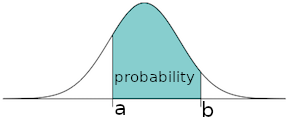
\includegraphics[width=.5\textwidth]{Pictures/normalarea}
\caption{Gráfico de $ y = \frac{1}{\sqrt{2\pi}}e^{-x^2/2} $ e a probabilidade de que $ Z \in [a,b] $ representada pela área esverdeada entre os pontos $ a $ e $ b $.}
\label{fig:normalarea}
\end{figure}

Não demonstraremos o Teorema do Limite Central neste módulo, pois são necessárias ferramentas mais avançadas.

No caso de $ X \sim \Bernoulli(\frac{1}{2}) $, o que corresponde a lançar uma moeda justa, podemos visualizar como a distribuição de $ X_1+\dots+X_n $ se aproxima da função
$ y = \frac{1}{\sqrt{2 \pi}} e^{-x^2/2} $, como ilustrado na Figura~\ref{fig:clt}.

\begin{example}
Ao contar os votos em uma eleição muito disputada, 25.301 votos já foram contados: 12.636 para o Candidato~A e 12.665 para o Candidato~B. Ainda faltam 400 votos para serem contados. Qual é a probabilidade de que o Candidato~B vença a eleição?

Supondo que cada voto seja como uma moeda justa, a pergunta que estamos fazendo é:

\[
\Pb( X_1 + \dots + X_{400} \geq 215 )
\]

onde $ X_1,\dots,X_n $ são independentes e têm distribuição $ \Bernoulli(\frac{1}{2}) $. Pela simetria, isso é o mesmo que:

\[
\Pb( X_1 + \dots + X_{400} \leq 185 )
\]

e, portanto, isso é igual a:

\[
\frac{1}{2} \cdot \Big[ 1 - \Pb( 185 < X_1 + \dots + X_{400} < 215 ) \Big]
\]

Dado que $ \mu = \frac{1}{2} $ e $ \sigma = \frac{1}{2} $, reescrevemos convenientemente o evento como:

\[
\frac{1}{2} - \frac{1}{2} \cdot
\Pb\Big( {-}1.5 < \frac{X_1 + \dots + X_{400}-400\cdot \mu}{\sigma \sqrt{400}} < 1.5 \Big)
\]

e, usando o Teorema do Limite Central, aproximamos por:

\[
\frac{1}{2} - \frac{1}{2} \int_{-1.5}^{1.5} \frac{1}{\sqrt{2 \pi}}
e^{-x^2/2} \, \dd x
\approx
0.07
\]

Você não deve tentar calcular esta integral em casa, a única maneira de obter esse valor é consultando uma tabela, veremos mais sobre isso posteriormente. Portanto, a resposta é 0.07, ou 7%.

Observe que fornecemos apenas uma resposta aproximada com uma figura significativa. Para obter mais precisão do que isso, seriam necessárias considerações mais cuidadosas e seriam o tema de módulos mais avançados.
\end{example}

\begin{figure}[b!]
\centering
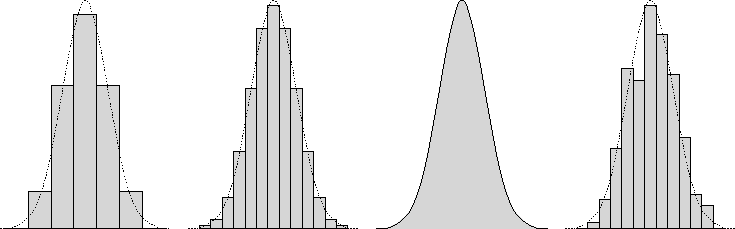
\includegraphics[width=\textwidth]{Pictures/clt}
\caption
{
%The first two graphs are the probability mass functions of $ \Binom(n,\frac{1}{2}) $ rescaled so as to show $ \pm 3 \sigma $.
%The third graph is the graph of $ y = \frac{1}{\sqrt{2\pi}}e^{-x^2/2} $.
%The fourth graph displays the relative frequencies in a random sample of $ 200 $ independent random variables with distribution $ \Binom(16,\frac{1}{2}) $.
Função de probabilidade de $\smash{\frac{S_n - n\mu}{\sigma\sqrt{n}}}$ para $S_n$ com distribuições~$\Binom(4,\frac{1}{2})$ e~$\Binom(16,\frac{1}{2})$ para valores entre $-3$ e $3$.
A área de cada retângulo é dada pela função de probabilidade.
O terceiro gráfico é a função de densidade de uma normal padrão, assim como as linhas pontilhadas.
O quarto gráfico representa as frequências relativas de $\smash{\frac{S_n - n\mu}{\sigma\sqrt{n}}}$ para $S_n$ com distribuição $\Binom(16,\frac{1}{2})$, em um experimento real com~$200$ amostras.
}
\label{fig:clt}
\end{figure}

Também podemos usar as "versões de um lado" do Teorema do Limite Central.
Dessa forma, o exemplo anterior fica simplificado:
\begin{align}
\Pb( X_1 + \dots + X_{400} \geq 215 )
& =
\Pb\Big( \frac{X_1 + \dots + X_{400}-400\cdot \mu}{\sigma \sqrt{400}} \geq 1.5 \Big)
\\ &
\approx
\int_{1.5}^{+\infty}
\tfrac{1}{\sqrt{2 \pi}}
e^{-x^2/2} \, \dd x
\\ &
\approx
0.07.
\end{align}

Se reescrevermos o Teorema do Limite Central como
\[
\Pb\Big( \mu + \frac{\sigma}{\sqrt{n}} a \leq \frac{X_1+\dots+X_n}{n} \leq \mu + \frac{\sigma}{\sqrt{n}} b \Big)
\approx
\int_a^b
\tfrac{1}{\sqrt{2 \pi}}
e^{-x^2/2} \, \dd x
,
\]
obtemos uma boa descrição do comportamento estatístico da média observada $ \frac{X_1+\dots+X_n}{n} $.
Conforme previsto pela lei das médias, a média observada está concentrada em torno de $ \mu $, mas agora podemos dizer algo mais preciso.
A média observada flutua como $ \mu + \sigma \frac{1}{\sqrt{n}} Z $, onde $ Z $ é essa "coisa" descrita por
\[
\Pb(a \leq Z \leq b) =
\int_a^b
\tfrac{1}{\sqrt{2 \pi}}
e^{-x^2/2} \, \dd x
.
\]
Variáveis aleatórias descritas em termos de integrais são chamadas de \emph{variáveis aleatórias contínuas}, que é o tema da próxima seção.


% !TeX spellcheck = pt_BR
% !TEX encoding = UTF-8 Unicode

% Ver copyright.tex para direitos autorais e licença.

\clearpage
\section{Variáveis aleatórias contínuas}

\subsection{Função de densidade de probabilidade}

Considere a variável aleatória $X$ definida informalmente da seguinte maneira: "Seja $X$ um número escolhido no intervalo $(0,1)$ de forma uniforme ao acaso." Ao pensarmos com cuidado, percebemos que essa descrição é um pouco desconcertante. A palavra "uniforme" deveria significar que qualquer número $x \in (0,1)$ tem igual probabilidade de ser escolhido, ou seja, $\Pb(X = x)$ deveria ser o mesmo para cada $x$. No entanto, existem infinitos $x \in (0,1)$, o que forçaria $\Pb(X = x)$ a ser zero. Isso de fato acontecerá para todas as variáveis aleatórias com distribuições contínuas, que definimos agora.

\begin{definition}
Dizemos que uma variável aleatória $X$ é \emph{contínua, com função de densidade de probabilidade $f_X: \R \to \R$}, se
\begin{equation}
\Pb(a \leq X \leq b) = \int_{a}^{b} f_X(x) \, \dd x
\end{equation}
para todo $a < b \in \R$.
\end{definition}

Uma densidade $f_X$ especifica a "probabilidade por unidade de comprimento." É algo análogo à função de probabilidade de massa, mas não exatamente. A probabilidade de $X$ estar em um pequeno intervalo de comprimento $\Delta x$ é dada por $f_X(x) \Delta x$, em vez de $f_X(x)$, e $f_X$ em si pode assumir valores muito grandes em pequenos intervalos. Portanto, é " $f_X(x) \Delta x$ " que é análogo a $p_X(x)$.

Uma função de densidade deve satisfazer necessariamente
\[
\int_{-\infty}^{+\infty} f_X(x) \, \dd x = 1
.
\]

\subsection{Variáveis Uniformes}

Sejam $a$ e $b$ em $\R$ com $a < b$. Uma variável aleatória $X$ tem a distribuição uniforme (contínua) em $(a,b)$ se
\[
f_X(x) =
\begin{cases}
\frac{1}{b-a}&\text{se } a < x < b,\\
0&\text{caso contrário.}
\end{cases}
\]
Escrevemos $X \sim \Unif(a,b)$.\\

Observe que, para qualquer intervalo $[c,d] \subseteq [a,b]$, temos
\[
\Pb(X \in [c,d]) = \int_{c}^d \frac{1}{b-a} \, \dd x
=
\frac{d-c}{b-a}
,
\]
ou seja, o intervalo $[c,d]$ tem uma probabilidade dada pela \emph{proporção} do seu comprimento dentro do intervalo $[a,b]$. Por outro lado, se $c < a$ e $d \in [a,b]$, então
\[
\Pb(X \in [c,d])
=
\frac{d-a}{b-a}
\]
porque a parte do intervalo $[c,d]$ que não se sobrepõe com $[a,b]$ não conta.


\subsection{Distribuição Normal}

Seja $\mu \in \R$ e $\sigma > 0$. Uma variável aleatória $X$ tem distribuição normal (ou gaussiana) com parâmetros $\mu$ e $\sigma^2$ se tiver uma função de densidade de probabilidade dada por
\[
f_X(x) = \frac{1}{\sqrt{2\pi \sigma^2}} \cdot \e ^{-\frac{(x-\mu)^2}{2\sigma^2}}
\]
para todo $ x \in \R $.
Escrevemos $X \sim \Normal (\mu,\sigma^2)$.

O parâmetro $ \mu $ dá o centro da função de densidade, e o parâmetro $ \sigma^2 $ especifica a escala com que essa densidade está sendo alongada.
Através de uma mudança de variáveis na integral, podemos ver que
$X \sim \Normal (\mu,\sigma^2)$
é equivalente a
$ X = \mu + \sigma\cdot Z $ com $ Z \sim \Normal(0,1) $.
De fato, definindo $ Z = \frac{X-\mu}{\sigma} $,
\begin{align}
\Pb(a \leq Z \leq b)
&
=
\Pb(\mu + a\sigma \leq X \leq \mu+ b\sigma)
\\
&
=
\int_{\mu + a\sigma}^{\mu + a\sigma}
\frac{1}{\sqrt{2\pi \sigma^2}} \cdot \e ^{-\frac{(x-\mu)^2}{2\sigma^2}}
\, \dd x
\\
&
=
\int_a^b
\frac{1}{\sqrt{2\pi}} \cdot \e ^{-\frac{z^2}{2}}
\, \dd z
.
\end{align}

\begin{remark}
Não é fácil ver que
$ \int_{-\infty}^{+\infty} f_X(x) \, \dd x = 1 $.
Ao substituir, obtemos
\[
\int_{-\infty}^{+\infty}
\frac{1}{\sqrt{2\pi \sigma^2}} \cdot \e ^{-\frac{(x-\mu)^2}{2\sigma^2}}
\, \dd x
=
\int_{-\infty}^{+\infty}
\frac{1}{\sqrt{\pi}} \cdot \e ^{-u^2}
\, \dd u
.
\]
Portanto, é suficiente verificar que
$ \int_{-\infty}^{+\infty} e^{-x^2} = \sqrt{\pi} $.
Na maioria dos livros didáticos, isso é feito usando coordenadas polares para integrais em $ \R^2 $, mas não queremos usar esse método.
Em vez disso, usamos um truque diferente: trocamos as integrais iteradas em
\[
\int_0^{+\infty}\left(
      \int_0^{+\infty} ye^{-(1+x^2)y^2}\dd y\right)\dd x
=
\int_0^{+\infty}\left(
      \int_0^{+\infty} y e^{-x^2y^2} e^{-y^2} \dd x\right)\dd y
,
\]
o que podemos fazer porque o integrando é não-negativo.
A primeira integral pode ser calculada como
\[
\lim_{z\to{+\infty}}
\int_0^z
ye^{-(1+x^2)y^2}\dd y
=
\lim_{z\to{+\infty}}
\frac{-1}{2(1+x^2)}
\Big[
e^{-(1+x)^2 y^2}
\Big]_0^z
=
\frac{1}{2(1+x^2)}
\]
e
\[
\int_0^{+\infty}\left(
      \int_0^{+\infty} ye^{-(1+x^2)y^2}\dd y\right)\dd x
=
\lim_{z\to{+\infty}}
\int_0^{z}
\frac{1}{2(1+x^2)}
\dd x
=
\lim_{z\to{+\infty}}
\frac{\arctan z}{2}
=
\frac{\pi}{4}
.
\]
A segunda integral pode ser reescrita como
\[
\int_0^{+\infty}
\left( \int_0^{+\infty} e^{-u^2}\dd u \right)
e^{-y^2}\dd y
.
\]
Desta forma, concluímos que
$ \int_{0}^{+\infty} e^{-x^2} = \frac{\sqrt{\pi}}{2} $.
Por simetria,
$ \int_{-\infty}^{+\infty} e^{-x^2} = \sqrt{\pi} $,
que era o que queríamos.
\end{remark}

\subsection{Tempo de Vida Exponencial}

Seja $\lambda > 0$. Uma variável aleatória $X$ tem distribuição exponencial com parâmetro $\lambda$ se
\[
f_X(x) = \begin{cases} \lambda\e ^{-\lambda x} & \text{se } x > 0,
\\
0 & \text{se } x\le 0
.
\end{cases}
\]
Escrevemos $X \sim \Exp(\lambda)$.

Observe que
\[
\Pb(X>t) = e^{-\lambda t}
.
\]

A distribuição exponencial é comumente usada para modelar a vida útil de entidades que têm a propriedade de \textit{falta de memória}, normalmente objetos inanimados que não sofrem efeitos de envelhecimento.
Para explicar o que isso significa, vamos pensar nas lâmpadas. Suponhamos que a vida útil das lâmpadas de uma determinada marca tem uma distribuição Exponencial($\lambda$) (vamos assumir que ligamos a luz e não a desligamos até a lâmpada queimar). Então, a propriedade de falta de memória significa que, independentemente de a lâmpada ter sido ativada recentemente ou ter estado ativa por um certo período de tempo, a distribuição do tempo restante de vida é a mesma. Matematicamente, isso é expresso pela seguinte identidade, que vale para todos~$s,t \ge 0$:
\[\Pb(X>t+s \,|\,  X> t) = \Pb(X > s).\]

\subsection{Esperança}

\begin{definition}
[Esperança]
Seja $ X $ uma variável aleatória contínua com densidade $ f_X $.
Definimos a \emph{esperança} de $ X $, denotada por $ \E[X] $, como o número real dado por
\[
\E[X] = \int_{-\infty}^{+\infty} x \, f_X(x) \, \dd x
,
\]
desde que esta integral convirja absolutamente.
Se a integral convergir absolutamente, dizemos que $ X $ é \emph{integrável}; caso contrário, $ \E[X] $ não está definida.
\end{definition}

\begin{example}
[Uniforme]
Se $X\sim \Unif[a,b]$, então
\[
\E [X] = \int_a^b x \, \frac{1}{b-a} \, \dd x = \frac{a+b}{2}
.
\]
Isso significa que a esperança de uma variável aleatória com distribuição uniforme no intervalo $ [a,b] $ é o ponto médio do intervalo.
\end{example}

\begin{example}
[Exponencial]
Se $X\sim\Exp(\lambda)$,
então, integrando por partes,
\[
\E [X]
=
\int_0^{+\infty} x \lambda e^{-\lambda x} \, \dd x
=
\lim_{u\to{+\infty}}
\Big[
{-x}
e^{-\lambda x}
-
\tfrac{1}{\lambda}
e^{-\lambda x}
\Big]_0^u
=
\frac{1}{\lambda}
.
\qedhere
\]
\end{example}

\begin{example}
[Normal]
Suponha que $X\sim \cN (0,1)$,
Então, substituindo $ u=x^2/2 $,
\[
\int_{0}^{+\infty} x \frac{e^{-x^2/2}}{\sqrt{2\pi}}\dd x
=
\lim_{z\to{+\infty}}
\Big[
\frac{-e^{-x^2/2}}{\sqrt{2\pi}}
\Big]_0^z
=
\frac{1}{\sqrt{{2\pi}}}
.
\]
Por simetria,
\[
\int_{-\infty}^0 x \frac{e^{-x^2/2}}{\sqrt{2\pi}}\dd x
=
-\frac{1}{\sqrt{{2\pi}}}
\]
e, portanto, $ \E[X] = 0 $.
\end{example}

\begin{example}
[Cauchy]
Suponha que $ X $ é uma variável aleatória com densidade
\[
f_X(x)=
\frac{1}{\pi\cdot(1+x^2)}
.
\]
Então
\[
\int_{0}^{+\infty} x f_X(x) \, \dd x
=
\int_{0}^{+\infty} \frac{x}{\pi\cdot(1+x^2)} \dd x
\geq
\int_{1}^{+\infty} \frac{x}{\pi\cdot(1+x^2)} \dd x
,
\]
e assim
\[
\int_{0}^{+\infty} x f_X(x) \, \dd x
\geq
\int_{1}^{+\infty} \frac{1}{2 \pi x} \dd x
=
\frac{1}{2\pi}
\lim_{z\to \infty} \ln z
=
+\infty
.
\]
Neste caso, $ \E[X] $ \emph{não é definida}, apesar da simetria.
Finalmente, temos um exemplo de uma variável aleatória que \emph{não é integrável}!
\end{example}

\subsection{Variância}

\begin{proposition}
Seja $ X $ uma variável aleatória contínua com densidade $ f_X $.
Seja $ g:\R \to \R $ uma função piecewise contínua.
Então
\[
\E[g(X)] = \int_{-\infty}^{+\infty} g(x) \, f_X(x) \, \dd x
\]
se a integral convergir absolutamente, e $ \E[g(X)] $ é indefinida se não convergir absolutamente.
\end{proposition}

A analogia com a função de massa de probabilidade está resumida na Tabela~\ref{table:comparison}.

\begin{example}
[Uniforme]
Se $X\sim \Unif [a,b]$, então
\[
\E [X^2] = \int_a^b \frac{x^2}{b-a} \, \dd x = \frac{a^2+ab+b^2}{3}.
\]
\end{example}

\begin{table}[b!]
\centering
\def\arraystretch{1.7}%
\begin{tabular}{|c|c|}
\hline
$p_X$ 			&	$f_X$	\\
\hline
$p_X:\R\to\R$ 		&	$f_X:\R\to\R$	\\
$p_X(x) \geq 0$ $\forall \, x \in \R$
			& $f_X(x) \geq 0$ $\forall \, x \in \R$ \\
$\Pb(X=x)=p_X(x)$ 	& 	$\Pb(X=x)=0$ \\
$ \Pb(a \leq X \leq b) = \sum_{a \leq x \leq b} p_X(x) $
			& 	$ \Pb(a \leq X \leq b) = \int_a^b f_X(x) \dd x $ \\
$p_X(x)=\Pb(X=x)$ 	& 	definido implicitamente acima \\
$\sum_{x}p_X(x) =1$ & $\int_{-\infty}^{\infty} f_X(x) \, dx=1$ \\
$ p_X(x) \leq 1$ $\forall \, x$ & $f_X(x)$ pode ser $>1$ \\
$ \E[g(X)] = \sum_x g(x) p_X(x) $ & $ \E[g(X)] = \int_{-\infty}^{+\infty} g(x) f_X(x) \dd x $ \\
\hline
\end{tabular}
\caption{Função de massa de probabilidade e função de densidade de probabilidade.}
\label{table:comparison}
\end{table}

\begin{example}
[Exponencial]
Se $X\sim\Exp(\lambda)$,
então, integrando por partes duas vezes,
\[
\E [X^2]
=
\int_0^{+\infty} x^2 \lambda e^{-\lambda x} \, \dd x
=
\lim_{z\to{+\infty}}
\Big[
{-x^2}
e^{-\lambda x}
-
\tfrac{2x}{\lambda}
e^{-\lambda x}
-
\tfrac{2}{\lambda^2}
e^{-\lambda x}
\Big]_0^z
=
\frac{2}{\lambda^2}
.
\qedhere
\]
\end{example}

\begin{example}
[Normal]
Se $X\sim \cN (0,1)$,
então, integrando por partes,
\begin{align}
\E [X^2]
& =
\int_{-\infty}^{+\infty} x^2 \frac{e^{-x^2/2}}{\sqrt{2\pi}}\dd x
\\
&
=
2 \cdot \frac{1}{\sqrt{2\pi}}
\int_{0}^{+\infty} x \cdot (x {e^{-x^2/2}}) \, \dd x
\\
&
=
\frac{2}{\sqrt{2\pi}}
\lim_{u\to+\infty}
\Big[
{-x} {e^{-x^2/2}}
+
\int_{0}^{u}
e^{-x^2/2} \, \dd x
\Big]_0^u
\\
&
=
\frac{2}{\sqrt{2\pi}}
\int_{0}^{+\infty} {e^{-x^2/2}} \, \dd x
=
1
.
\end{align}
\end{example}

\begin{definition}
[Quadrado-integrável]
Como no caso de variáveis aleatórias discretas, dizemos que uma variável aleatória contínua é \emph{quadrado-integrável} se $ X^2 $ for integrável.
\end{definition}

Assim como no caso discreto, se uma variável aleatória for quadrado-integrável, ela será automaticamente integrável (porque $ |x| \leq 1+x^2 $).

\begin{definition}
[Variância]
Seja $ X $ uma variável aleatória contínua quadrado-integrável com densidade $ f_X $ e média $ \mu = \E[X] $.
Definimos a \emph{variância} de $ X $ como
\[
\V (X) = \E\big[ (X - \mu)^2 \big]
.
\]
\end{definition}

Como fizemos no caso de variáveis aleatórias discretas, podemos expandir a definição de variância para obter uma fórmula alternativa:
\[
\V(X) = \E[X^2] - (\E[X])^2
,
\]
que usamos nos exemplos a seguir.

\begin{example}
[Uniforme]
Se $X\sim \Unif [a,b]$, então
\[
\V(X) =
\frac{a^2+ab+b^2}{3}
-
\frac{a^2+2ab+b^2}{4}
= \frac{(b-a)^2}{12} .
\]
\end{example}

\begin{example}
[Exponencial]
Se $X\sim\Exp(\lambda)$,
então
\[ \V(X) = \frac{2}{\lambda^2} - \Big(\frac{1}{\lambda}\Big)^2 = \frac{1}{\lambda^2} .\]
\end{example}

\begin{example}
[Normal]
Se $X\sim\Normal(0,1)$,
então
\[
 \V(X) = 1 - 0^2 = 1 .
\]
\end{example}


\clearpage
\section{Uma única teoria para discretas e contínuas}

\subsection{Função de distribuição cumulativa}

Uma maneira de especificar uma distribuição de probabilidade em $ \R $ é dizer o quanto de probabilidade está à esquerda de cada ponto $ x $.
Em termos de uma variável aleatória $ X $ com a distribuição dada, essa probabilidade é uma função de $ x $.

\begin{definition}
Seja~$X$ uma variável aleatória. A \emph{função de distribuição cumulativa de~$X$} é a função~$F_X: \R \to [0,\infty)$ definida por
\[
F_X(x) = \Pb(X \le x)
\]
para todo $ x \in \R $.
\end{definition}

\subsubsection*{Outras probabilidades a partir de~$F_X$}

Agora, observamos que, embora~$F_X(x)$ seja definido como~$\Pb(X \le x)$, é possível usar~$F_X$ para obter outras probabilidades envolvendo~$X$. Fórmulas importantes são
\[\Pb(X > x) = 1 - \Pb(X \le x) = 1 - F_X(x)\]
e, para~$x < y$,
\[\Pb(x < X \le y) = \Pb(X \le y) - \Pb(X \le x) = F_X(y) - F_X(x).\]

Observe também que
\[\Pb(X = x) > 0 \quad \text{se e somente se}\quad F_X\text{ tem um salto em~$x$}\]
e, nesse caso, o tamanho do salto é a probabilidade de~$X = x$.

\subsubsection*{$F_X$ determina $ \Pb_X $}

\begin{proposition}
Se~$X$ e~$Y$ são duas variáveis aleatórias com~$F_X = F_Y$, então~$X$ e~$Y$ têm a mesma distribuição.
\end{proposition}
Essa proposição nos diz que a função de distribuição cumulativa realmente codifica a distribuição de uma variável aleatória (no sentido de que, dada a função de distribuição cumulativa, há apenas uma distribuição correspondente a ela).

Já vimos que $ F_X $ determina $ \Pb_X(\{x\}) $ para cada $ x \in \R $ e $ \Pb_X((a,b]) $ para todo $ a < b \in \R $.

Faltam-nos as ferramentas necessárias para provar que ela determina $ \Pb_X(B) $ para todo $ B \in \cB $.

\subsection{Casos discretos e contínuos}

\begin{figure}[b!]
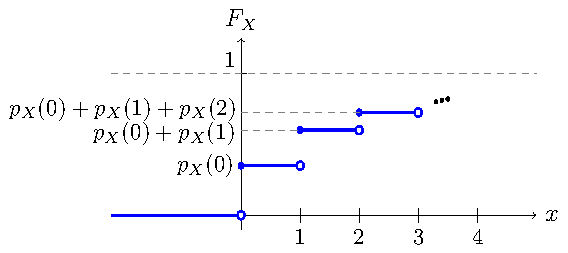
\includegraphics[width=\textwidth]{Pictures/cdfbasic}
\caption{Função de distribuição cumulativa de uma variável aleatória discreta.}
\label{fig:cdfbasic}
\end{figure}

Para obter uma primeira ideia de como se parece uma função de distribuição cumulativa, consideremos o caso em que~$X$ é discreto e tem suporte discreto contido em $\N_0$,
de modo que
\[\sum_{k=0}^\infty \Pb(X =k) = 1.\]
Em seguida, observe primeiro que
$F_X(x) = \Pb(X \le x) = 0$
para todos os $ x < 0  $.
A seguir,
e para todo $x \in [0,1)$,
\[F_X(x) = \Pb(X \le x) = \Pb(X < 0) + \Pb(X = 0) + \Pb(0 < X \le x) = 0 + p_X(0) + 0= p_X(0).\]
Ao argumentar de maneira semelhante, concluímos que
\[F_X(x) = \begin{cases} 0&\text{se } x < 0,\\ p_X(0)&\text{se } x \in [0,1),\\ p_X(0) + p_X(1)&\text{se } x \in [1,2),\\ p_X(0) + p_X(1) + p_X(2)&\text{se } x \in [2,3)\\ \cdots \end{cases}\]

O gráfico de~$F_X$ se parece com o da Figura~\ref{fig:cdfbasic}.

\begin{figure}[t]
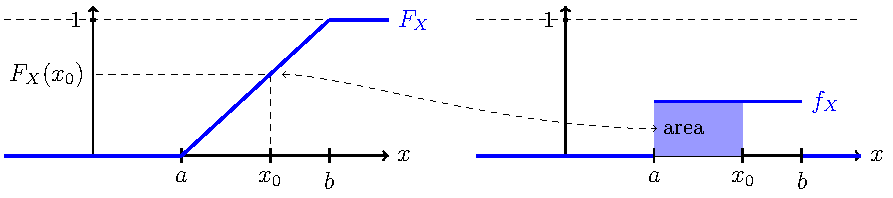
\includegraphics[width=\textwidth]{Pictures/uniform}
\caption{Função de distribuição cumulativa de uma variável aleatória uniforme.}
\label{fig:uniform}
\end{figure}

\begin{figure}[b]
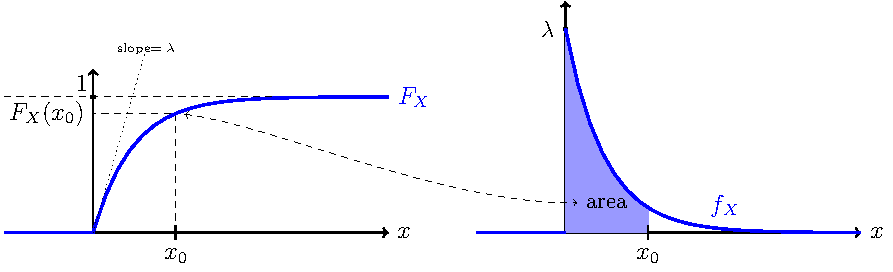
\includegraphics[width=\textwidth]{Pictures/exponential}
\caption{Função de distribuição cumulativa de uma variável aleatória exponencial.}
\label{fig:exponential}
\end{figure}

Se~$X$ for contínuo, então
\[F_X(x) = \Pb(X \le x) = \Pb(X \in (-\infty,x]) = \int_{-\infty}^x f_X(y)\dd y.\]
O teorema fundamental do Cálculo implica então que, nos pontos onde $ f_X $ é contínuo,
\[
f_X(x) = \tfrac{\dd}{\dd x} F_X'(x)
,
\]
ou seja, a função de distribuição cumulativa é diferenciável e sua derivada é a função de densidade de probabilidade.
O gráfico de~$F_X$ se parece com o das Figuras~\ref{fig:uniform} e~\ref{fig:exponential}.


\subsection{Esperança e variância}

É possível fornecer uma definição unificada de esperança de uma variável aleatória, sem assumir que ela seja discreta ou que tenha uma densidade.
Há uma fórmula mágica usando $ F_X $ que funciona simultaneamente para qualquer tipo de variável aleatória.
Não vamos nos preocupar em fornecer tal fórmula, mas é importante ter em mente que a esperança é algo que pode ser definido para qualquer variável aleatória limitada (e, desde que algumas somas ou integrais sejam convergentes, também pode ser definida para variáveis aleatórias ilimitadas).
Novamente, dizemos que $ X $ é \emph{integrável} se $ \E[X] $ for definido e finito.

Essa definição geral de esperança ainda satisfaz as três propriedades:
\begin{itemize}
\item
Unitária: $ \E[\I_A] = \Pb(A) $,
\item
Monótona:
Se $ 0 \leq Z \leq X $ para todo $ \omega\in\Omega $, então $ 0 \leq \E[Z] \leq \E[X] $,
\item
Linear: $ \E[aX+bY]=a\E[X]+b\E[Y] $
\end{itemize}
desde que $ X $ e $ Y $ sejam integráveis.

Não provaremos essas propriedades.
Claro, não poderíamos possivelmente prová-las, pois nem mesmo fornecemos a definição geral de esperança.
Mas mesmo que tivéssemos escrito a fórmula, com as ferramentas atuais não seríamos capazes de provar que a esperança é linear em geral.
A ideia da prova é a seguinte: quaisquer variáveis aleatórias $ X $ e $ Y $ podem ser aproximadas por variáveis aleatórias discretas $ X' $ e $ Y' $ e, uma vez que $ \E[X'+Y']=\E[X']+\E[Y'] $, concluímos que $ \E[X+Y]=\E[X]+\E[Y] $.

Mais uma vez, e $ X $ é \emph{quadraticamente integrável} se $ \E[X^2] $ for finito, e observe que se $ X $ é quadraticamente integrável, então ele é automaticamente integrável (porque $ |x|\leq 1+x^2 $).

\begin{definition}
[Variância]
A \emph{variância} de uma variável aleatória quadraticamente integrável $ X $ é definida como
\[
\V(X) = \E[(X-\E[X])^2]
.
\]
\end{definition}

Observamos que a desigualdade de Chebyshev é válida para qualquer variável aleatória quadraticamente integrável.
De fato, na prova dada na Seção~\ref{sub:chebyshev}, usamos apenas as propriedades de esperança mencionadas acima e nada mais.

\begin{definition}
[Covariância]
Também definimos a \emph{covariância} de duas variáveis aleatórias quadraticamente integráveis como
\[
\Cov(X,Y) = \E[(X-\E[X])(Y-\E[Y])]
\]
e dizemos que elas são \emph{não correlacionadas} se sua covariância for zero.
\end{definition}
Observe que a covariância possui todas as propriedades mencionadas na Seção~\ref{sub:covproperties}.
De fato, a prova dessas propriedades usou apenas as três propriedades de esperança mencionadas acima e nada mais.
Em particular, o Corolário~\ref{cor:uncorrelated} vale em geral, ou seja,
\[
\V(X_1+\dots+X_n)
=
\V(X_1)
+\dots+
\V(X_n)
\]
desde que $ X_1,\dots,X_n $ sejam não correlacionados.

A independência é discutida na próxima seção.



% !TeX spellcheck = pt_BR
% !TEX encoding = UTF-8 Unicode

% Ver copyright.tex para direitos autorais e licença.

\clearpage
\section{Distribuições Conjuntas e Independência}

\subsection{Função de Densidade Conjunta}

Agora explicaremos o que significa para duas variáveis aleatórias seguirem uma distribuição conjunta contínua.

\begin{definition}
[Densidade Conjunta]
Duas variáveis aleatórias~$X$ e~$Y$ definidas no mesmo espaço de probabilidade são chamadas de \emph{conjuntamente contínuas} com uma \emph{função de densidade conjunta} $ f_{X,Y}:\R^2\to\R_+ $
se
\[
\Pb(a_1 \leq X \leq a_2,\; b_1 \leq  Y \leq  b_2)
= \int_{a_1}^{a_2}
\Big(
\int_{b_1}^{b_2} f_{X,Y}(x,y)\;\dd y
\Big)
\dd x
\]
para todo $a_1 < a_2$ e~$b_1 < b_2$.
\end{definition}

As \emph{funções de densidade marginal} são dadas por:
\[f_X(x) = \int_{-\infty}^\infty f_{X,Y}(x,y) \dd y\qquad \text{e}\qquad f_Y(y) = \int_{-\infty}^\infty f_{X,Y}(x,y) \dd x.\]
Em resumo, densidades marginais são obtidas da densidade conjunta "integrando" a outra variável.

\begin{example}
Considere o quadrado $ Q = \{(x,y) \in \R^2:|x|+|y|<1\} $, e suponha que a função de densidade conjunta de $ X $ e $ Y $ seja $ f_{X,Y}(x,y) = \frac{1}{2} \I_Q(x,y) $.
Podemos determinar a função de densidade marginal de $ X $ integrando:
\[
f_X(x) = \int_{-\infty}^{+\infty} \tfrac{1}{2} \I_Q(x,y) \, \dd y = (1-|x|) \I_{[-1,1]}(x).
\]
Se integrarmos em relação a $ x $, obtemos $ f_Y(y) = (1-|y|) \I_{[-1,1]}(y) $.
\end{example}

\subsection{Função de Distribuição Conjunta}

\begin{definition}
Sejam~$X,Y$ variáveis aleatórias.
A \emph{função de distribuição conjunta de~$(X,Y)$} é a função~$F_{X,Y}:\R^2 \to [0,1]$ dada por
\[
F_{X,Y}(x,y) = \Pb(X \le x,\; Y \le y)
\]
para todo $ x, y \in \R $.
\end{definition}

Para variáveis discretas, essa definição se reduz a
\[
F_{X,Y}(x,y) =
\sum_{s \leq x} \sum_{t \leq y} p_{X,Y}(s,t)
\]
para todo $ x,y\in\R $.
Para variáveis aleatórias conjuntamente contínuas, a função de distribuição conjunta
é dada por
\[
F_{X,Y}(x,y) = \int_{-\infty}^x \int_{-\infty}^y f_{X,Y}(s,t)\;\dd t\;\dd s
.
\]
De qualquer forma, é possível recuperar a função de massa de probabilidade conjunta e a função de densidade de probabilidade conjunta a partir da função de distribuição conjunta, mas não entraremos em detalhes sobre isso.

\subsection{Independência}

\begin{definition}
[Independência de Duas Variáveis Aleatórias]
Dadas duas variáveis aleatórias $ X $ e $ Y $, dizemos que \emph{$ X $ e $ Y $ são independentes} se
\[
\Pb(X \in A, Y\in B)
=
\Pb(X \in A)
\Pb(Y\in B)
\]
para todos os conjuntos $ A, B \in \cB $.
\end{definition}
Para variáveis aleatórias discretas, essa definição é equivalente a
\[
p_{X,Y}(x,y) = p_X(x) \cdot p_Y(y)
\]
para todos os valores $ x,y\in\R $, conforme explicado na Seção~\ref{sub:independencerv}.

Surpreendentemente, a função de distribuição conjunta é capaz de capturar se duas variáveis aleatórias são independentes ou não.

\begin{proposition}
Duas variáveis aleatórias $ X $ e $ Y $ são independentes se e somente se
\[
F_{X,Y}(x,y)
=
F_{X}(x)
F_{Y}(y)
\]
para todo $ x,y\in\R $.
\end{proposition}
\begin{proof}
[Fragmento da prova]
Para $ A = (a,b] $ e $ B= (c,d] $, expandimos para obter
\begin{align}
\MoveEqLeft
\Pb(a<X\leq b, c<Y\leq d)
=
\Pb(a<X\leq b, Y \leq d)
-
\Pb(a<X\leq b, Y \leq c)
\\
&=
\Pb(X\leq b, Y \leq d)
-
\Pb(X \leq a, Y \leq d)
-
\Pb(a<X\leq b, Y \leq c)
\\
&=
F_{X,Y}(b,d)
-
F_{X,Y}(a,d)
-
[ F_{X,Y}(b,c) - F_{X,Y}(a,c) ]
\\
&=
F_{X}(b)
F_{Y}(d)
-
F_{X}(a)
F_{Y}(d)
-
[
F_{X}(b)
F_{Y}(c)
-
F_{X}(a)
F_{Y}(c)
]
\\
&=
[
F_{X}(b)
-
F_{X}(a)
]
\cdot
[
F_{Y}(d)
-
F_{Y}(c)
]
\\
&=
\Pb(a<X\leq b)
\Pb(c<Y\leq d)
.
\end{align}
Portanto,
$ \Pb(X \in A, Y\in B)
=
\Pb(X \in A)
\Pb(Y\in B) $
quando tanto $ A $ quanto $ B $ são compostos por uma união de intervalos finitos desse tipo (abertos à esquerda e fechados à direita).
O caso de conjuntos mais gerais $ A $ e $ B $ requer ferramentas que atualmente não possuímos.
\end{proof}

Para variáveis aleatórias conjuntamente contínuas, a situação é um pouco mais complicada.
Suponha que $ X $ e $ Y $ tenham $ f_X $ e $ f_Y $ como funções de densidade.
Então, elas são independentes se e somente se forem conjuntamente contínuas com uma função de densidade conjunta dada por
\[
f_{X,Y}(x,y)
=
f_{X}(x)
f_{Y}(y)
\]
para todo $ x,y\in\R $.
No entanto, se nos for fornecida uma função de densidade conjunta $ f_{X,Y} $ e desejarmos mostrar que $ X $ e $ Y $ \emph{não} são independentes, não basta encontrar um único ponto $ (x,y) $ tal que
$ f_{X,Y}(x,y) \ne f_{X}(x)f_{Y}(y) $.
Precisamos verificar que $ f_{X,Y}(x,y) \ne f_{X}(x)f_{Y}(y) $ para todos os $ x \in [a,b] $ e todos os $ y \in [c,d] $ para alguns intervalos não degenerados $ [a,b] $ e $ [c,d] $.
Isso ocorre porque, ao contrário da função de massa de probabilidade, as funções de densidade de probabilidade não são únicas, e podemos modificá-las em um único ponto, fazendo com que a identidade mostrada acima deixe de ser válida.

\begin{theorem}
Se $ X $ e $ Y $ são variáveis aleatórias independentes integráveis, então $ XY $ é integrável e
\[
\E[XY] = \E[X] \cdot \E[Y].
\]
Em particular, variáveis aleatórias independentes quadrado-integráveis são não correlacionadas.
\end{theorem}

Nós fornecemos uma prova assumindo que $ X $ e $ Y $ são discretas.
Uma prova que funcione no caso geral requer ferramentas que atualmente não temos.
Quanto à linearidade da esperança, ela se baseia no fato de que qualquer variável aleatória pode ser aproximada por variáveis aleatórias discretas, reduzindo o problema ao caso que já conhecemos.

\begin{definition}
[Independência par a par]
Dizemos que uma coleção de variáveis aleatórias $ X_1, X_2, X_3, \dots $ é \emph{independente par a par} se $ X_j $ e $ X_k $ forem independentes para todo $ j \neq k $.
\end{definition}

\begin{definition}
[Independência mútua]
Dizemos que uma coleção de variáveis aleatórias discretas $ X_1, X_2, X_3, \dots $ é \emph{mutuamente independentes} se, para todo $ k $ e todo $ A_1, \dots, A_k \in \cB $, tivermos
\[
\Pb(X_1\in A_1,\dots,X_k\in A_k)
=
\Pb(X_1\in A_1)
\cdots
\Pb(X_k\in A_k)
.
\]
\end{definition}

Existem condições análogas para independência mútua quando as variáveis aleatórias são contínuas ou discretas, e também uma condição equivalente em termos de funções de distribuição cumulativa conjunta.
Mas não entraremos em detalhes sobre isso.

\subsection{Covariância e a lei das médias}

Como mencionado na seção anterior, se $ X_1,\dots,X_n $ são variáveis aleatórias não correlacionadas, então
\[
\V(X_1+\dots+X_n)
=
\V(X_1)
+\dots+
\V(X_n)
.
\]

Usando isso e a desigualdade de Chebyshev, podemos novamente provar a lei das médias para qualquer sequência de variáveis aleatórias não correlacionadas com a mesma média $ \mu $ e a mesma variância $ \sigma^2 $, sem assumir que sejam discretas.
A prova é idêntica à vista na Seção~\ref{sub:prooflln}.

O Teorema do Limite Central também se aplica a qualquer sequência de variáveis aleatórias quadrado-integráveis mutuamente independentes com a mesma distribuição, sem assumir que sejam discretas.

\clearpage
\section{Somas de variáveis aleatórias independentes}

Somas de variáveis aleatórias independentes surgem em muitos contextos diferentes.
Dadas duas variáveis aleatórias independentes $ X $ e $ Y $, qual é a distribuição de $ X+Y $?

Se $ X $ e $ Y $ são ambas discretas, $ X+Y $ é discreta e sua função de massa de probabilidade pode ser calculada usando a Lei da Probabilidade Total:
\begin{align}
p_{X+Y}(z)&=\sum_{x}\Pb(X=x,Y=z-x)=\sum_{x}\Pb(X=x)\Pb(Y=z-x) \\
&= \sum_{x}p_{X}(x)p_{Y}(z-x).
\end{align}

\begin{example}
\label{exem:somaBernoulli}
Suponha que $X\sim \Binom(n,p)$ e $Y\sim \Binom(m,p)$.
A função de massa de probabilidade de $ X+Y $ pode ser obtida da seguinte forma:
\begin{align}
p_{X+Y}(k)&=\sum_{j=0}^\infty\Pb(X=j)\Pb(Y=k-j) \\
&= \sum_{j=0}^k \tbinom{n}{j}p^j(1-p)^{n-j}\tbinom{m}{k-j}p^{k-j}(1-p)^{m-k+j} \\
&= p^{k}(1-p)^{m+n-k}\sum_{j=0}^k \tbinom{n}{j}\tbinom{m}{k-j} \\
&= \tbinom{n+m}{k}p^{k}(1-p)^{m+n-k}.
\end{align}
\end{example}

Quando as variáveis $ X $ e $ Y $ são independentes e têm densidades $ f_X $ e $ f_Y $, temos a relação análoga a seguir
\[
f_{X+Y}(z)= \int_{-\infty}^{+\infty} f_{X}(x)f_{Y}(z-x)\, \dd x
.
\]

\begin{example}
[Exponenciais e Gama]
Sejam~$X$ e~$Y$ independentes, ambas com a distribuição Exponencial com parâmetro~$\lambda >0$, ou seja,
\[f_X(x) = f_Y(x) =\begin{cases} \lambda \e ^{-\lambda x}&\text{se } x > 0;\\ 0&\text{caso contrário.} \end{cases}\]
Seja~$Z := X+Y$.
Queremos calcular
\begin{align*}
 f_Z(z) &= \int_{-\infty}^\infty f_X(x)\cdot f_Y(z-x)\;\dd x.
 \end{align*}
Agora, observe que o produto dentro da integral é igual a zero quando~$x < 0$ (pois~$f_X(x) = 0$ nesse caso) e quando~$x > z$ (pois~$f_Y(z-x)= 0$ nesse caso). A integral é então igual a
\begin{align*}\int_0^z \lambda \e ^{-\lambda x}\cdot \lambda \e ^{-\lambda(z-x)}\;\dd x &= \lambda^2\cdot \int_0^z\e ^{-\lambda z} \;\dd x = \lambda^2\cdot z\cdot \e ^{-\lambda z}.\end{align*}
A distribuição acima corresponde a uma distribuição Gama com parâmetros $ 2 $ e $ \lambda $.
Em geral, $ Z $ tem distribuição Gama com parâmetros $ n $ e $ \lambda $ se a sua densidade for dada por $ f_Z(z) = \frac{\lambda^n}{(n-1)!}\cdot z^{n-1} \cdot \e ^{-\lambda x} $ para $ z \geq 0 $.
\end{example}

O caso em que $ X $ e $ Y $ são normais é tão importante que o apresentamos como uma proposição.

\begin{proposition}
Se $X_1\sim \No (\mu_1,\sigma_1^2)$ e $X_2\sim \No (\mu_2,\sigma_2^2)$ são independentes.
Então $X_1 +X_2\sim \No (\mu_1 +\mu_2,\sigma_1^2 +\sigma_2^2)$.
\end{proposition}
\begin{proof}
Como $X_1 - \mu_1 \sim \No (0,\sigma_1^2) $ e $X_2 - \mu_2 \sim \No (0,\sigma_2^2) $, podemos supor que $\mu_1=\mu_2=0$.
Após manipulações algébricas longas e trabalhosas, é possível obter
\begin{align}
f_{X+Y}(z)= \frac{1}{2\pi\sigma_1\sigma_2}
\int_{-\infty}^{+\infty}
e^{-\frac{(z-x)^2}{2 \sigma_2^2}}
e^{-\frac{x^2}{2 \sigma_1^2}}
\, \dd x
=
\cdots
=
\tfrac{1}{\sqrt{2\pi(\sigma_1^2+\sigma_2^2)}}
\cdot
e^{-\frac{z^2}{2(\sigma_1^2 + \sigma_2^2) }}
.
\end{align}
Portanto, $f_{X+Y}$ é a densidade correspondente à distribuição $\No (0,\sigma_1^2 + \sigma_2^2)$, que era o que queríamos mostrar.
\end{proof}


\clearpage
\section{Momentos e funções geradoras de momentos}

\begin{definition}
Dada uma variável aleatória $ X $, definimos a \emph{função geradora de momentos de $ X $} como a função $ M_X $ dada por
\[
M_X(t) = \E[e^{tX}]
\]
para os valores de $ t $ para os quais $ e^{tX} $ é integrável.
\end{definition}

\begin{example}
[Geométrica]
Se $X\sim \Geom(p)$, então
\begin{align*}
M_{X}(t)
&=
\sum_{n=1}^{\infty} e^{tn} p (1-p)^{n-1}
=
\begin{cases}
\frac{p}{e^{-t} + p-1}, & t < \ln \tfrac{1}{1-p},
\\
+\infty, & t \geq \ln \tfrac{1}{1-p}.
\end{cases}
\qedhere
\end{align*}
\end{example}

\begin{example}
[Poisson]
\label{exem:fgPoisson}
Se $X\sim \Poisson(\lambda )$, então
\begin{align*}
M_{X}(t) &
=
\sum_{n=0}^{\infty} e^{tn} \frac{e^{-\lambda} \lambda^n}{n!}
=
e^{-\lambda} \sum_{n=0}^{\infty} \frac{(\lambda e^t)^n}{n!}
=
e^{-\lambda} e^{\lambda e^t}
=
e^{\lambda (e^{t}-1)}
.
\qedhere
\end{align*}
\end{example}

\begin{example}
[Normal]
Seja~$X$ uma variável aleatória normal com parâmetros~$\mu$ e~$\sigma^2$, ou seja,
\[f_X(x) = \frac{1}{\sqrt{2\pi \sigma^2}} \cdot \e ^{-\frac{(x-\mu)^2}{2\sigma^2}},\quad x \in \R.\]
A função geradora de momentos de~$X$ pode ser calculada da seguinte forma:
\begin{align}
 \nonumber M_X(t)&= \int_{-\infty}^\infty \e ^{tx}\cdot f_X(x)\;\dd x\\[.2cm]
\nonumber &= \int_{-\infty}^\infty \e ^{tx}\cdot \frac{1}{\sqrt{2\pi\sigma^2}} \cdot \e ^{-\frac{(x-\mu)^2}{2\sigma^2}}\;\dd x\\[.2cm]
 &= \int_{-\infty}^\infty \frac{1}{\sqrt{2\pi\sigma^2}} \cdot \exp\left\{-\frac{1}{2\sigma^2}[(x-\mu)^2 - 2\sigma^2 t x]\right\}\;\dd x \label{eq_gauss}
 \end{align}

Agora, completamos o quadrado:
\begin{align*}
 (x-\mu)^2 - 2\sigma^2 t x &= x^2 - 2(\mu +\sigma^2 t)\cdot x + \mu^2 \\[.2cm]
 &= x^2 - 2(\mu +\sigma^2 t)\cdot x +\mu^2 \;\pm (2\mu \sigma^2 t+ \sigma^4t^2 )\\[.2cm]
 &= (x-\mu-\sigma^2 t)^2 - 2\mu \sigma^2 t- \sigma^4t^2 .
\end{align*}
Isso dá
\[-\frac{1}{2\sigma^2}[(x-\mu)^2 - 2\sigma^2 t x] = -\frac{(x-\mu-\sigma^2 t)^2}{2\sigma^2} +t\mu+ \frac{\sigma^2t^2}{2}.\]
A integral em~\eqref{eq_gauss} então se torna
\[\exp\left\{t\mu + \frac{\sigma^2t^2}{2}\right\}\cdot \int_{-\infty}^\infty \frac{1}{\sqrt{2\pi\sigma^2}} \cdot \exp\left\{-\frac{(x-\mu-\sigma^2t^2)^2}{2\sigma^2}\}\right\} \;\dd x.\]
Agora, observe que a função sendo integrada é a função de densidade de probabilidade de~$\Normal (\mu+\sigma^2 t,\;\sigma^2)$, então a integral é igual a~$1$. Em conclusão,
\[M_X(t) = \exp\left\{t\mu + \frac{\sigma^2 t^2}{2}\right\},\quad t \in \R.\]
\end{example}

\begin{definition}
[Momentos]
Definimos o $ k $-ésimo momento de uma variável aleatória $ X $ como $ \E[X^k] $ se $ X^k $ for integrável.
\end{definition}

O nome "função geradora de momentos" vem do seguinte fato.
\begin{proposition}
Se $ M_X(t) $ é definido em $ (-a,a) $ para algum $ a>0 $, então $ X $ tem todos os momentos e eles são dados por
\[
\E[X^k]
=
M_X^{(k)}(0)
,
\]
onde $ M_X^{(k)} $ denota a $ k $-ésima derivada da função $ M_X $.
\end{proposition}

Não temos as ferramentas para provar esta proposição, mas se estivermos dispostos a ser atrevidos, podemos fazer:
\[
\left. \tfrac{\dd^{k}}{\dd t^{k}}M_{X}(t)\right.
=
\left. \tfrac{\dd^{k}}{\dd t^{k}} \, \E [e^{tX}] \right.
=
\E \left[ \left. \tfrac{\dd^{k}}{\dd t^{k}} \, e^{tX} \right.
\right]
=
\E [X^{k}e^{tX}]
\]
e, avaliando em $ t=0 $, obtemos a proposição.

\begin{example}
[Geométrica]
Se $X\sim \Geom(p)$, então
\begin{equation*}
\E [X] = M_X'(0) = \tfrac{1}{p}
,
\
\E [X^2] = M_X''(0) = \tfrac{2}{p^2} - \tfrac{1}{p}
,
\
\V [X] = \E [X^2] - (\E [X])^2 = \tfrac{1-p}{p^{2}}
.
\qedhere
\end{equation*}
\end{example}

\begin{example}
[Poisson]
Se $X\sim \Poisson(\lambda )$, então
\begin{equation*}
\E [X] = M_X'(0) = \lambda
,
\
\E [X^2] = M_X''(0) = \lambda^2 + \lambda
,
\
\V [X] = \E [X^2] - (\E [X])^2 = \lambda
.
\qedhere
\end{equation*}
\end{example}

\begin{example}
[Normal]
Seja~$X \sim \Normal (\mu,\sigma^2)$. Vamos calcular sua média (ou seja, sua esperança) e variância.
No exemplo anterior, provamos que~$M_X(t)$ está definido para todos~$t \in \R$, com
\[M_X(t) = \exp\left\{\frac{t^2\sigma^2}{2} + \mu t\right\}.\]
Em seguida, usamos o teorema acima para calcular
\begin{align*}
 \E[X] &=\left. \frac{\dd }{\dd t}M_X(t)\right\vert_{t=0} = \left[ (t\sigma^2 + \mu)\cdot \exp\left\{\frac{t^2 \sigma^2}{2}+\mu t\right\}\right]_{t=0} = \mu
 \end{align*}
e
\begin{align*}
 \E[X^2] &=\left. \frac{\dd ^2}{\dd ^2t}M_X(t)\right\vert_{t=0}
= \cdots
=
\sigma^2 + \mu^2.
 \end{align*}
Portanto,
\[\V (X) = \E[X^2] - (\E[X])^2 = \sigma^2 + \mu^2 - \mu^2 = \sigma^2.\]
Esta é a razão pela qual~$X$ é dito ser uma variável aleatória normal com média~$\mu$ e variância~$\sigma^2$.
\end{example}

\begin{proposition}
Para todos $a, b \in \R$,
\[
M_{aX+b}(t) = \e ^{tb}\cdot M_X(at)
\]
para todo $ t $ no qual as funções geradoras de momentos estão definidas.
\end{proposition}

\begin{proof}
Nós calculamos
\[
M_{aX+b}(t) = \E[\e ^{t(aX+b)}] = \e ^{tb}\cdot \E[\e ^{t(aX)}] = \e ^{tb}\cdot M_X(at).
\qedhere
\]
\end{proof}

\begin{proposition}
Quando $ X $ e $ Y $ são independentes,
\[
M_{X+Y}(t) = M_X(t) \cdot M_Y(t)
\]
para todo $ t $ no qual as funções geradoras de momentos estão definidas.
\end{proposition}

\begin{proof}
Se~$X$ e~$Y$ são independentes, então~$\e ^{tX}$ e~$\e ^{tY}$ também são. Portanto,
\[M_{X+Y}(t) = \E[\e ^{t(X+Y)}] = \E[\e ^{tX}\cdot \e ^{tY}] = \E[\e ^{tX}] \cdot \E[\e ^{tY}] = M_X(t)\cdot M_Y(t)
.
\qedhere
\]
\end{proof}

\begin{example}
[Soma de variáveis de Poisson independentes]
Sejam $X\sim\Poisson(\lambda)$ e $Y\sim\Poisson(\mu)$ independentes.
Então
\[
M_{X+Y}(t) = M_{X}(t) \cdot M_Y(t) = e^{\lambda(e^{t}-1)}e^{\mu(e^{t}-1)} = e^{(\lambda+\mu)(e^{t}-1)} = M_Z(t),
\]
onde $Z \sim \Poisson(\lambda+\mu)$.
Isso implica que $X+Y \sim \Poisson(\lambda+\mu)$?
\end{example}

O exemplo acima nos faz pensar se conhecer a função geradora de momentos de uma variável aleatória nos diz qual é a distribuição da variável aleatória. E, de fato, este é o caso.

\begin{theorem}
[A função geradora de momentos determina a distribuição]
Dadas duas variáveis aleatórias $X$ e $Y$, se existe $a>0$ tal que
$M_X(t)$ e $M_Y(t)$ são finitas e coincidem para todo $t \in [-a,a]$, então $X$ e $Y$ têm a mesma distribuição.
\end{theorem}

Também omitimos a prova deste teorema, observando que ela requer ferramentas ainda mais difíceis de construir do que outras provas omitidas nestas notas.

\begin{example}
[Soma de variáveis de Poisson independentes]
Se $X\sim\Poisson(\lambda)$ e $Y\sim\Poisson(\mu)$ são independentes, então $X+Y \sim \Poisson(\lambda+\mu)$.
\end{example}

\begin{example}
[Soma de variáveis normais independentes]
Sejam~$X$ e~$Y$ duas variáveis normais independentes, com médias~$\mu_X$ e~$\mu_Y$ e variâncias~$\sigma^2_X$ e~$\sigma^2_Y$, respectivamente. Também sejam~$a$ e~$b \in \R$ com~$a \ne 0$. Vamos determinar as distribuições de~$aX+b$ e de~$X+Y$. Na última aula, mostramos que
\[M_X(t) = \exp\left\{\frac{t^2\sigma_X^2}{2} + t \mu_X \right\},\qquad M_Y(t) = \exp\left\{\frac{t^2\sigma_Y^2}{2} + t \mu_Y \right\}.\]
Temos que
\[M_{aX+b}(t) = \e ^{tb}\cdot M_X(at) = \e ^{tb}\cdot \exp\left\{ a\mu_X t + \frac{a^2\sigma_X^2t^2}{2}\right\} = \exp\left\{ (a\mu_X + b)t + \frac{a^2 \sigma_X^2 t^2}{2}\right\}. \]
Portanto,~$aX+b$ tem a mesma função geradora de momentos que uma variável aleatória~$\Normal (a\mu+b,a^2\sigma^2)$.
Já que esta função geradora de momentos é definida em uma vizinhança da origem (na verdade, em toda a reta real), concluímos que~$aX+b \sim \Normal (a\mu_X+b,a^2\sigma_X^2)$.

Em seguida, como~$X$ e~$Y$ são independentes, temos
\begin{align*}M_{X+Y}(t) = M_X(t)\cdot M_Y(t) &= \exp\left\{\mu_X t + \frac{\sigma_X^2 t^2}{2}\right\} \cdot \exp\left\{\mu_Y t + \frac{\sigma_Y^2 t^2}{2}\right\} \\[.2cm]
&= \exp\left\{(\mu_X+ \mu_Y) t + \frac{(\sigma_X^2+ \sigma^2_Y) t^2}{2}\right\}.\end{align*}
Isso mostra que~$X+Y$ tem a mesma função geradora de momentos que uma variável aleatória~$\Normal (\mu_X + \mu_Y, \sigma_X^2 + \sigma_Y^2)$.
Já que esta função geradora de momentos é definida em um intervalo aberto que contém zero, concluímos que~$X+Y \sim \Normal (\mu_X + \mu_Y, \sigma_X^2 + \sigma_Y^2)$.
\end{example}



% !TeX spellcheck = pt_BR
% !TEX encoding = UTF-8 Unicode

% Ver copyright.tex para direitos autorais e licença.

\clearpage

\appendix


\section{Somas úteis}

\begin{align*}
&
(a+b)^n = \sum_{j=0}^{n} \binom{n}{j} a^j b^{n-j}
 &&
a,b \in \R, n \in \N_0
\\
&
\sum_{n=0}^\infty x^n = \frac{1}{1-x}
 &&
0 < x < 1
\\
&
\sum_{n=0}^\infty n x^{n-1} = \frac{1}{(1-x)^2}
 &&
0 < x < 1
\\
&
\sum_{n=0}^\infty n (n-1) x^{n-2} = \frac{2}{(1-x)^3}
 &&
0 < x < 1
\\
&
\sum_{n=0}^\infty n (n-1) (n-2) x^{n-3} = \frac{3!}{(1-x)^4}
 &&
0 < x < 1
\\
&
\sum_{k=0}^\infty \frac{x^k}{k!} = e^x
 &&
x \in \R
\\
&
\sum_{k=1}^n k = \frac{n(n+1)}{2}
 &&
n \in \N
\\
&
\sum_{k=1}^n k^2 = \frac{n(n+1)(2n+1)}{6}
 &&
n \in \N
\end{align*}

As cinco primeiras são:
teorema binomial,
série geométrica,
derivada da série geométrica,
segunda derivada da série geométrica,
terceira derivada da série geométrica.
Acontece que é legítimo diferenciar uma série da forma $ \sum_n a_n x^n $ termo a termo, mas não estamos preocupados com os detalhes de por que isso é verdade.

A quinta é a chamada "série de Taylor" da função exponencial.
Para verificar se a fórmula faz sentido, observe que ambos os lados resultam em $ 1 $ para $ x=0 $ e cada lado é igual à sua própria derivada.
Esses dois fatos implicam que ambos os lados são iguais para todos os valores de $ x $, mas não estamos preocupados com os detalhes disso.

As duas últimas fórmulas, uma vez escritas, podem ser provadas por indução (suponha que sejam corretas para um certo valor de $ n $, mostre que são corretas para $ n+1 $).
Se você está curioso sobre como essas fórmulas surgiram, elas podem ser derivadas fazendo inicialmente um palpite educado de que devem ser representadas por polinômios um grau maior do que o termo somado e, em seguida, usando os dois ou três primeiros termos para escrever um sistema de equações para os coeficientes.

\clearpage
\section{Exponenciais superam polinômios}

Para todo $ x \geq 0 $ e $ n \in \N $,
\[
e^x
\geq
1 + x + \frac{x^2}{2} + \frac{x^3}{3!} + \dots + \frac{x^n}{n!}
\]
\begin{proof}
Para $ n=0 $, já sabemos que $ e^x \geq 1 $.
Para $ n=1 $,
\[
e^x
=
1 + \int_0^x e^x \, \dd x
\geq
1 + \int_0^x 1 \, \dd x
=
1+x
\]
Para $ n=2 $,
\[
e^x
=
1 + \int_0^x e^x \, \dd x
\geq
1 + \int_0^x (1+x) \dd x
=
1+x+\tfrac{x^2}{2}
\]
Para $ n=3 $,
\[
e^x
=
1 + \int_0^x e^x \, \dd x
\geq
1 + \int_0^x (1+x+\tfrac{x^2}{2}) \dd x
=
1+x+\tfrac{x^2}{2}+\tfrac{x^3}{3!}
.
\]
O padrão é claro.
\end{proof}

Isso implica que
\[
\frac{a_0 + a_1 x + \dots + a_n x^n}{e^{ax}}
\]
tende a $ 0 $ à medida que $ x \to +\infty $, para todo $ a>0 $.

\begin{proof}
De fato, como $ e^{ax} \geq \frac{a^{n+1}}{(n+1)!} x^{n+1} $, cada termo em
\[
\frac{a_0}{e^{ax}}
+
\frac{a_1 x}{e^{ax}}
+ \dots +
\frac{a_n x^n}{e^{ax}}
\]
está se aproximando de zero à medida que $ x $ aumenta.
\end{proof}

Isso é útil ao calcular integrais impróprias que incluem polinômios e funções exponenciais.



\end{document}



